\documentclass[11pt]{article}
% Preamble for the paper on \SAI (generic part adapted from ../../solomonoff-operator-induction/paper/preamble.tex).
% Section files must not redefine these macros; new global macros are added only by the planning editor (NOTATION.md).
\usepackage[utf8]{inputenc}
\usepackage[T1]{fontenc}
\usepackage{lmodern}
\usepackage[margin=1.05in]{geometry}
\usepackage{amsmath,amssymb,amsthm,mathtools}
\usepackage{stmaryrd}
\usepackage{booktabs,tabularx,array,longtable,multirow}
\usepackage{enumitem}
\usepackage{graphicx}
\usepackage{xcolor}
\usepackage{xspace}
\usepackage{tikz}
\usepackage{url}
\usepackage[hidelinks]{hyperref}
\usepackage[capitalise,noabbrev]{cleveref}
\setlist{itemsep=2pt,topsep=4pt}
\setlength{\emergencystretch}{2em}% lets TeX loosen a line instead of overflowing

% ---- theorem environments (one counter, numbered within section)
\theoremstyle{plain}
\newtheorem{theorem}{Theorem}[section]
\newtheorem{proposition}[theorem]{Proposition}
\newtheorem{lemma}[theorem]{Lemma}
\newtheorem{corollary}[theorem]{Corollary}
\newtheorem{conjecture}[theorem]{Conjecture}
\theoremstyle{definition}
\newtheorem{definition}[theorem]{Definition}
\newtheorem{example}[theorem]{Example}
\newtheorem{assumption}[theorem]{Assumption}
\newtheorem{question}[theorem]{Question}
\theoremstyle{remark}
\newtheorem{remark}[theorem]{Remark}
\crefname{theorem}{Theorem}{Theorems}
\crefname{proposition}{Proposition}{Propositions}
\crefname{lemma}{Lemma}{Lemmas}
\crefname{corollary}{Corollary}{Corollaries}
\crefname{conjecture}{Conjecture}{Conjectures}
\crefname{definition}{Definition}{Definitions}
\crefname{example}{Example}{Examples}
\crefname{assumption}{Assumption}{Assumptions}
\crefname{question}{Question}{Questions}
\crefname{remark}{Remark}{Remarks}
\crefname{appendix}{Appendix}{Appendices}
\crefname{table}{Table}{Tables}
\crefname{figure}{Figure}{Figures}

% ---- status and provenance markers (binding: on every result; they PRINT NOTHING)
% \status{proved} | \status{proved, given X} | \status{computed} | \status{known} | \status{proof sketch}
% | \status{conjecture} | \status{open} | \status{refuted} | \status{assessment}; parts: \status{(a) proved; (b) proof sketch}
% \src{<thread> <item>}: the item in research/tracks/<thread>/notes-final.md (e.g. \src{fundamentals Thm 5.1}).
% Their content is rendered in prose ("we prove", "a computation shows (code in the accompanying repository)").
% Both macros swallow the space that follows them, so an inline call leaves no double space.
\newif\ifsaishowstatus
\saishowstatusfalse % internal checking only: \saishowstatustrue prints them as small grey notes
\newcommand{\status}[1]{\ifsaishowstatus\textup{\textsf{\small[#1]}}\fi\ignorespaces}
\newcommand{\src}[1]{\ifsaishowstatus\unskip\hskip0pt plus 1fil\penalty300\hskip0.35em plus -1fil\relax\textup{\textcolor{gray}{\scriptsize\textsf{#1}}}\fi\ignorespaces}
% abbreviated cross-reference names, for use inside table floats only
\newcommand{\crefabbrev}{\crefname{proposition}{Prop.}{Props.}\crefname{theorem}{Thm.}{Thms.}%
  \crefname{lemma}{Lem.}{Lems.}\crefname{corollary}{Cor.}{Cors.}\crefname{remark}{Rem.}{Rems.}%
  \crefname{example}{Ex.}{Exs.}\crefname{definition}{Def.}{Defs.}\crefname{conjecture}{Conj.}{Conjs.}\crefname{question}{Q.}{Qs.}%
  \crefname{assumption}{Ass.}{Ass.}\crefname{table}{Tab.}{Tabs.}\crefname{section}{\S}{\S\S}\crefname{subsection}{\S}{\S\S}%
  \crefname{appendix}{App.}{Apps.}}


% =====================================================================
% ===== SAI macros (planning editor; see NOTATION.md) =================
% =====================================================================
% Binding. Section files must not redefine or \renewcommand these. A writer who needs a new global
% symbol asks the planning editor; local symbols are plain math and must not reuse a global symbol.
% ---- names: the working name of the family is produced ONLY by these macros
\newcommand{\SAIname}{Solomonoff axiom induction}% the working value; change here only
\newcommand{\SAItitlename}{Solomonoff Axiom Induction}
\newcommand{\SAI}{\SAIname\xspace}
\newcommand{\SAItitle}{\SAItitlename\xspace}
\newcommand{\SAIabbr}{SAI\xspace}
\newcommand{\SOI}{Solomonoff operator induction\xspace}
\newcommand{\SOIabbr}{SOI\xspace}
\pdfstringdefDisableCommands{\def\xspace{}}
% ---- general
\newcommand{\dom}{\operatorname{dom}}                 % domain of a partial function or data set
\newcommand{\supp}{\operatorname{supp}}
\newcommand{\ind}{\mathbf{1}}                         % indicator: \ind[x\in E]
\newcommand{\Unif}{\mathbb{U}}                        % fair-coin measure on tapes (never \lambda)
\newcommand{\Prob}{\mathbb{P}}                        % true law of the data process
\newcommand{\Ex}{\mathbb{E}}
\newcommand{\Var}{\operatorname{Var}}
\newcommand{\KL}{\operatorname{KL}}                   % in bits unless marked
\newcommand{\TV}{\operatorname{TV}}
% ---- algorithmic information
\newcommand{\mm}{\mathbf{m}}                          % universal discrete semimeasure
\newcommand{\Kpad}{K^{\mathrm{pad}}}                  % \Kpad(N) = min_{L>=N} K(L)
\newcommand{\Ktail}{K^{\mathrm{tail}}}
\newcommand{\Omtail}[1]{\Omega_{V}^{\ge #1}}         % halting mass of V-programs of length >= #1
\newcommand{\Kt}{\mathit{Kt}}                         % Levin's time-bounded complexity
% ---- logic
\newcommand{\Sent}{\mathrm{Sent}}
\newcommand{\Cn}{\mathrm{Cn}}
\newcommand{\Con}{\mathrm{Con}}
\newcommand{\Th}{\mathrm{Th}}
\newcommand{\PA}{\mathsf{PA}}
\newcommand{\Q}{\mathsf{Q}}
\newcommand{\num}[1]{\underline{#1}}                  % numeral
\newcommand{\gn}[1]{\ulcorner #1\urcorner}            % Goedel number
\newcommand{\cplx}[1]{\mathsf{#1}}                    % complexity classes: \cplx{NP}, \cplx{EXPTIME}
\newcommand{\Lar}{\mathcal{L}_{\mathrm{ar}}}
\newcommand{\LO}{\mathcal{L}_{O}}                     % observational vocabulary
\newcommand{\LT}{\mathcal{L}_{T}}                     % theoretical vocabulary
\newcommand{\re}[1]{\mathsf{W}_{#1}}                  % the #1-th r.e. set
\newcommand{\ThT}{\Th_{\mathfrak{T}}}                 % theory of the named structure
\newcommand{\IndB}[1][B]{\mathrm{Ind}_{#1}}           % sentences #1 decides neither way
\newcommand{\Infn}[1]{\mathrm{Inf}_{#1}}              % "there are at least #1 things"
% ---- the one-tape law and its trichotomy
\newcommand{\MA}{M_{A}}                               % SAI: one-tape proof-requiring law
\newcommand{\MAthree}{M_{A}^{3}}
\newcommand{\MAnc}{M_{A}^{\mathrm{nc}}}               % consistency-requiring 0/1 weight
\newcommand{\MAhalf}{M_{A}^{1/2}}                     % graded consistency-requiring weight
\newcommand{\MAdec}{M_{A}^{\mathrm{dec}}}             % random deciders
\newcommand{\MAchk}[1]{M_{A}^{\mathrm{chk},#1}}       % one-tape membership-time penalty
\newcommand{\MAgen}[1]{M_{A}^{\mathrm{gen},#1}}       % one-tape generation-time penalty
\newcommand{\LA}{L_{A}}                               % -log M_A
\newcommand{\Bel}{\mathrm{Bel}}
\newcommand{\Belhat}{\widehat{\mathrm{Bel}}}          % \Belhat_0 = \Bel_\emptyset (normalised)
\newcommand{\Dis}{\mathrm{Dis}}
\newcommand{\Indep}{\mathrm{Indep}}
\newcommand{\Inc}{\mathrm{Inc}}                       % \Inc_0 = probability of an inconsistent theory
\newcommand{\Pl}{\mathrm{Pl}}
\newcommand{\Belnc}{\mathrm{Bel}^{\mathrm{nc}}}
\newcommand{\Disnc}{\mathrm{Dis}^{\mathrm{nc}}}
\newcommand{\tri}{\mathrm{tri}}                       % trichotomy function of the random theory
\newcommand{\UA}{\Unif_{A}}                           % class-restricted laws: \UA(\mathcal C;D), \UA[T], \UA(\Exts T)
\newcommand{\epsempty}{\varepsilon_{\emptyset}}       % mass of the empty theory
% ---- coin-free and Kolmogorov versions, complexities of theories
\newcommand{\WA}{W_{A}}
\newcommand{\WAdec}{W_{A}^{\mathrm{dec}}}
\newcommand{\WAthree}{W_{A}^{3}}
\newcommand{\WAchk}[1]{W_{A}^{\mathrm{chk},#1}}
\newcommand{\WAgen}[1]{W_{A}^{\mathrm{gen},#1}}
\newcommand{\WAKt}[1]{W_{A}^{\mathrm{Kt},#1}}
\newcommand{\KA}{K_{A}}
\newcommand{\KAdec}{K_{A}^{\mathrm{dec}}}
\newcommand{\Kfin}{K_{\mathrm{fin}}}
\newcommand{\Wfin}{W_{\mathrm{fin}}}
\newcommand{\Keq}{K_{\equiv}}                         % complexity up to deductive equivalence
\newcommand{\mmeq}{\mm_{\equiv}}
\newcommand{\Exts}{\mathrm{Ext}}                      % consistent extensions (not extensionality)
\newcommand{\Kenum}{K_{\mathrm{enum}}}
\newcommand{\mmenum}{\mm_{\mathrm{enum}}}
\newcommand{\Uenum}{\Unif_{\mathrm{enum}}}
% ---- the operator-induction side (companion paper's objects; function machines are F here)
\newcommand{\MF}{M_{F}}
\newcommand{\MFcons}{M_{F}^{\mathrm{cons}}}
\newcommand{\MFcl}{M_{F}^{\mathrm{cl}}}
\newcommand{\MFmw}{M_{F}^{\mathrm{mw}}}               % machines consistent on every tape
\newcommand{\MFthreecons}{M_{F}^{3,\mathrm{cons}}}
\newcommand{\Wcons}{W^{\mathrm{cons}}}
\newcommand{\Wcl}{W^{\mathrm{cl}}}
\newcommand{\Wall}{W^{\mathrm{all}}}                  % plain coin-free SOI on sentences
\newcommand{\Wthreecons}{W^{3,\mathrm{cons}}}
\newcommand{\Wcert}{W^{\mathrm{cert}}}
\newcommand{\KF}{K_{F}}
\newcommand{\KFcons}{K_{F}^{\mathrm{cons}}}
\newcommand{\KFcl}{K_{F}^{\mathrm{cl}}}
\newcommand{\Mprod}{M_{\mathrm{prod}}}
\newcommand{\Mpq}{M_{\mathrm{pq}}}
% ---- named assumptions and encodings
\newcommand{\AssS}{\textup{(S)}}
\newcommand{\AssStape}{\textup{(S$_{\mathrm{tape}}$)}}
\newcommand{\AssF}{\textup{(F1)}}
\newcommand{\Ethree}{\textup{(E3)}}
% ---- logic section
\newcommand{\Win}{\mathrm{Win}}
\newcommand{\Lot}{\mathrm{Lot}}
\newcommand{\Glot}{G_{\mathrm{lot}}}
\newcommand{\Tick}{\mathrm{Tick}}
\newcommand{\Gthr}{G_{\mathrm{thr}}}
\newcommand{\Kgt}{\mathrm{Kgt}}
\newcommand{\Bit}{\mathrm{Bit}}
% ---- theory shape
\newcommand{\UP}{\mathrm{UP}}
\newcommand{\FC}{\mathrm{FC}}
\newcommand{\GE}{\mathrm{GE}}
\newcommand{\PS}{\mathrm{PS}}
\newcommand{\Klst}{K_{\mathrm{lst}}}
\newcommand{\Wlst}{W_{\mathrm{lst}}}
\newcommand{\KtA}{\mathit{Kt}_{A}}
\newcommand{\proj}{\operatorname{proj}}
\newcommand{\PI}{\mathrm{PI}}
\newcommand{\Par}{\mathrm{Par}}
\newcommand{\ia}{\mathrm{ia}}
% ---- approximate laws, explanation, Kepler
\newcommand{\Exc}{\mathrm{Exc}}
\newcommand{\EP}{\mathrm{EP}}
\newcommand{\pk}{\mathrm{pk}}
\newcommand{\Occ}{\mathrm{Occ}}
% ===== end of SAI macros =============================================

\usepackage[round,authoryear]{natbib}

% The paper on \SAI. Plan: OUTLINE.md; notation: NOTATION.md; ledger: CLAIMS.md.
\newif\ifsairecord
\sairecordfalse   % internal record of how the results were checked; not part of the arXiv version
\title{\SAItitle:\\[2pt] \large Definitions, Basic Theorems, and What a Theory Is and Does}
\hypersetup{pdftitle={\SAItitlename: Definitions, Basic Theorems, and What a Theory Is and Does},pdfauthor={Kaarel H\"anni and Claude (Anthropic)}}
\author{Kaarel H\"anni \and Claude (Anthropic)\thanks{Claude is an AI system made by Anthropic. Claude produced the proofs, the computations and the text, under Kaarel H\"anni's direction and starting from his questions and working notes \citep{hanni2026notes}. The results were checked by separate Claude instances acting as referees, which re-derived the proofs of this paper's results and re-implemented its main computations with independent code. No human has yet independently checked all of the mathematics, and nothing was verified in a proof assistant.}}
\date{October 2026}

\begin{document}
\maketitle
% Abstract (front writer; at most 250 words). Plan: ../OUTLINE.md "Abstract"; synthesis research/notes-final.md §5.2
% (as corrected by research/final-check.md §4: transfer only of results up to additive constants; the lottery with true
% data is a possibility result with adversarial data). Each claim is stated in the body with its hypotheses:
% object def:setting:MA, prop:basic:geometric; versions thm:soi:coinfree, thm:soi:onetape, thm:soi:transfer;
% lottery thm:logic:lottery; arithmetic cor:logic:false; shape cor:shape:regimes, thm:shape:invisible;
% dilemma thm:terms:dilemma(ii)-(iii); approximate laws prop:laws:errormodel, par:laws:purpose, sec:limits:approx (purpose edit,
% 2026-10-18, ../logs/edit-purpose.md); Kepler sec:kepler; upshot rem:phil:craig.
% The last sentence summarises the title-page footnote (synthesis §5.2 lists it for the abstract; see ../logs/front.md).
\begin{abstract}
We study \SAI (\SAIabbr), a Solomonoff-style prior over axiom systems. A universal machine reads a random tape and emits first-order sentences; the prior probability of sentences labelled true or false is the probability that the emitted theory is consistent and proves every datum. Its predictions form a belief function with three outcomes: proved, refuted, independent. We develop its basic theory and relate it exactly to \SOI (\SOIabbr): version by version (coin-free, one-tape, Kolmogorov), \SAIabbr agrees with \SOIabbr over consistent labellers up to constants, and on labelled atoms of a fresh predicate it is \SOIabbr on strings. Logic adds a lottery: data on which the one-tape inducer has bounded loss although no consistent r.e.\ theory proves them; in arithmetic, adversarially chosen true data can concentrate the limit posterior on false theories. For Boolean laws and bounded reasoners, the least length of a usable written theory depends exponentially on the pair (reasoner, vocabulary), which program length cannot see. On literal data with charged deduction, the reply to Hempel's theoretician's dilemma that Craigian axiomatisations are unmanageable becomes a theorem about Craig's construction, not about theoretical vocabulary. \SAIabbr prices approximately true laws by their calibrated error models, not by their adequacy for a purpose; Kepler's laws are worked through. The upshot: on data labelled true or false the idealised formalism cannot see the difference between a theory and a program; in the settings where we find that shape matters, it is relative to a reasoner and a vocabulary.
% Author decision (2026-10-17): no sentence on how the results were checked in the abstract; the title-page footnote says it. Do not reinstate.
\end{abstract}

\setcounter{tocdepth}{1}
{\renewcommand{\addvspace}[1]{\vspace{0.2em}}\tableofcontents}% compact table of contents
% Introduction (front writer). Plan: ../OUTLINE.md "§1 Introduction"; synthesis research/notes-final.md §0, §1 (H1-H12, each
% item's "How to state it"), §2.3, §2.8, §5.3; research/final-check.md §4 (items 1, 2, 4, 5 bind the contributions list);
% the brief's agreed stances ("What a theory is", "Existing language": the ladder). Every claim carries the body's hypotheses
% or points to the result that states them. Credit: footnote F3 (OUTLINE §C) on the paragraph stating the two problems.
\section{Introduction}\label{sec:intro}

What does a scientific theory do, and what is it? On one view, the view behind Solomonoff's theory of inductive inference \citep{solomonoff1964formal}, a theory predicts observations and is a program: the ideal inductive reasoner is a Bayes mixture over all programs that predict the data, each with a weight exponentially small in its length. On another, a theory answers questions posed in some language, why-questions included \citep[ch.~5]{vanfraassen1980scientific}, and is a logical theory, a set of sentences closed under consequence from which the answers are derived \citep{suppe1977structure}. Other answers have been given to both questions: theories explain \citep{hempel1948studies} or solve problems \citep{laudan1977progress}; they are classes of models \citep{suppes1960comparison}, or practices of exemplars and skills \citep{kuhn1970structure,polanyi1958personal}.\footnote{Several of the questions studied here first appeared in H\"anni's working notes \citep{hanni2026notes}, among them whether theories are better seen as answering questions than as predicting raw data, and how a written theory relates to the reasoner who uses it.} This paper puts the second view into the form of the first. We study \SAI (\SAIabbr), a universal prior over axiom systems in the style of Solomonoff induction, and use it to make precise, and to test, claims about what theories do and what they are. The word ``axiom'' refers to the hypotheses, which are axiom systems, sets of first-order sentences produced by programs; it does not refer to the induction axiom of arithmetic.

\paragraph{The object.} Fix a first-order language $\mathcal L$ and a decidable consistent background theory $B$. The data are finitely many sentences labelled true or false. A universal machine reads a random tape, runs the program it finds at its start on the rest of the tape, and emits sentences, so the emitted theory is random. The prior probability $\MA(D)$ of a data set $D$ is the probability that this theory is consistent with $B$ and proves every datum: each sentence labelled true, and the negation of each sentence labelled false (\cref{def:setting:MA}). A hypothesis must explain each datum, not merely tolerate it. At a new sentence the posterior splits three ways: the random theory proves it, refutes it, or leaves it open. The open outcome is native, and with the probability $\Inc_0$ that the random theory is inconsistent it makes up the defect of the semimeasure $\MA$, which we keep rather than renormalise (\cref{rem:setting:defects}). The predictions form a belief function \citep{shafer1976mathematical}, updated by geometric conditioning; requiring only that a hypothesis be consistent with the data gives Dempster's rule instead, under which data eliminate hypotheses but never change the odds between the survivors (\cref{prop:basic:geometric,prop:basic:dempster,prop:basic:cr}).

\paragraph{Raw data and questions.} Solomonoff induction scores a hypothesis by how well it predicts a stream of observations, ideally raw. Science predicts much more particular things: where Mars is at a given time, to within two minutes of arc; the period of a planet, given the size of its orbit; whether an orbit is planar. These questions are posed with abstractions that are already available, such as positions, periods and orbits, which may themselves be highly theoretical. We order views of what a theory does on a ladder, each step further from predicting raw data: (1) predicting raw data, such as pixels or observation sequences; (2) answering questions posed with existing abstractions; (3) theories that extend the language with theoretical terms that pay for themselves, while the data stay in the base language; (4) theories that revise the base abstractions, as when a concept changes its meaning or a question is shown to be ill-posed. \SAIabbr over a fixed language sits on step 2. Its base language is whatever abstractions are available; it is not an observation language in the logical empiricists' sense, so the classical objections to a theory-neutral observation language do not apply to it in the same way, although theory-ladenness biases comparisons between theories that disagree about the base language (\cref{sec:phil:map}). We take step 2 to be a step in the right direction. We argue that it differs from step 1 in the target, the data type, logical coherence and partiality, not in the inference principle (\cref{sec:phil:questions,tab:phil:differences}): \SAIabbr is a Bayes mixture over a universal class, and version by version it agrees with Solomonoff operator induction restricted to consistent labellers (\cref{sec:soi}). We have partial results on step 3 (\cref{sec:shape,sec:terms}); step 4 has no formal handle here.

\paragraph{What a theory is.} On the second question the idealised formalism is neutral, and this is a theorem. Every consistent labeller of sentences, a program that answers some questions consistently, is an axiom system at a cost of $O(1)$ bits: coin-free \SAIabbr agrees with coin-free consistent \SOIabbr through Craig's construction inside the universal prior, and one-tape with one-tape, tape by tape (\cref{thm:soi:coinfree,thm:soi:onetape}); new vocabulary costs $O(1)$ bits (\cref{cor:basic:vocabulary,thm:terms:horn}); and program length sees no reasoner (\cref{thm:shape:invisible}). So \SAIabbr cannot see the difference between a theory and a program. We therefore keep two claims apart. That textbook presentations of fundamental theories are declarative, stating laws, definitions and models given by equations rather than procedures that print predictions, is an observation, with two qualifications: declarative is not sentential, and theories in use have procedural parts (\cref{sec:phil:observation}). Why that shape is good is an open question. Craig's construction rules out an answer based only on what can be represented, so any answer must be relative to a reasoner with costs, or to a community of reasoners (\cref{q:phil:declarative}); the best formal answer we have locates the large effects in the pair (reasoner, vocabulary), not in logical form (\cref{sec:shape}).

\paragraph{A preview: Kepler's third law.} Our running example is Kepler's laws of planetary motion. The third law, $\mathrm{K3}$, says that the squares of the periods of the planets are proportional to the cubes of the semi-major axes of their orbits. What it says about observations depends on the data language. In a language of heliocentric directions it adds nothing to Kepler's first two laws, since such a direction does not depend on the size of the orbit (\cref{prop:kepler:helio}). In a geocentric language, a modern idealisation of the data Kepler worked from, it has content: given the other elements of the orbits of the Earth and Mars, it fixes the size of the orbit of Mars and with it every geocentric direction of Mars, which without it ranges over an arc (\cref{prop:kepler:geo,prop:kepler:K3worth}). A computation puts what $\mathrm{K3}$ thus saves on the elements of Mars at $11.3$ to $14.7$ bits for precisions from $8'$ to $1'$, against a law text of $115$ to $375$ bits in the three codes we tried; so in none of these codes does compression alone select $\mathrm{K3}$ at Kepler's precision (an extrapolation from Mars to the other planets, conditional on the code; \cref{ex:kepler:K3cost}). And Kepler's laws are false: against the plan94 ephemeris a fixed ellipse misses Mars by $1.6'$ to $1.9'$ over $12$ to $30$ years (\cref{sec:kepler:wrong}). How a proof-requiring inducer should treat such a law is the subject of \cref{sec:laws}.

\subsection{Contributions}\label{sec:intro:contrib}

The main results, roughly in order of importance; the sections state them with their hypotheses, and \cref{sec:related} says what is new and what is not.
\begin{enumerate}[leftmargin=*,label=(\arabic*)]
\item \emph{\SAIabbr is consistent \SOIabbr, version by version:} coin-free with coin-free and one-tape with one-tape, within constant factors on every data set, and Kolmogorov with Kolmogorov within an additive constant; on labelled atoms of a fresh predicate \SAIabbr is \SOIabbr on strings, and the companion paper's results on binary labels that hold up to additive constants transfer (\cref{thm:soi:coinfree,thm:soi:onetape,thm:soi:transfer,cor:soi:transfer}).
\item \emph{Random theories that no r.e.\ theory can replace:} a stream on which the one-tape loss is bounded while no consistent r.e.\ theory proves the data and the limit posterior lives on random theories (\cref{thm:logic:lottery}); over a decidable true background containing Robinson arithmetic $\Q$, the data can all be true while the limit posterior is concentrated on false theories, a possibility result with adversarial data (\cref{cor:logic:false}); on $\Pi_1$ data over such a background the mixture is, up to a constant factor, one random true theory (\cref{thm:logic:threshold}).
\item \emph{Theory shape is relative to a reasoner and a vocabulary:} for Boolean laws, program length sees neither, while the least written length of a usable theory depends exponentially on the pair (reasoner, vocabulary) (\cref{thm:shape:invisible,cor:shape:regimes}); procedural form costs a factor $m$, the number of query directions of one parity law, over the base variables or with one round of reasoning, and at most a factor $9$ in written length with intermediate concepts and unbounded rounds (\cref{thm:shape:directions}).
\item \emph{The theoretician's dilemma inside an ideal inducer:} with free deduction, theoretical vocabulary changes observational predictions only by a constant factor; on literal data with charged deduction, padded (Craig-type) observational axiomatisations with polynomial-time membership fit exactly the polynomial-time regularities, vocabulary is eliminable at polynomial cost, and to fit more than the regular sets a finite theory needs a polyadic theoretical relation or objects unlike every named one (\cref{thm:terms:dilemma}).
\item \emph{Approximate laws:} over deterministic theories, proof-requiring compatibility rewards a false exact law over its true tolerance form; on data from a law with independent errors, the best loss rate is that of the law together with its error distribution, attained by $\MA$ when the distribution is computable (\cref{prop:laws:strength,prop:laws:errormodel}); on Kepler's residuals a law with a fitted error histogram wins every cell computed among the Kepler-based machines compared.
\item \emph{The basic theory of $\MA$:} dominance; a loss at most the complexity up to deductive equivalence, plus a constant, of any consistent r.e.\ theory that proves the data (semimeasure convention); an inconsistency probability $\Inc_0$ that is Solovay complete and random, so that $\MA$ is not lower semicomputable; no coding theorem (\cref{thm:basic:dominance,thm:basic:loss,thm:basic:inc,thm:basic:nocoding}).
\item \emph{Where \SAIabbr and \SOIabbr separate:} logical closure and an observed ``independent'' label separate them (\cref{prop:soi:closure,prop:soi:independent}); the separations under time bounds come from free deduction, not from axioms (\cref{thm:soi:diagonal,prop:soi:freededuction}); with deduction charged, \SAIabbr is certificate \SOIabbr (\cref{thm:soi:sandwich}).
\item \emph{G\"odel phenomena:} over a background containing $\Q$, belief or independent mass on a $\Pi_1$ sentence certifies its truth; over one containing $\PA$, the coin-free posterior never learns $\Sigma_1$-soundness; and the $\omega$-gap is the $\omega$-incompleteness of the background plus the instances (\cref{prop:logic:shape,thm:logic:soundness,prop:logic:omega}).
\item \emph{What a theory does:} answers cost no more description than raw modelling plus an extractor; in a toy world a conservation law's gain per raw step equals the raw no-law predictor's loss on the question about the conserved quantity, while its share of the raw loss vanishes (\cref{prop:phil:extractor,prop:phil:conservation}); deductively equivalent formulations keep their prior odds, and explanatory direction is recovered from simplicity only under a code that lists theories as written (\cref{prop:phil:flagpole,prop:phil:flagpolesystem}).
\item \emph{Best systems and explanatory power:} Lewis's ``kind nature'' is a kink in the hull of length against fit, and explanatory power is a per-bit log-likelihood ratio whose growth with the number of systems singles out laws (\cref{prop:laws:kink,def:laws:EP}).
\item \emph{Kepler and Newton:} over five historical forms for the orbit of Mars, on noise-free data the data decide compatibility and the syntax of the law texts decides among compatible forms, while with graded fit the data decide every step but one within tens of observations (\cref{tab:kepler:map,ex:kepler:graded}).
\end{enumerate}

\subsection{What we do not claim}\label{sec:intro:notclaim}

We do not claim that \SAIabbr shows a theory to be a logical theory rather than a program: in the idealised setting it cannot see the difference (\cref{sec:phil:craig}). That textbook theories are declarative is an observation, not a theorem, and why that shape is good is open (\cref{q:phil:declarative}). The results of \cref{sec:shape} hold in a stated model, with Boolean laws, named reasoners and written length as the cost; they are not theorems about textbooks, and whether they extend beyond Boolean laws is open (\cref{q:shape:beyond}). We say nothing realist about the theories an inducer favours: its limit posterior can live on random theories and, with true but adversarially chosen data, on false ones (\cref{thm:logic:lottery,cor:logic:false}). The proof-requiring core of \SAIabbr is the noise-free special case of the confrontation of theory with data; graded fit enters through randomised theories, not natively (\cref{sec:limits:stat}). \SAIabbr is an ideal of the evaluation of theories, not of their discovery, and it is not computable. Finally, our philosophical conclusions are arguments; \cref{sec:phil:map} says which of them rest on theorems.

\paragraph{Organisation.} \Cref{sec:setting,sec:basic} set up the definitions and the basic theory, \cref{sec:soi} relates \SAIabbr to operator induction, and \cref{sec:logic} studies what is specific to logic. \Cref{sec:phil} turns to what a theory does and is; \cref{sec:shape,sec:terms} treat theory shape and theoretical terms, \cref{sec:laws} approximate laws and best systems, and \cref{sec:kepler} the Kepler example. \Cref{sec:limits,sec:related,sec:discussion} discuss limitations, related work and open problems. Proofs and computations are in the appendices; \cref{app:notation} collects the notation.

% STUB written by the planning editor. The section writer replaces this file.
% Plan: ../OUTLINE.md (section "sec:setting"); results: ../CLAIMS.md; notation: ../NOTATION.md.
\section{Setting}\label{sec:setting}
\emph{(To be written.)}

% STUB written by the planning editor. The section writer replaces this file.
% Plan: ../OUTLINE.md (section "sec:basic"); results: ../CLAIMS.md; notation: ../NOTATION.md.
\section{Basic theorems}\label{sec:basic}
\emph{(To be written.)}

% STUB written by the planning editor. The section writer replaces this file.
% Plan: ../OUTLINE.md (section "sec:soi"); results: ../CLAIMS.md; notation: ../NOTATION.md.
\section{Relation to \SOI}\label{sec:soi}
\emph{(To be written.)}

% STUB written by the planning editor. The section writer replaces this file.
% Plan: ../OUTLINE.md (section "sec:logic"); results: ../CLAIMS.md; notation: ../NOTATION.md.
\section{Logic: random theories, \texorpdfstring{$\Pi_1$}{Pi1} truth and G\"odel phenomena}\label{sec:logic}
\emph{(To be written.)}

% Section 6 (owner: phil). Plan: ../OUTLINE.md, section "sec:phil"; rows: ../CLAIMS.md §5; notation: ../NOTATION.md.
% Sources: philosophy §1-§3 (final record), synthesis §2.1-§2.5 and §2.8 (as corrected by final-check §4).
% Every philosophical sentence is an assessment argued in philosophy §1-§3; sentences that rest on a theorem cite it.
% For the page budget, prop:phil:conservation, prop:phil:predicting and prop:phil:flagpolesystem are stated in App. D (app-phil.tex) and
% summarised here in prose (logged in ../logs/write-phil.md).
% Local symbols (this section and App. D only): [k]; Un_D(Q); the conservation world m, Z, sigma, t^*, kappa_t, t_max and
% the predictors Raw^+, Raw^-, Qa^+, Qa^-, Qa^bin, Mix; the raw alphabet \mathbb X, mu, eta, mu_eta, f_x, (phi_q);
% the flagpole ht, sh, u, p_i, a_i, N_p, Lambda_h, Lambda_s, T_H, T_S, T_H', T_S', C_H, C_S;
% in App. D also Delta_sh, sh_H, ht_S, qt_j, theta_j, Lambda_j^ht, Lambda_j^sh, Delta_split, z, Sunlit, p'_l, a'_l, N_d, Psi.
\section{What a theory does and what it is}\label{sec:phil}

What does a scientific theory do? It may predict observations, the view behind Solomonoff induction \citep{solomonoff1964formal}; answer questions posed in some language, why-questions included \citep[ch.~5]{vanfraassen1980scientific}; explain \citep{hempel1948studies}; or solve problems \citep{laudan1977progress}. And what is it? A program that predicts observations; a set of sentences closed under consequence \citep{suppe1977structure}; a class of models \citep{suppes1960comparison,vanfraassen1980scientific}; a core of models with intended applications \citep{sneed1971logical,balzer1987architectonic}; or a practice of exemplars and skills \citep{kuhn1970structure,kuhn1977second,polanyi1958personal}. The \emph{axiom view} answers that a theory answers questions posed in a given language and is a logical theory; the \emph{raw-data view}, that it predicts observations and is a program. We assess the axiom view against the theorems of this paper, and say which of our claims are theorems (proofs in \cref{app:phil}) and which are arguments.

\subsection{An argument map}\label{sec:phil:map}

We separate five claims (\cref{tab:phil:map}). \textbf{D}: a theory answers questions posed in a given language rather than predicting raw data, read comparatively, as a step away from raw-data prediction rather than the end point. \textbf{S}: a theory is a logical theory, not a program. \textbf{E}: theories explain propositions. \textbf{L}: the ladder of \cref{sec:intro} (raw data; questions posed with existing abstractions; theories that extend the language; theories that revise the base abstractions). \textbf{P}: \SAIabbr is progress over raw-data prediction, both in what a theory does and in what it is.

\begin{table}[t]
\crefabbrev
\centering\footnotesize
\renewcommand{\arraystretch}{1.08}
\begin{tabularx}{\textwidth}{@{}l X p{0.31\textwidth}@{}}
\toprule
claim & our assessment (an argument) & formal results it rests on \\
\midrule
\textbf{D} answering & true in comparative form; not a new inference principle; survives the objection from statistical practice & \cref{thm:soi:coinfree,thm:soi:onetape,prop:phil:answers,prop:phil:conservation,prop:phil:extractor,prop:phil:predicting,prop:soi:closure,prop:soi:independent} \\
\textbf{S} logical form & descriptive part true of declarative textbook presentations (an observation); explanatory part open, and relative to a reasoner & \cref{sec:phil:craig}; \cref{thm:shape:invisible,thm:shape:directions,cor:shape:regimes,thm:terms:dilemma} \\
\textbf{E} explanation & true in the unification sense, with at least four gaps & \cref{prop:phil:flagpole,prop:phil:flagpolesystem,prop:laws:correction,prop:laws:copernicus} \\
\textbf{L} the ladder & \SAIabbr is on step 2, with partial results on step 3; step 4 has no formal handle & \cref{thm:terms:horn,thm:terms:dilemma,cor:shape:regimes} \\
\textbf{P} progress & to be replaced by a list of formal differences; none concerns the shape of hypotheses in the idealised setting & \cref{tab:phil:differences} \\
\bottomrule
\end{tabularx}
\caption{The argument map: our assessments, which are arguments, and the results they rest on, which are theorems in their stated settings.}
\label{tab:phil:map}
\end{table}

\paragraph{What rests on theorems.}\status{assessment}\src{philosophy §1.1-§1.7; syn §2.2, §2.8}
Proved, in the stated settings: the idealised formalism cannot see the difference between a theory and a program (\cref{sec:phil:craig}); answering questions differs from raw-data prediction in target, data type, coherence and partiality, not in the inference principle (\cref{sec:phil:questions}); with a cost on the written theory, usefulness depends exponentially on the pair (reasoner, vocabulary), and on declarative against procedural form only by a constant factor once intermediate concepts are available and the reasoner can chain through them (in the model of \cref{sec:shape}; open beyond it); theoretical vocabulary is dispensable in the ideal mixture, while relations or entities pay for finite theories and under charged deduction (\cref{sec:terms}); and ``Kepler's laws are only approximately right'' is a limitation of proof-requiring compatibility with deterministic theories, not of the axiom view, since in $\MA$ an approximately true law is a law with a calibrated error model (\cref{sec:laws}). Computed, conditional on the pool of forms and the codes: on noise-free interval data, simplicity among compatible forms is relative to the language, and with graded fit the data decide (\cref{sec:kepler}). A theorem plus an argued identification: Hempel's inductive-systematisation reply fails in the idealised setting (\cref{rem:phil:hempel}). Arguments only: the descriptive observation; why declarative shape is good (open); that D survives the objection from statistical practice; the readings of the toys and the general claims about explanation; that the axiom view misses the procedural, statistical and dynamic sides of theories (\cref{sec:limits}); and our refusal, resting on a possibility result (\cref{cor:logic:false}), to say anything realist about induced theories.

\paragraph{The ladder.}\status{assessment}\src{philosophy §1.6}
We accept L. The base language of step 2 may be highly theoretical (heliocentric longitudes presuppose Copernican geometry); no theory-neutral observation language is assumed, so the classical objections to one do not apply in the same way. But theory-ladenness \citep{hanson1958patterns} biases comparisons between theories that disagree about the base language, since a theory that revises it is scored in a language it rejects; this is why the ladder has a step 4.

\subsection{The descriptive observation and the explanatory question}\label{sec:phil:observation}

Claim S combines a description with an explanation, which we keep apart.\status{assessment (observation); open}\src{philosophy §1.2, §1.4; syn §2.3}
\emph{The observation:} textbook presentations of fundamental theories are declarative. They state laws, definitions, principles and models given by equations, not procedures that print predictions; this needs no theory of why it holds. Two qualifications. \emph{Declarative is not sentential:} physics texts write something closer to a class of models specified by equations \citep{suppes1960comparison,suppes1962models} than to first-order axioms. We use sentences because questions and data are sentences and the prior of \SAIabbr is over texts; the question-answering view itself is neutral between sentences and classes of models, since in partition semantics a question is a partition of logical space (cf.\ \citealp{groenendijk1984studies}). \emph{Theories in use have procedural parts:} methods attached to concepts, numerical schemes, simulation codes; in quantum chemistry a ``level of theory'' is a computational method, and one position of Mars from Kepler's laws already needs root-finding for Kepler's equation. So the observation concerns textbook presentations, not theories in all their uses.

\emph{The question}, why the declarative shape is good and whether an ideal inducer should produce it, is open. Craig's construction rules out an answer based only on what can be represented (\cref{sec:phil:craig}), so an answer must be relative to a reasoner with costs, or to a community of reasoners. In the model of \cref{sec:shape}, the best formal answer we have, what matters is a reasoner that can do algebra or chain through intermediate concepts, together with those concepts, not logical form as such. The explanation may lie in communication and piecemeal checking, which have no formal setting yet.

\begin{question}[Why declarative shape?]\label{q:phil:declarative}
\status{open}\src{syn §6 item 26; philosophy §1.2, §5 (L11)}
Is there a formal setting for a community of bounded reasoners who communicate, check and extend theories piece by piece, in which theories of declarative shape provably do better than programs?
\end{question}

\status{assessment, resting on thm:shape:invisible, thm:shape:directions (proved)}\src{philosophy §1.4 (correction of S4); syn §2.3}A natural argument for S is that a theory answers in many directions (Kepler's third law gives the period from the semi-major axis and conversely; \cref{def:kepler:language}), while a program computes one direction cheaply. The second half holds of particular programs, not of programs as a class: a generic solver applied to a declarative law costs $O(1)$ extra length, a program with internal variables answers all $m$ directions of a parity law on $m$ variables with $O(m)$ operations, and under program length directions cost nothing. They matter only for a fixed weak reasoner and a cost on the written theory: for one parity law, forward chaining needs exactly $m$ times as many rules as unit propagation needs clauses, over the base variables or with one round, and at most $9$ times the written length of the least clausal theory with intermediate concepts and unbounded rounds (\cref{thm:shape:invisible,thm:shape:directions}).

\subsection{What a theory does: questions against raw data}\label{sec:phil:questions}

Questions, and the answers a theory proves, are defined in \cref{def:setting:questions}, following the logic of questions (cf.\ \citealp{belnap1976logic,hintikka1999inquiry}); $[k]:=\{1,\dots,k\}$.

\begin{definition}[Answers]\label{def:phil:questions}
\status{definition}\src{philosophy Def 2.0}
A theory $T$ \emph{answers} a question $\mathcal Q=\{\varphi_1,\dots,\varphi_k\}$ if $B\cup T\vdash\varphi_i$ for some $i$, and \emph{answers it partially} if $B\cup T\vdash\bigvee_{i\in J}\varphi_i$ for some $J$ with $\emptyset\ne J\subsetneq[k]$.
\end{definition}

In the Kepler example (\cref{def:kepler:language}) a question is a cover by interval sentences (``where is Mars at time $t$, to within $2'$?'') or structural (``is the orbit of Mars planar?''); without the elements of the orbits, Kepler's laws answer structural questions but entail no direction datum with tolerance below $\pi$ (\cref{prop:kepler:ramsey}). \status{assessment}\src{philosophy §2.1 reading}A raw-data predictor answers one question, ``what is the next observation?'', and answers it fully. \SAIabbr answers every question the base language can pose, and reports how much of its posterior answers none:

\begin{proposition}[The answer distribution]\label{prop:phil:answers}
\status{proved; computed}\src{philosophy Prop 2.1}
Let $\MA(D)>0$, let $\mathcal Q=\{\varphi_1,\dots,\varphi_k\}$ be a question, and let $\mathrm{Un}_D(\mathcal Q):=\Unif(E_D\setminus\bigcup_iO_{\varphi_i})/\Unif(E_D)$, the posterior probability that the random theory proves no direct answer. (a) $\sum_{i\le k}\Bel_D(\varphi_i)+\mathrm{Un}_D(\mathcal Q)=1$. (b) For $\emptyset\ne J\subsetneq[k]$, $\Bel_D(\bigvee_{i\in J}\varphi_i)\ge\sum_{i\in J}\Bel_D(\varphi_i)$, and the difference is the posterior probability that the random theory answers $\mathcal Q$ partially through $J$ but proves no $\varphi_i$ with $i\in J$; for $J=[k]$, $\Bel_D(\bigvee_i\varphi_i)=1$ and the difference is $\mathrm{Un}_D(\mathcal Q)$. (c) For $\mathcal Q=\{\varphi,\neg\varphi\}$, (a) is the trichotomy $\Bel_D(\varphi)+\Dis_D(\varphi)+\Indep_D(\varphi)=1$ of \cref{prop:basic:structure}.
\end{proposition}

On $E_D$ the random theory is consistent, so it proves at most one direct answer (\cref{app:phil:answers}). In \SOIabbr the analogue of $\mathrm{Un}_D$ mixes logical independence with a labeller's silence (\cref{prop:soi:closure}).

\paragraph{The conservation-law world.}\status{assessment, resting on prop:phil:conservation (proved; computed)}\src{philosophy Prop 2.2, §2.2 reading}
What is a law worth to each task? In a toy world (\cref{prop:phil:conservation} in \cref{app:phil:conservation}) a micro-state $x\in\{0,1\}^m$ moves by a uniformly random permutation of each weight class, so its weight is conserved; the raw data are the trajectory, and the questions are ``what is $\lvert x_t\rvert$?''. Knowing the law saves a Bayes predictor of the raw data between $\frac12\log\frac{\pi m}2+o(1)$ bits and one bit more per step (for $t\le Z/2$, $Z$ the size of the weight class), a share $O(\log m/m)$ of its step loss, until the trajectory returns to its start; on $t_{\max}+1$ questions it saves the share $t_{\max}/(t_{\max}+1)$ of the no-law loss. Yet by the chain rule the raw saving at each step equals the loss of the raw no-law predictor's own answer to ``what is $\lvert x_{t+1}\rvert$?'', and in each task a Bayes mixture of the two hypotheses pays at most one bit for learning the law. A computation (code in the accompanying repository) gives savings of $2.348$, $3.331$ and $5.326$ bits at the start of a trajectory at $m=16$, $64$, $1024$, against $\frac12\log\frac{\pi m}2=2.326$, $3.326$, $5.326$, and shares $0.15$, $0.052$, $0.0052$. So the share of the raw loss that the law saves tends to $0$, because of micro-detail that no theory addresses, while its absolute gain per step equals its value for the corresponding question, and both tasks learn the law at the same price: the theory is ``in'' the raw predictor. The tasks differ in their \emph{target}, which losses are counted, not in what must be learned nor in what the law is worth per step; scoring questions is right when what we want is answers. (The saving on questions holds by construction: the toy asks only about the conserved quantity.)

Answers never cost more description than raw modelling plus an \emph{extractor} that reads them off the raw data. Let $\mathbb X$ be a finite alphabet, $\mu$ a computable probability measure on $\mathbb X^{\mathbb N}$ (the raw world), $(\varphi_q)_{q\in\mathbb N}$ a fixed computable family of sentences (the questions), and $\eta$ a partial computable function with $\eta(q,x)\in\{0,1\}$ computed from a finite prefix of $x$; put $f_x(\varphi_q):=\eta(q,x)$ and $\mu_\eta(D):=\mu\{x:f_x\supseteq D\}$.

\begin{proposition}[Raw modelling plus an extractor]\label{prop:phil:extractor}
\status{proved, given thm:basic:dominance and the standard sampling construction}\src{philosophy Prop 2.4}
If $f_x$ is consistent with $B$ for $\mu$-almost every $x$, then $\MA(D)\ge2^{-K(\mu)-K(\eta)-c}\mu_\eta(D)$ for every finite data set $D$ of question--answer pairs, so $\LA(D)\le-\log\mu_\eta(D)+K(\mu)+K(\eta)+c$; here $c$ depends also on the family $(\varphi_q)$. For a computable sequence $x$ with $f_x$ consistent with $B$, $\LA(D)\le K(x)+K(\eta)+c$ on every $D$ with $f_x\supseteq D$.
\end{proposition}

A theory machine samples the raw world and emits the extractor's labels (\cref{app:phil:extractor}). The extractor is the bridge from raw data to the question language, and its cost $K(\eta)$ is not small in real cases: it contains whatever recognises a planet in an image. Answering is also the stronger achievement (\cref{prop:phil:predicting} in \cref{app:phil:predicting}): a consistent r.e.\ theory that proves the data bounds the loss of $\MA$ by its complexity, but on the lottery stream $\MA$ predicts well while no consistent r.e.\ theory proves the data; predicting data that present an incomplete theory leaves its open questions open; and the beliefs of \SAIabbr are monotone under entailment and closed under conjunction up to additive error, unlike, in the semimeasure convention, the predictions of consistent \SOIabbr (\cref{prop:soi:closure}).

\paragraph{The objection from statistical practice.}\label{rem:phil:practice}\status{assessment}\src{philosophy §1.3 (o4), §2.6; syn §2.2 row D}
Much of physics confronts theory with near-raw data through generative models and information-theoretic losses: gravitational-wave searches match waveform templates against the strain series with a Gaussian noise likelihood, cosmology fits likelihoods of microwave-background data, particle physics simulates detectors event by event. D survives in comparative form, we think, because these pipelines exist to answer a few questions (a mass, a spin, a cosmological parameter, whether a particle exists). But the generative model is theory plus instrument plus noise, and the proof-requiring core of \SAIabbr, with no native noise model, sits far from this practice (\cref{sec:limits:stat}). So D holds in comparative form; its formal content is a change of data type, logical coherence, partiality and the choice of target, not a new inference principle (one-tape \SAIabbr $\asymp$ one-tape consistent \SOIabbr, \cref{thm:soi:onetape}); and the real difficulty, the extractor, \SAIabbr takes as given.

\paragraph{Purpose and logarithmic loss.}\label{rem:phil:purpose}\status{assessment}\src{philosophy §2.2 remark; syn §7 item 2}
Grading a prediction for use and scoring credences are different jobs. For the first, the purpose decides what is graded and with which tolerance, as with the interval data of \cref{sec:kepler}; \SAI lets the purpose fix the propositions, and scores credences on those. For the second, the logarithmic score is, up to positive affine transformation, the only strictly proper local scoring rule on more than two outcomes (a result attributed to \citealp{bernardo1979expected}), but which proper score is privileged is contested (accuracy-first arguments favour quadratic inaccuracy, \citealp{leitgeb2010objective,pettigrew2016accuracy}), and for bounded or misspecified models different proper losses select different best models. We do not claim that the logarithmic score is privileged; even inside \SAIabbr the price of a datum can depend on the loss convention by an unbounded amount (\cref{prop:logic:normalised}).

\subsection{What a theory is, after Craig}\label{sec:phil:craig}

\paragraph{The idealised formalism cannot see shape.}\label{rem:phil:craig}\status{assessment, resting on thm:soi:coinfree, thm:soi:onetape, cor:basic:vocabulary, thm:terms:horn, thm:terms:KCV, thm:shape:invisible, prop:phil:flagpolesystem, prop:soi:freededuction (proved)}\src{syn §2.8 row 1; philosophy §1.4 item 1}
Every consistent assigner of truth values is an axiom set at $O(1)$ extra bits. Coin-free \SAIabbr $\asymp$ coin-free consistent \SOIabbr, by Craig's construction inside the universal prior (\cref{thm:soi:coinfree}), and one-tape \SAIabbr $\asymp$ one-tape consistent \SOIabbr (\cref{thm:soi:onetape}). Adding vocabulary changes the weights of old-vocabulary data by $O(1)$ (\cref{cor:basic:vocabulary,thm:terms:horn}); coin-free, r.e.\ axiom induction is finite-theory induction in a three-sorted extension, up to $O(1)$ (\cref{thm:terms:KCV}). Program length sees neither the reasoner nor the vocabulary (\cref{thm:shape:invisible}); the posterior cannot move between deductively equivalent formulations, whose complexities in the flagpole toys below differ by $O(1)$ however many laws are added (\cref{prop:phil:flagpolesystem}); and the diagonal separations from \SOIabbr under time bounds come from free deduction, not from axioms (\cref{prop:soi:freededuction}). So the idealised formalism cannot see the difference between a theory and a program. Nor does D support S as a claim about what an ideal inducer should produce: the labellers of \SOIabbr carry no theory and are equivalent to theories, and \citet{khardon1997learning} give a learning-to-reason algorithm for a class of propositional languages that has no efficient reasoning algorithm when represented as a formula-based knowledge base.

Where shape matters, it is relative to a reasoner and a vocabulary, and only when the written theory is charged: in the model of \cref{sec:shape} the exponential separations are between pairs (reasoner, vocabulary) (\cref{cor:shape:regimes}); in the settings of \cref{sec:terms} what pays is theoretical relations and entities, not vocabulary (\cref{thm:terms:dilemma}). We still find it plausible that good theories are shaped like logical theories; what is missing is a formal setting in which the shape matters (\cref{q:phil:declarative}), and nothing in the formal results favours sentences over classes of models. Since the limit posterior can live on random theories, and in true arithmetic with true but adversarially chosen data on false ones (\cref{thm:logic:lottery,cor:logic:false}; a possibility result), we say nothing realist about induced theories.

\subsection{Explanation}\label{sec:phil:explanation}

In the axiom view $T$ explains $\varphi$ when $B\cup T\vdash\varphi$, the deductive-nomological pattern \citep{hempel1948studies}, and an explanation is better the more a short theory derives, as in unification accounts \citep{friedman1974explanation,kitcher1981explanatory}; the explanatory power of \cref{def:laws:EP} makes this precise (\cref{prop:laws:EP} relates it to Myrvold's account, \citealp{myrvold2003bayesian}). But derivability is symmetric where explanation is not: a pole's height and the sun's elevation entail the shadow's length, and the shadow's length and the elevation entail the height (Bromberger's example, \citealp{bromberger1966why}, as attributed by \citealp{glymour1978two}). Over the theory $B$ of real closed fields, with poles $p_i$, heights $\mathrm{ht}(p)$ and shadow lengths $\mathrm{sh}(p,u)$ when the tangent of the sun's elevation is $u>0$, the shadow law has two formulations: $\Lambda_h$ says $\mathrm{sh}(p,u)\cdot u=\mathrm{ht}(p)$; $\Lambda_s$ says $\mathrm{sh}(p,u)\cdot u=\mathrm{sh}(p,1)$ and $\mathrm{ht}(p)=\mathrm{sh}(p,1)$. With initial conditions on the heights or on the reference shadows $\mathrm{sh}(p_i,1)$ they give $T_H$, $T_S$ (with $\Lambda_h$) and $T'_H$, $T'_S$ (with $\Lambda_s$). A derivation is charged by the number of closed instances of the law's universally quantified conjuncts that it uses; $C_H$, $C_S$ extend $T_H$, $T_S$ by intervention vocabulary with the height, resp.\ the reference shadow, exogenous (precise forms in \cref{app:phil:flagpole}).

\begin{proposition}[The flagpole]\label{prop:phil:flagpole}
\status{proved; computed}\src{philosophy Prop 3.1}
(a) $T_H$, $T_S$, $T'_H$, $T'_S$ are deductively equivalent over $B$; so every data set is compatible with all four or with none, in the coin-free version the posterior odds of any two programs for them equal their prior odds on every data set compatible with them, and $\lvert K(T_S)-K(T_H)\rvert\le c$. (b) Under derivation charges, every shadow datum $\mathrm{sh}(p_i,u)=v$ with $u\ne1$ that they entail needs exactly one instance from $T_H$ and $T'_S$, whose initial conditions sit at the hub of their formulation, and exactly two from $T_S$ and $T'_H$: which quantity is the hub is a property of the formulation, not of the world. (c) $C_H$ and $C_S$ have the same consequences in the old vocabulary, and one interventional datum separates them.
\end{proposition}

\paragraph{What the toys show.}\status{assessment}\src{philosophy §3.2 reading, §3.3, §3.5}
The explanation relation of \SAIabbr is direction-free, and its posterior cannot move between deductively equivalent theories. Kitcher's unificationist answer \citep{kitcher1989explanatory}, in its usual summary, is that the best systematisation of all our beliefs derives the dimensions of objects from their origin and development; a height-from-shadow pattern would add a pattern, which fails for objects that cast no shadow. With $k$ further laws in which the height figures (\cref{prop:phil:flagpolesystem} in \cref{app:phil:system}), the formulation with the shadow as hub is longer by an amount growing with $k$ in a literal code without definitions (relative to the primitives, or because some objects cast no shadow), by a constant with one definition, and by $O(1)$ under the universal prior; under derivation charges only a mixed theory loses. So Kitcher's answer is an effect of whole-theory simplicity that \SAIabbr reproduces only under a listing code, like the textbook point of \cref{sec:shape}. Direction enters cleanly with interventional questions, once the base language can pose them; but the intervention semantics was written into $C_H$ and $C_S$ by hand, so the toy is consistent with the interventionist account \citep{woodward2003making} and gives it no support over rivals such as the causal-process account \citep{salmon1984scientific}.

We conclude that derivation from a short theory is explanation in the unification sense, with at least four known gaps; we do not claim that derivation is explanation outright. The gaps are \emph{asymmetry}, as above; \emph{explanation by approximate correction}, since Newton's theory does not entail Kepler's laws but, in an exact toy, proves the honest old law on every window and refutes the exact one (\cref{prop:laws:correction}), so that ``$T$ explains $\varphi$'' must include ``$T$ derives an honest approximation of $\varphi$ with an error bound on a domain''; \emph{irrelevance}, as in the standard examples of hexed salt and of a man taking birth-control pills, where the length prior penalises an irrelevant axiom in a whole theory but a derivation does not mark which axioms it used; and the \emph{conjunction problem} ($L$ is derived from $L\wedge L'$), which the length prior and the explanatory power address in part. Unification can register an explanatory gain without a gain in accuracy: against Ptolemy's system with the coincidences of retrogression and opposition stated as axioms, which has the same fit, Copernicus's wins at every steepness exactly when the heliocentric reorganisation costs fewer bits than the coincidences (\cref{prop:laws:copernicus}).

\subsection{What separates \SAIabbr from raw-data prediction}\label{sec:phil:differences}

We replace claim P by the formal differences between \SAIabbr and a predictor of an observation stream, sorted into advantages for claims D and E, neutral differences and liabilities (\cref{tab:phil:differences}).\status{assessment (the sorting); items as cited}\src{philosophy §1.7; syn §2.5}
What does not separate the two is the inference principle, a Bayes mixture over a universal class, and, in the idealised setting, the shape of hypotheses. This is the progress claim we believe: for what a theory does, \SAIabbr is a step in the right direction; for what a theory is, the idealised formalism is neutral.

\begin{table}[t]
\crefabbrev
\centering\footnotesize
\renewcommand{\arraystretch}{1.04}
\begin{tabularx}{\textwidth}{@{}r X p{0.19\textwidth}@{}}
\toprule
& difference & support \\
\midrule
\multicolumn{3}{@{}l}{\emph{Advantages for claims D and E}}\\
1 & \emph{Data type:} labelled sentences of a chosen language; questions are sets of sentences. & \cref{def:setting:questions,def:phil:questions} \\
2 & \emph{Logical coherence:} consequences of the data get posterior probability $1$, while in the semimeasure convention consistent \SOIabbr is never certain of an unasked consequence; $\Bel$ is monotone under entailment and closed under conjunction up to additive error. & \cref{prop:soi:closure,prop:phil:predicting} \\
3 & \emph{Partiality:} ``independent'' is a native third value, whose mass is the semimeasure defect; for a $k$-way question the answer masses and the unanswered mass sum to $1$. & \cref{prop:basic:structure,prop:phil:answers} \\
4 & \emph{An observed ``independent'' label} separates theories from labellers by an unbounded amount on one datum, coin-free and one-tape, when $\mathcal L\supseteq\Lar$ and $\Q\subseteq\Cn(B)$. & \cref{prop:soi:independent} \\
5 & \emph{Laws are sentences with belief values:} $\Bel_D(\forall x\,\varphi)$ differs from the probability that all future data conform. & \cref{prop:logic:omega} \\
6 & \emph{Answers cost no more description than raw modelling plus an extractor,} and can cost far less. & \cref{prop:phil:extractor,prop:phil:conservation} \\
\midrule
\multicolumn{3}{@{}l}{\emph{Neutral differences}}\\
7 & \emph{Piecemeal confirmation:} credence in single laws, though only whole theories meet the data: the standard Bayesian treatment of Duhem's problem \citep{dorling1979bayesian}, which \citet{strevens2001bayesian} argues begs the question. \SAIabbr inherits the debate; its allocation of blame is fixed by the prior, hence by the syntax. & definitions; an argument \\
8 & \emph{Truth from unprovability:} if $\Q\subseteq\Cn(B)$, belief or independent mass on a $\Pi_1$ sentence certifies its truth; a curiosity of arithmetic data. & \cref{prop:logic:shape} \\
9 & \emph{Explanatory direction needs questions the language can pose:} interventional data separate causal theories that the old vocabulary cannot. & \cref{prop:phil:flagpole}(c); in general an argument \\
\midrule
\multicolumn{3}{@{}l}{\emph{Liabilities}}\\
10 & \emph{Random theories, false theories:} on the lottery stream bounded one-tape loss is achieved by random theories and by no consistent r.e.\ theory; in true arithmetic with true (adversarial) data the limit posterior can live on false theories, a possibility result. & \cref{thm:logic:lottery,cor:logic:false} \\
11 & \emph{Language-relative simplicity, within bounds:} faithful translations change weights by $2^{\pm(K(\tau)+c)}$; within that bound the base language decides real choices, such as the preferred orbit of Mars on noise-free interval data. & \cref{thm:basic:translation}; \cref{sec:kepler} \\
\bottomrule
\end{tabularx}
\caption{What formally separates \SAIabbr from raw-data prediction. Items 7 and 9 and the sorting are arguments; the other items are results.}
\label{tab:phil:differences}
\end{table}

% Section "shape" (§7). Writer: group shape. Plan: ../OUTLINE.md §7; rows: ../CLAIMS.md §6; notation: ../NOTATION.md §7.
% Source: research/tracks/shape/notes-final.md (§0-§10, §12-§13); synthesis research/notes-final.md H3, §2.8 (as corrected by
% research/final-check.md §4: "only by a constant factor" needs intermediate concepts AND a reasoner that can chain;
% "at least len_m bits per pattern"); philosophy record §1.4, §5 L1; bib/bib-report.md §2.4, §4.1, §5.
% Renames of record symbols (NOTATION §11 and local; listed in logs/write-shape.md): superscript X -> base;
% C^X, C^{XY} -> \mathcal E^{base}_m, \mathcal E_m; m_Y -> m_aux; F_ind -> \Phi_ind (F is the function machine);
% E_q -> \Lambda_q with elements v=(u,a) (lambda is reserved; c is a machine constant); g_star -> \mathbf e_\star;
% unit vectors e_j -> \mathbf e_j; Elias delta -> El; s_k(m) -> sp_k(m); s(w) -> sz(w); pi(q) -> pat; gamma -> zeta;
% K_A^cond, W_A^cond -> K_A, W_A on conditional data under (E3) (NOTATION §3.2).
% Moved to the appendix for the page budget (logged in logs/write-shape.md): the statements of prop:shape:E2,
% rem:shape:simplexaux, thm:shape:directions, prop:shape:homes, thm:shape:knowhow, thm:shape:learning and
% thm:shape:spanner (the last two are "a paragraph" in OUTLINE); the main text keeps a sentence or a paragraph on each.
\section{Theory shape relative to a reasoner}\label{sec:shape}

The axioms of a mechanics textbook do not yield the solutions of its exercises by a simple mechanical procedure: the reader brings methods, lemmas and understanding that are not written down.\footnote{That written theories are far from sufficient for a simple reasoner, and are aids for a reasoner with much tacit understanding, is argued in H\"anni's working notes \citep{hanni2026notes}.} The inducers of the previous sections cannot express this: they charge a theory by the length of a program for it, a short program can contain a generic solver, and by Craig's construction every consistent assigner of truth values is an axiom set at constant cost (\cref{thm:soi:coinfree,sec:phil:observation}). A sense in which a written theory is well or badly shaped must be relative to a reasoner that uses it and to a cost that charges what is written. In the simplest model in which this can be stated, program length sees neither the reasoner nor the vocabulary; charged as written, the size of a usable theory depends exponentially on the pair (reasoner, vocabulary) (\cref{tab:shape:regimes}); and declarative against procedural form matters only by a constant factor once intermediate concepts are available and the reasoner can chain through them, and, without intermediate concepts or with a single round, by the number $m$ of query directions of one parity law.

% ------------------------------------------------------------------
\subsection{The model}\label{sec:shape:model}

Laws constrain the joint values of $m$ observed quantities, and questions give some values and ask for another (the conditional questions of \cref{def:setting:questions}, with literals as sentences).

\begin{definition}[Theories, laws, reasoners, inducers]\label{def:shape:model}
\status{definition}\src{shape Defs 1.1--1.4, 1.6}
Fix base variables $x_1,\dots,x_m$ and auxiliary variables $y_1,y_2,\dots$, the \emph{intermediate concepts} (0-ary relation symbols of a first-order language $\mathcal L_m$ with equality).
(a) An \emph{explicit theory} $\Phi$ is a finite set of non-tautological clauses, a \emph{linear theory} a finite set of equations over $\mathrm{GF}(2)$, in these variables, up to renaming of the auxiliary ones; $\proj\Phi:=\{x\in\{0,1\}^m:\exists y\ (x,y)\models\Phi\}$. The hypothesis classes are $\mathcal E^{\rm base}_m$ (no auxiliary variables) and $\mathcal E_m$ (any); likewise for linear theories. $\lvert\Phi\rvert$ counts clauses (equations), the \emph{written length} $\lVert\Phi\rVert$ literal occurrences.
(b) A \emph{law} is a nonempty $\mathcal S\subseteq\{0,1\}^m$. $\mathcal Q(\mathcal S)$ is the set of conditional questions $(\alpha,\ell)$, $\alpha$ a partial assignment to the base variables consistent with $\mathcal S$ and $\ell$ a literal on a base variable outside $\dom\alpha$, with $\mathcal S\wedge\alpha\models\ell$; a \emph{conditional data set} is a finite set of such pairs.
(c) A \emph{reasoner} $\mathcal R$ maps a theory and an antecedent $\alpha$ to a set of base literals or to a conflict $\bot$; it is \emph{sound} if $\ell\in\mathcal R(\Phi,\alpha)$ implies $\Phi\cup\alpha\models\ell$, and $\bot$ occurs only if $\Phi\cup\alpha$ is unsatisfiable. The named reasoners are sound: $\UP_k$, $k$ \emph{parallel} rounds of unit propagation (in each round every clause whose literals are all falsified but one, that one unassigned, assigns it; opposite derivations or a falsified clause give $\bot$); $\UP:=\UP_\infty$; Gaussian elimination $\GE$ on linear theories and unbounded proof search $\PS_\infty$, which return exactly the entailed base literals.
(d) $\Phi$ is \emph{$\mathcal R$-compatible} with $D$ if for every $(\alpha,\ell)\in D$, $\Phi\cup\alpha$ is satisfiable and $\ell\in\mathcal R(\Phi,\alpha)$; \emph{$\mathcal R$-usable} for $\mathcal S$ if $\proj\Phi=\mathcal S$ and $\Phi$ is $\mathcal R$-compatible with $\mathcal Q(\mathcal S)$.
(e) The inducers range over the $\mathcal R$-compatible $\Phi\in\mathcal E_m$ (linear theories for $\GE$); a superscript $\mathrm{base}$ restricts them to $\mathcal E^{\rm base}_m$. \emph{Program length}: $\KA^{\mathcal R}(D):=\min\lvert p\rvert$ over the $p$ with $V(p)=\langle\Phi\rangle$, and $\WA^{\mathcal R}(D):=\sum2^{-\lvert p\rvert}$ over the same $p$. \emph{Listing}: $\Klst^{\mathcal R}(D):=\min\ell_{\rm lst}(\Phi)$ and $\Wlst^{\mathcal R}(D):=\sum2^{-\ell_{\rm lst}(\Phi)}$, for the prefix code $\ell_{\rm lst}\ge\lVert\cdot\rVert$ of \cref{eq:shape:lst}, which lists the clauses literal by literal. \emph{Time-charged}: $\KtA^{\mathcal R}(D):=\min(\lvert p\rvert+\log t_p)$ over the $p$ of $\KA^{\mathcal R}$, $t_p$ the running time of $V$ on $p$.
\end{definition}

Under the two-valued encoding a single point of the law would fit all its question data (\cref{prop:shape:E2}). Under \Ethree, with unbounded proof search, the program-length inducers are $\KA$ and $\WA$ on question data, up to a constant for r.e.\ hypotheses and up to $m+O(\log m)$ bits for finite explicit theories (\cref{prop:shape:bridge}): they extend \SAIabbr. Call $\mathcal S=\{x:Ax=b\}\ne\emptyset$, with $A\in\mathrm{GF}(2)^{r\times m}$ of rank $r\ge1$, an \emph{affine law}. For affine laws and for the implication chain on $m\ge3$ variables, compatibility with $\mathcal Q(\mathcal S)$ already forces $\proj\Phi=\mathcal S$ (\cref{lem:shape:forces}).

% ------------------------------------------------------------------
\subsection{Program length sees neither the reasoner nor the vocabulary}\label{sec:shape:invisible}

The prime implicates $\PI(\mathcal S)$ of a law are its inclusion-minimal implicates among the clauses over the base variables; one round of unit propagation on them answers every question of $\mathcal Q(\mathcal S)$ (\cref{lem:shape:PI}).

\begin{theorem}[Reasoner invariance under program length]\label{thm:shape:invisible}
\status{proved; computed}\src{shape Thm 1.11}
Let $\mathcal R'$ be a sound reasoner whose hypotheses are explicit or linear theories, of either class. For every conditional data set $D$, $\KA^{\UP_1,\mathrm{base}}(D)\le\KA^{\mathcal R'}(D)+c$ and $\WA^{\UP_1,\mathrm{base}}(D)\ge2^{-c}\WA^{\mathcal R'}(D)$; and $\KA^{\UP_1}=\KA^{\UP}=\KA^{\PS_\infty}\pm c$ for finite explicit theories of either class.
\end{theorem}

\emph{Proof idea} (\cref{app:shape:invisible}). If $\Phi'$ is $\mathcal R'$-compatible with $D$, soundness makes $\PI(\proj\Phi')$ $\UP_1$-compatible with $D$, and a fixed prefix computes it from a program for $\Phi'$.

This is Craig's collapse again, now for reasoners and vocabularies: the know-how a weak reasoner lacks can live in a generator of the written theory, at constant cost. It becomes visible when what is written, or the time to write it, is charged.

\begin{theorem}[Where the reasoner and the vocabulary become visible]\label{thm:shape:visible}
\status{proved}\src{shape Thm 1.12}
Let $\mathcal S$ be an affine law, $\mathcal R$ a sound reasoner, and take either class.
(a) $\Klst^{\mathcal R}(\mathcal Q(\mathcal S))$ is the least $\ell_{\rm lst}(\Phi)$ over the $\mathcal R$-usable $\Phi$ of the class.
(b) $\KtA^{\mathcal R}(\mathcal Q(\mathcal S))\ge\log\min\lVert\Phi\rVert$ over the same $\Phi$; and $\KtA^{\UP_1}(\mathcal Q(\mathcal S))\le\Kt(A,b)+\log\lvert\PI(\mathcal S)\rvert+O(r+\log m)$, $\KtA^{\UP}(\mathcal Q(\mathcal S))\le\Kt(A,b)+O(r+\log m)$, $\KtA^{\GE}(\mathcal Q(\mathcal S))\le\Kt(A,b)+O(\log m)$.
(c) $\KA^{\mathcal R}(\mathcal Q(\mathcal S))=K(\mathcal S)\pm c$ for $\mathcal R\in\{\UP_k\ (k\ge1),\UP,\PS_\infty,\GE\}$.
\end{theorem}

\emph{Proof idea} (\cref{app:shape:invisible}). (a) is \cref{lem:shape:forces}. (b) Printing $\Phi$ takes $\lVert\Phi\rVert$ steps; a program can compute $(A,b)$ and print the prime implicates, a library with intermediate concepts, or the equations. (c) $\mathcal S$ gives $\PI(\mathcal S)$, and a compatible $\Phi$ gives $\proj\Phi=\mathcal S$. So the separations below concern written size, which by (a) is $\Klst$ up to the code length per literal.

% ------------------------------------------------------------------
\subsection{Over the base variables: the exact minimum}\label{sec:shape:base}

How large must a theory be for unit propagation if it may use only the observed quantities? A \emph{derived equation} of an affine law is $u=yA$, with $u\cdot x=b_u:=y\cdot b$ on $\mathcal S$; $d_*$ is the least weight of a nonzero one; a \emph{circuit} is a nonzero derived equation whose support contains the support of no other. Let $C_{Z,\beta}$ be the clause over the variable set $Z$ falsified exactly by the assignment $\beta$; the prime implicates are the $C_{\supp(u),\beta}$ with $u$ a circuit and $u\cdot\beta\ne b_u$ (\cref{prop:shape:primeimpl}). A circuit $u$ is \emph{decomposable} if $u=u'+u''$ for nonzero derived equations whose supports meet in a single base variable outside $\supp(u)$: two derived equations chained through one intermediate base quantity. Let $\Phi_{\rm ind}(\mathcal S):=\{C_{\supp(u),\beta}:u$ an indecomposable circuit, $u\cdot\beta\ne b_u\}$.

\begin{proposition}[What is forced]\label{prop:shape:onlyforced}
\status{proved; computed}\src{shape Prop 2.5a}
For every affine law, whatever $d_*$, the clauses contained in every $\UP$-usable explicit theory over the base variables are exactly those of $\Phi_{\rm ind}(\mathcal S)$.
\end{proposition}

\begin{theorem}[The unique minimum when $d_*\ge3$]\label{thm:shape:minimum}
\status{proved; computed}\src{shape Thm 2.6}
If $d_*\ge3$, $\Phi_{\rm ind}(\mathcal S)$ is $\UP$-usable. Hence an explicit theory over the base variables equivalent to $\mathcal S$ is $\UP$-usable if and only if it contains $\Phi_{\rm ind}(\mathcal S)$, which is the unique minimum, with $\sum_{u\text{ indecomposable}}2^{\lvert u\rvert-1}$ clauses.
\end{theorem}

\emph{Proof idea} (\cref{app:shape:base}). From an antecedent that fixes all of an indecomposable circuit but one variable, the first round must fire a clause supported on that circuit, since a clause through another variable would decompose it; any other implicate can be deleted from the set of all implicates. For sufficiency, induct on the weight: a decomposable circuit is answered in two steps through its intermediate variable, and $d_*\ge3$ makes both parts lighter.

So a circuit must be written down if and only if it cannot be obtained by chaining two derived equations through one base quantity: base quantities already act as intermediate concepts (\cref{cor:shape:core} says when the given equations suffice; \cref{rem:shape:dstar2} treats $d_*\le2$).

\begin{corollary}[The simplex family]\label{cor:shape:simplex}
\status{proved; computed}\src{shape Cor 2.8}
Let $r\ge3$, $m=2^r-1$, and let the columns of $A$ be the nonzero vectors of $\mathrm{GF}(2)^r$. Every nonzero derived equation has weight $(m+1)/2$ and is an indecomposable circuit; the unique minimum $\UP$-usable theory over the base variables is $\PI(\mathcal S)$, with $m\,2^{(m-1)/2}$ clauses of width $(m+1)/2$, while $\GE$ uses the $r=\log(m+1)$ equations.
\end{corollary}

The same holds for one round with any intermediate concepts (\cref{prop:shape:oneround}), but not for unbounded propagation with them: for $r\ge4$, writing each circuit by its own chain of partial sums gives a $\UP$-usable theory of $m(2m-4)$ clauses of width at most $3$ (\cref{rem:shape:simplexaux}). So the simplex family separates the reasoners exponentially only over the base variables or for one round.

% ------------------------------------------------------------------
\subsection{Intermediate concepts help only a reasoner that can chain through them}\label{sec:shape:aux}

One parity law $\Par^b_m:=\{x:x_1\oplus\dots\oplus x_m=b\}$, $m\ge3$, needs all its $2^{m-1}$ clauses for unit propagation over the base variables (\cref{cor:shape:core}). With the partial sums $y_1=x_1\oplus x_2$, $y_i=y_{i-1}\oplus x_{i+1}$ as intermediate concepts, $4m-6$ clauses suffice for unit propagation when $m\ge4$ (\cref{prop:shape:chainenc}), but only for a reasoner that can chain.

\begin{proposition}[One round cannot use intermediate concepts]\label{prop:shape:oneround}
\status{proved; computed}\src{shape Prop 3.1a}
For any law $\mathcal S$, every $\UP_1$-usable explicit theory, with any auxiliary variables, contains $\PI(\mathcal S)$: $2^{m-1}$ clauses for one parity law, $m2^{(m-1)/2}$ for the simplex family.
\end{proposition}

\emph{Proof idea} (\cref{app:shape:aux}). In one round from base literals, a clause with an auxiliary literal can derive only that literal, so the answers come from the clauses over the base variables, which are implicates of $\mathcal S$; a prime implicate can then be answered only by itself.

\begin{proposition}[Rounds and size for one parity law]\label{prop:shape:depth}
\status{(a), (b) proved; computed; (c), (d) proved, given Hastad 1986}\src{shape Prop 3.8}
(a) For $m\ge4$ the chain encoding is $\UP_{m-1}$-usable and not $\UP_{m-2}$-usable.
(b) The \emph{balanced-tree encoding}, along a rooted binary tree of height $\lceil\log m\rceil$ whose leaves are the base variables, with $y_v=y_{v'}\oplus y_{v''}$ (four clauses) at each internal node $v$ other than the root and $y_{v'}\oplus y_{v''}=b$ (two clauses) at the root, has $4m-6$ clauses ($m\ge2$) and is $\UP_{2\lceil\log m\rceil-1}$-usable.
(c) There is an absolute constant $c_{\rm H}>0$ such that for every $k\ge1$ and every $m$ large enough given $k$, every $\UP_k$-usable $\Phi$ for $\Par^b_m$, with any auxiliary variables, has $3\lVert\Phi\rVert+2m\ge2^{c_{\rm H}(m-1)^{1/(2k-1)}}/k$; likewise, with $w-1$ for $m-1$, for every affine law with a circuit of weight $w$.
(d) Hence $\UP_k$-usable theories of size polynomial in $m$ for one parity law need $k=\Omega(\log m/\log\log m)$; $2\lceil\log m\rceil-1$ rounds suffice for $4m-6$ clauses.
\end{proposition}

\emph{Proof idea} (\cref{app:shape:aux}). (a), (b): follow the round in which each auxiliary value becomes known. (c): $k$ rounds of unit propagation are a monotone circuit of depth $2k$ with at most $k(3\lVert\Phi\rVert+2m)$ gates (\cref{lem:shape:upcircuit}) that computes the parity of $m-1$ bits; apply H{\aa}stad's lower bound for parity \citep{hastad1986almost}.

% ------------------------------------------------------------------
\subsection{Systems of laws, and the regimes}\label{sec:shape:systems}

For systems of laws, neither intermediate concepts nor depth need help. In the following law the observed quantities are fixed linear functionals of an unobserved state. Let $\Lambda_q$ be the set of $v=(u,a)\in\mathrm{GF}(2)^{q+1}$ with $u\in\mathrm{GF}(2)^q$ of weight $1$ or $3$ and $a\in\{0,1\}$, and $\mathbf e_\star:=(0^q,1)$. The \emph{hidden-state law} on the $m=\lvert\Lambda_q\rvert+1$ base variables $(x_v)_{v\in\Lambda_q}$, $x_\star$ is $\mathcal H_q:=\{((z\cdot v)_{v\in\Lambda_q},z\cdot\mathbf e_\star):z\in\mathrm{GF}(2)^{q+1}\}$. With the state $z=(y,z_0)$ as intermediate concept it is written as the $m$ equations $x_{(u,a)}=u\cdot y+a\,z_0$, $x_\star=z_0$, each of weight at most $5$.

\begin{theorem}[Systems of laws need exponential written length]\label{thm:shape:systems}
\status{proved, given Goos--Kamath--Robere--Sokolov 2019; computed}\src{shape Thm 3.6}
The $m$ equations above are $\GE$-usable for $\mathcal H_q$. There are $\varepsilon>0$ and $q_0$ such that for every $q\ge q_0$, every $\UP$-usable explicit theory $\Phi$ for $\mathcal H_q$, with any auxiliary variables, clause widths and number of rounds, has $\lVert\Phi\rVert\ge2^{q^{\varepsilon}/2-O(1)}-m=2^{\Omega(m^{\varepsilon/3})}$.
\end{theorem}

\emph{Proof idea} (\cref{app:shape:aux}). Setting a set $S$ of the $x_v$ to $0$ determines $x_\star$ exactly when the XOR system $\{u\cdot y=a:(u,a)\in S\}$ is unsatisfiable. So unit propagation on a usable $\Phi$, read as a monotone circuit (\cref{lem:shape:upcircuit}), decides this with $O((\lVert\Phi\rVert+m)^2)$ gates; the monotone 3-XOR-SAT function of \citet{goos2019adventures} is a projection of it and needs monotone circuits of size $2^{q^{\varepsilon}}$.

The proof is a short combination of the monotone-circuit view of unit propagation \citep{bessiere2009circuit} with the bound of \citet{goos2019adventures}; it improves the superpolynomial bound of \citet{gwynne2014sat} for arc-consistent representations of XOR systems, which are our usable theories (\cref{lem:shape:arc,rem:shape:GK}). We did not find it stated; it is probably known to specialists. Intermediate concepts private to one law add nothing to a system (\cref{prop:shape:private}). A solver whose unit propagation does linear algebra over parity constraints \citep{beame2026extending} is a reasoner for which such laws are cheap.

\begin{corollary}[The regimes]\label{cor:shape:regimes}
\status{proved, given Hastad 1986 and Goos--Kamath--Robere--Sokolov 2019 as indicated; the reading: assessment}\src{shape Cor 3.9}
For one parity law ($m\ge3$), the simplex family and the hidden-state law, the least sizes of theories usable by $\UP_1$, by $\UP_k$ ($k$ fixed, or $k\ge2\lceil\log m\rceil-1$), by $\UP$ and by $\GE$, over the base variables or with any intermediate concepts, are as stated in \cref{tab:shape:regimes}.
\end{corollary}

\begin{table}[t]
\centering\small\crefabbrev
\renewcommand{\arraystretch}{1.15}
\begin{tabular}{@{}lllll@{}}
\toprule
reasoner $\mathcal R$ & parity, base & parity, interm. & simplex, interm. & hidden state, interm.\\
\midrule
$\UP_1$ & $2^{m-1}$ & $2^{m-1}$ & $m2^{(m-1)/2}$ & $2^{\Omega(m^{\varepsilon/3})}$\\
$\UP_k$, $k$ fixed & $2^{m-1}$ & $2^{\Omega(m^{1/(2k-1)})}$ & $2^{\Omega(m^{1/(2k-1)})}$ & $2^{\Omega(m^{\varepsilon/3})}$\\
$\UP_k$, $k\ge2\lceil\log m\rceil-1$; $\UP$ & $2^{m-1}$ & ${}\le4m-6$ & ${}\le m(2m-4)$ & $2^{\Omega(m^{\varepsilon/3})}$\\
$\GE$ & 1 equation & 1 equation & $\log(m+1)$ equations & ${}\le m$ equations\\
\bottomrule
\end{tabular}
\caption{The regimes (\cref{cor:shape:regimes}): the least size of a theory usable by the reasoner of the row, with the round budget the row states, in the class of the column (base: no auxiliary variables; interm.: any intermediate concepts). The inducer is $\Klst^{\mathcal R}$ (superscript $\mathrm{base}$ in the first column), whose value on $\mathcal Q(\mathcal S)$ is this size up to the code length per literal (\cref{thm:shape:visible}(a)). Entries without a sign are exact and count clauses (equations for $\GE$); ${}\le$ marks the size of an explicit usable theory; $2^{\Omega(\cdot)}$ bounds the written length from below. Sources: first column \cref{cor:shape:core}; $\UP_1$ \cref{prop:shape:oneround}; fixed $k$ and $4m-6$ \cref{prop:shape:depth}; $m(2m-4)$ \cref{rem:shape:simplexaux}; last column \cref{thm:shape:systems} (equations of weight ${}\le5$). Under program length every entry is $K(\mathcal S)\pm c$ (\cref{thm:shape:visible}(c)).}
\label{tab:shape:regimes}
\end{table}

So the exponential separations are between pairs (reasoner, vocabulary). Intermediate quantities help a reasoner only if it can chain through them: not at all with one round, not enough with any fixed number of rounds, and fully, for one law, from about $2\log m$ rounds. For the hidden-state law no vocabulary helps unit propagation at any depth, while elimination needs only the natural one.

% ------------------------------------------------------------------
\subsection{Directionality}\label{sec:shape:directions}

A natural guess is that logical form matters because a law can be used in every direction (Kepler's third law gives the period from the semi-major axis and conversely), while a program computes one. Take as the procedural counterpart a \emph{rule base}: a set of sound directed rules $P\Rightarrow\ell$ over the base variables (a set $P$ of literals consistent with $\mathcal S$ and a literal $\ell$ on another variable, with $\mathcal S\wedge P\models\ell$), used by forward chaining. For one parity law the only usable rule base is the set of all $m2^{m-1}$ sound rules, $m$ times the $2^{m-1}$ clauses of the least $\UP$-usable theory over the base variables: a factor $m$, the number of query directions, and the same factor holds for one round of reasoning with any vocabulary. But for every law and round budget the factor is at most the largest clause width of a smallest usable theory, with intermediate concepts and unbounded rounds it is at most $9$ in written length, a program with internal variables answers all $m$ directions of parity with $O(m)$ operations, and under program length the factor vanishes (\cref{thm:shape:directions}). So the dependence on directions is real but cheap: logical form does not get its support from directionality.

% ------------------------------------------------------------------
\subsection{Where the know-how lives}\label{sec:shape:homes}

The know-how to answer every question can be paid for in the reasoner (the $r$ equations with $\GE$), in written lemmas, or in a computation that the cost model does not charge: a generator under program length (\cref{thm:shape:invisible}), or a membership test with free search for derivations. For the latter, $\PI(\mathcal S)$ has a decider of length $K^q(A,b)+c$ ($q$ a suitable polynomial) running in time polynomial in $m$, and each $\bigwedge\alpha\to\ell$ with $(\alpha,\ell)\in\mathcal Q(\mathcal S)$ follows from one of its members by propositional reasoning (\cref{prop:shape:homes}). Under the readings of the charged deduction of \cref{thm:soi:sandwich}, extended to conditional data (\cref{def:shape:charged}), this decider is a compatible hypothesis of weight at least $2^{-K^q(A,b)-O(\log m)}$, given a polynomial bound on the derivations that we sketch, while every compatible hypothesis has weight at most $2^{-K(\mathcal S)+c}$ (\cref{thm:shape:knowhow}). So these readings give the full lemma library ($m2^{(m-1)/2}$ clauses for the simplex family) a cost within $K^q(A,b)-K(\mathcal S)+O(\log m)$ bits of the least possible: the know-how lives in the decider, which runs elimination. This locates the fit classes of \cref{cor:soi:fit}. The readings bound the size of a derivation that exists and do not charge finding it (\cref{rem:soi:whatcharged}); they model a reasoner that is handed the derivation, and cannot express the textbook point, which concerns a reasoner that must find the answer. A deterministic bounded reasoner with a cost on the written theory can.

% ------------------------------------------------------------------
% ------------------------------------------------------------------
\subsection{Learning, and depth against size}\label{sec:shape:learning}

A weak reasoner must also acquire its know-how (\cref{thm:shape:learning}). For one parity law ($m\ge3$), call the non-solution obtained by flipping the asked variable in the completion the \emph{pattern} of a question; there are $2^{m-1}$ patterns. Over the base variables, every inclusion-minimal $\UP$-compatible theory fails on some question of every unseen pattern, so it is fully correct only after all have been seen, and on data made of whole patterns the listing inducer pays at least $\mathrm{len}_m\approx m\log m$ bits per pattern (semimeasure convention); with $\GE$, or with intermediate concepts and unbounded propagation, it pays $O(m\log m)$ bits in all, and under program length there is no gap.

Depth trades against size even without new vocabulary (\cref{thm:shape:spanner}). For the implication chain $x_1\to\dots\to x_m$, the least $\UP_k$-usable theory over the base variables has as many clauses as a minimum $k$-hop transitive-closure spanner of the directed path, $\Theta(m\,\ia_k(m))$ \citep{alon1987optimal,bhattacharyya2012transitive}, $\ia_k$ the $k$-th inverse-Ackermann row: $\binom m2$ at $k=1$, $\Theta(m\log m)$ at $k=2$, down to the $m-1$ axioms of the law at $k\ge m-1$. At depth $2$, intermediate concepts and wide clauses save at most a factor of about $2$ (\cref{thm:shape:depth2}). In first-order logic the cut-free proofs from a lemma-free theory can be non-elementarily longer \citep{statman1979lower,orevkov1982lower}, and we sketch how valid lemma sentences restore short ones (\cref{rem:shape:cutfree}).

% ------------------------------------------------------------------
\subsection{What this shows and does not show}\label{sec:shape:reading}

\begin{question}\label{q:shape:beyond}
\status{open}\src{synthesis 6 item 17; philosophy 1.4 item 2; shape 10}
Does the dependence of written size on the pair (reasoner, vocabulary) extend beyond Boolean laws: to real-valued laws with numerical solvers, to probabilistic programs with conditioning, to simulation codes?
\end{question}

This is the precise form of the open question why theories are shaped like logical theories (\cref{q:phil:declarative}).

\paragraph{Reading.}\label{rem:shape:reading}\status{assessment, resting on cor:shape:regimes, thm:shape:invisible, thm:shape:systems}\src{shape 10; philosophy 5.1}
Whether a written theory suffices depends on the reader. Paired with a reasoner that can do algebra, a linear law's few equations suffice. Paired with one that only applies rules, the theory must spell out exponentially many derived laws, unless it is written with new intermediate quantities and the reader can chain many steps through them. Even then, some systems of laws need exponentially long written theories for such a reader, whatever quantities are introduced. The idealised inducer cannot see any of this, because it charges a theory by the length of a program that may compute the missing lemmas. The model does not show that logic, rather than probabilistic programs with conditioning or classes of models, is the right formal home for theories: the large separations are between pairs (reasoner, vocabulary), and a rule base with intermediate concepts is within a constant factor of a clausal theory. It does not touch the gap between a problem as posed and its formalisation, nor tacit skill (\cref{sec:limits:textbook}). Its laws are linear or implicational, its reasoners unit propagation, forward chaining and elimination, and its cost the written length. It is not a theorem about textbooks.

% STUB written by the planning editor. The section writer replaces this file.
% Plan: ../OUTLINE.md (section "sec:terms"); results: ../CLAIMS.md; notation: ../NOTATION.md.
\section{Theoretical terms: Craig, Ramsey and the theoretician's dilemma}\label{sec:terms}
\emph{(To be written.)}

% Section 9: approximate laws and the best system (owner: laws group).
% Plan: ../OUTLINE.md (sec:laws); rows: ../CLAIMS.md section 8; notation: ../NOTATION.md section 8.1.
% Full statements of the results stated here in words, and all proofs: app-laws.tex.
% Local symbols (renamed from the source items, NOTATION section 11 and local choices):
%   time-naming cost c_time (pi_c); measurement error zeta_j (eta_j); patch set Z (S); interval maps
%   \underline f, \overline f (l, u); completion distribution \mathcal G and band-position law \mathcal F
%   (G, F: theory and function machines are global); band position w (x); Euler's number \mathrm e;
%   per-observation literal cost gamma (c); module and theory lengths ||.|| without stop bit.
\section{Approximate laws and the best system}\label{sec:laws}

Kepler's laws are false. Against a modern planetary theory, a fixed ellipse misses Mars by one or two arcminutes over a few decades and the Moon by about a degree within a month (\cref{tab:kepler:residuals}); yet the laws were, and are, good science. A proof-requiring inducer seems ill suited to such laws: a deterministic theory either proves a datum or does not, and an exact law that is slightly wrong is refuted by any datum precise enough to show its error. This section asks what \SAIabbr does with an approximately true law, and what becomes, inside it, of Lewis's best system and of explanatory power.\footnote{The questions of approximately true laws and of the domain of applicability of a model are discussed in H\"anni's working notes \citep{hanni2026notes}.} In brief, the difficulty is a limitation of proof-requiring compatibility with deterministic theories, not of the axiom view as such: $\MA$ mixes randomised theories, and under \SAIabbr's pricing an approximately true law is a law with a calibrated error model (\cref{prop:laws:errormodel}). These results carry the row on approximate truth of the argument map (\cref{sec:phil:map}). \Cref{app:laws} states in full the results that this section states in words, and proves all of them.

\subsection{Setting}\label{sec:laws:setting}

The data are answers to questions (\cref{def:setting:questions}), such as the cell of width $\Delta$ in which the longitude of Mars lies at time $t$ (\cref{def:kepler:language}).

\begin{definition}[Answered data, exception codes, approximate laws]\status{definition}\src{laws Defs 1.1--1.3, 1.5, 1.7; \S2 setting; Setting S3}\label{def:laws:setting}
\leavevmode
\begin{enumerate}[label=(\alph*),itemsep=1pt,topsep=2pt]
\item \emph{Answered data.} A datum is a pair $(\mathcal Q,a)$ of a question and its true answer; a data set $D$ has pairwise distinct questions and is read as the two-valued data set $\{(a,1):(\mathcal Q,a)\in D\}$; $\dom D$ lists its questions, $y_D$ their answers, and $n:=\lvert D\rvert$. A theory $T$ \emph{proves} (\emph{refutes}) the datum if $B\cup T\vdash a$ ($B\cup T\vdash\neg a$), and is \emph{silent} otherwise; $A_T(\mathcal Q):=\{a'\in\mathcal Q:B\cup T\nvdash\neg a'\}$, and $\gamma(\mathcal Q):=\log\lvert\mathcal Q\rvert$ is the \emph{literal cost}.
\item \emph{Codes.} For a prefix-free code $c_S$ of sentences, $\ell(\chi):=1+\lvert c_S(\chi)\rvert$, and $\lVert\Gamma\rVert:=\sum_{\chi\in\Gamma}\ell(\chi)$ for a finite set $\Gamma$ of sentences (a theory or a \emph{module} of one). If $B\cup T\cup D^\pm$ is consistent, the \emph{exceptions} of $T$ are the data it does not prove, priced by $\Exc^Q_D(T):=\sum\gamma(\mathcal Q)$ (code Q), $\Exc^F_D(T):=\sum\ell(a)$ (code F) or $\Exc^R_D(T):=-\log P^R_T(D)$ (code R, below); otherwise $\Exc_D(T):=\infty$. Unmarked, $\Exc$ is code Q. $J_\lambda(T;D):=\lambda\lVert T\rVert+\Exc_D(T)$ for $\lambda>0$ (and $J^Q_\lambda$, $J^F_\lambda$, $J^R_\lambda$); its minimisers are the \emph{$\lambda$-MAPs} \citep[Definition~3.6]{claudeSFI2026steeper}. $T^{-Z}$ withdraws $T$ at the finitely many times in $Z$, at about $c_{\rm time}$ bits per time.
\item \emph{Interval laws.} $B:=\mathrm{RCF}$ (decidable and complete; standard, \citealp{tarski1951decision}), with constants $q_t$ for times $t$ in a decidable set $I$ of numerals, and a rational range $[0,\mathsf R]$. A \emph{pointwise interval law} is $\{\underline f(t)\le q_t\le\overline f(t):t\in I\}$ for total computable $\underline f\le\overline f:I\to\mathbb Q\cap[0,\mathsf R]$ named by a codeword of a fixed decidable prefix-free presentation language; $\lVert T\rVert$ is the codeword's length. The \emph{exact law} $T_0$ has $\underline f=\overline f=f$, the \emph{honest law} $T^\varepsilon$ has $f\mp\varepsilon$ (clipped). \emph{Interval data} answer questions that partition $[0,\mathsf R)$ into finitely many cells with rational endpoints; with $C_t$ the intersection of the cells that $D$ assigns to $t$, $P^R_T(D):=\prod_t\lvert C_t\cap[\underline f(t),\overline f(t)]\rvert/(\overline f(t)-\underline f(t))$ (length; the factor is $\ind[\underline f(t)\in C_t]$ if $\underline f(t)=\overline f(t)$).
\item \emph{Errors.} For a real quantity $q(t)$, $e(t):=f(t)-q(t)$, and $\varepsilon^*:=\operatorname{ess\,sup}\lvert e\rvert$ under the law of the error at a data time. \emph{Regime G:} datum $j$ is ``$q(t_j)\in[v_j-\delta,v_j+\delta]$'' with $v_j=q(t_j)+\zeta_j$ rational and $\lvert\zeta_j\rvert\le\delta_0\le\delta$. \emph{Regime R:} $q$ lives on a circle of circumference $\mathsf R$; datum $j$ is about a \emph{fresh} time $t_j$ (an injective computable sequence of numerals); the errors $e_j:=e(t_j)$ are i.i.d.; and datum $j$ is the cell of width $\Delta$ ($\mathsf R/\Delta$ an integer) containing $q(t_j)$ in a grid shifted by a dither $u_j$, uniform and independent of everything else; $\gamma=\log(\mathsf R/\Delta)$, $p_\Delta:=\Ex\min(\lvert e\rvert/\Delta,1)$ and $s_\Delta:=\min(2\varepsilon^*/\Delta,1)$.
\item \emph{Peakedness.} $\pk(e):=\varepsilon^*/\Ex\lvert e\rvert$ and $\pk_\varepsilon(e):=\varepsilon/\Ex\lvert e\rvert$; every reported value names its fit (minimax or mean).
\end{enumerate}
\end{definition}

\subsection{Deterministic theories and precision}\label{sec:laws:strength}

Over deterministic theories, proof-requiring compatibility is monotone in logical strength, so data never move the odds towards a weaker theory: $T_0\vdash T^\varepsilon$, every data set compatible with $T^\varepsilon$ is compatible with $T_0$, and with prior weights $2^{-\lVert T\rVert}$ the posterior odds of $T_0$ against $T^\varepsilon$ are at least $2$ on each, although $T_0$ is false when $e\not\equiv0$ (\cref{prop:laws:strength}). Under guaranteed tolerances (regime G), $T_0$ is almost surely compatible with the data at every sample size when $\delta\ge\varepsilon^*+\delta_0$ and, under mild conditions on the measurement error, is eventually refuted when $\delta<\varepsilon^*+\delta_0$ (\cref{prop:laws:tolerance}). Rounding changes the picture.

\begin{proposition}[Dithered rounding]\status{proved; computed}\src{laws Prop 2.5}\label{prop:laws:rounding}
In regime R, given $e(t_j)$, $T_0$ proves datum $j$ with probability $(1-\lvert e(t_j)\rvert/\Delta)^+$ and refutes it otherwise. So $T_0$ survives $n$ data with probability $(1-p_\Delta)^n$, its first refutation has a geometric index with mean $1/p_\Delta$, and it is almost surely refuted eventually iff $\Prob[e\ne0]>0$, for every $\Delta$, however coarse. For $\Delta\ge\varepsilon^*$, $p_\Delta=\Ex\lvert e\rvert/\Delta$: the exact law survives about $\Delta/\Ex\lvert e\rvert$ data.
\end{proposition}

This corrects the natural expectation that coarse data protect a false exact law: precision belongs to the data set, not to the datum, and an exact law with a sinusoidal error of amplitude $1'$ is refuted by positions rounded to a dithered grid of $1^\circ$ after about $94$ data (the proof and the comparison of several exact laws, \cref{prop:laws:choice}, are in \cref{app:laws:precision}). We have not found these two regimes stated elsewhere; precision-dependent selection as such is familiar from accounts based on AIC, MDL and MML (cf.\ \citealp{forster1994how,rissanen1978modeling,wallace2005statistical}).

\subsection{Randomised theories and laws with error models}\label{sec:laws:random}

A deterministic theory pays, in code F, for which questions are exceptions (\cref{prop:laws:exceptions}). A theory machine that reads a random tape answers every question at once, at random inside what the law allows: for a pointwise interval law $T$, $\LA(D)\le\lVert T\rVert+\Exc^R_D(T)+c$ on interval data consistent with $T$ (\cref{prop:laws:randomised}). In fact $\LA(D)=\min_G[K(G)-\log\nu_G(D)]\pm c$ over theory machines $G$: \SAIabbr is the best two-part code over randomised theories, neither $\KA$ nor literal-exception codes over finite theories are within an additive constant of it in general, and over all theory machines a steeper penalty collapses onto the universal machine, so best-system analyses use laws with private literal facts (\cref{prop:laws:twopart,prop:laws:P2hyp}). \emph{\SAIabbr's pricing} of a form is the weight $2^{-(K(G)-\log\nu_G(D))}$ of a named theory machine $G$ in $\MA$'s mixture, not the whole posterior.

With exceptions named in the law at $c_{\rm time}$ bits each (a cost model valid only while times are that cheap to name; \cref{prop:laws:patches}), the honest law $T^{\varepsilon^*}$ has a lower rate than the patched exact law $T_0^{-Z}$, for $\Delta\ge2\varepsilon^*$, iff $\lambda c_{\rm time}>\gamma(2\pk(e)-1)$: spread errors favour honesty and peaked ones exceptions (\cref{prop:laws:peaked,prop:laws:quantile}). Under random completion silence costs at most $\log\mathrm e$ bits per straddled cell boundary, $\mathrm e$ Euler's number (\cref{lem:laws:codeR}), and the comparison moves inside the band. For $\varepsilon\ge\varepsilon^*$ and a computable distribution $\mathcal G$ on $[0,1]$, the \emph{band-confined completion} $\mathrm{BC}_{\mathcal G}$ emits $T^\varepsilon$ and, for each time $t_i$, the value $f(t_i)-\varepsilon+2\varepsilon\hat w_i$ with $\hat w_i\sim\mathcal G$ drawn from the tape. On data at fresh times its law is $\prod_j\mathcal G(C'_j)$, with $C'_j$ the cell of datum $j$ in band coordinates (the band mapped affinely onto $[0,1]$), and $K(\mathrm{BC}_{\mathcal G})\le\lVert T^\varepsilon\rVert+K(\mathcal G)+c$. Uniform $\mathcal G$ gives the \emph{uniform band}; $\mathrm{HY}(\rho)$, with $\mathcal G=(1-\rho)\delta_{1/2}+\rho\,\mathrm{Unif}[0,1]$, is ``exact, except in a share $\rho$ of cases, and then within $\varepsilon$''.

\begin{proposition}[Laws with error models]\status{proved; computed}\src{laws Prop 3.6a, Def 3.6a}\label{prop:laws:errormodel}
In regime R let $\varepsilon\ge\varepsilon^*$, and let $\mathcal F$ be the distribution function of $w_j:=(\varepsilon-e_j)/(2\varepsilon)$, the position of the true value in the band.
\begin{enumerate}[label=(\alph*),itemsep=1pt,topsep=2pt]
\item If $\Delta\ge2\varepsilon$, the rate of $\mathrm{BC}_{\mathcal G}$ is $(2\varepsilon/\Delta)\,c_{\mathcal G}$, with
\[c_{\mathcal G}:=\Ex_w\int_0^1\big(\ind[v<w](-\log(1-\mathcal G(v)))+\ind[v>w](-\log\mathcal G(v))\big)\,dv.\]
So band-confined completions are ranked in the same way at every such $\Delta$.
\item $c_{\mathcal G}\ge c_{\mathcal F}:=\int_0^1H_2(\mathcal F(v))\,dv$, $H_2$ the binary entropy, with equality iff $\mathcal G=\mathcal F$ almost everywhere on $[0,1]$. In particular the uniform band is the best band-confined completion iff $e$ is uniform on $[-\varepsilon,\varepsilon]$.
\item For every theory machine $G'$, $G_U$ included, almost surely $\liminf_n\frac1n(-\log\nu_{G'}(D_n))\ge r_{\mathcal F}(\Delta):=\Ex[-\log\mathcal F(C'_1)]$, the conditional entropy rate of the answers given the questions, while $-\frac1n\log\nu_{\mathrm{BC}_{\mathcal F}}(D_n)\to r_{\mathcal F}(\Delta)$. If $\mathcal F$ is computable, then $\LA(D_n)/n\to r_{\mathcal F}(\Delta)$ almost surely. For $\Delta\ge2\varepsilon$, $r_{\mathcal F}(\Delta)=(2\varepsilon/\Delta)\,c_{\mathcal F}$.
\item $c_{\mathrm{HY}(\rho)}$ is convex in $\rho\in(0,1]$, and some $\mathrm{HY}(\rho)$ with $\rho<1$ beats the uniform band iff $\Ex\ln(1+\lvert e\rvert/\varepsilon)<2\ln2-1$. This requires $\pk_\varepsilon(e)>\ln2/(2\ln2-1)\approx1.79$, and holds whenever $\pk_\varepsilon(e)>\mathrm e/(4-\mathrm e)\approx2.12$.
\end{enumerate}
\end{proposition}

\emph{Proof idea.} A cell boundary falls into the band with probability $2\varepsilon/\Delta$, at a uniform position $v$, and the datum then costs $-\log$ of the $\mathcal G$-mass on the true side; (b) is Gibbs' inequality given $v$; (c) uses that a theory proves at most one answer list, with Markov's inequality and the Borel--Cantelli lemma; (d) is convexity and the sign of the derivative at the uniform band (\cref{app:laws:honest}).

So under \SAIabbr's pricing an approximately true law is a law with a calibrated error model, not a silent partial theory and not an exact law with listed exceptions; the dichotomy between the two survives inside the band, with peakedness thresholds near $2$. That a model should include its noise distribution is the standard situation of MDL (cf.\ \citealp{rissanen1978modeling,grunwald2007minimum}); what is specific is the reading for a proof-requiring inducer, in which the honest partial theory is one completion among many. Selection among finitely many forms is almost sure (\cref{thm:laws:as,cor:laws:phases}). For deterministic theories the trichotomy is the formal home of humility: on a finer question, the honest and the empty law put their posterior mass on ``independent'', and whether the inducer ends humble is decided not by the prior, which favours the exact law, but by the error's shape and the price of silence (\cref{prop:laws:humility}). For the randomised theories that $\MA$ mixes, humility is calibration: by (c) the preferred spread over the cells is the true error distribution.

\paragraph{Kepler's residuals.} For seven bodies and six windows each (three for the Moon) we kept the fixed Kepler ellipse with the least largest longitude error (the minimax fit) and the one with the least mean error (the mean fit), and took their errors at $8000$ uniform times as error laws, against the plan94 and moon98 ephemerides (\cref{tab:laws:residuals} in \cref{app:laws:honest}). The errors are moderately spread: the peakedness is $1.60$--$3.95$ for the minimax fit and $1.89$--$7.08$ for the mean fit, against $\pi/2$ for a sinusoid and $2$ for uniform $\lvert e\rvert$. A computation of the rates at eleven cell widths from $0.1'$ to $30^\circ$ (code in the accompanying repository; details in \cref{app:laws:honest}) gives the following. Among the Kepler-based theory machines compared, the law with a 40-bin error histogram, fitted on half of the times and scored on the other half, beats the uniform band and the exact law with exceptions in all $429$ (body, window, cell width) cells, by $0.4\%$ to $25.7\%$ of the band's rate, although the uniform band wins every cell within the pool $\{\emptyset,T_0^{-Z},\text{uniform band}\}$; and in the coarse regime the two-point form beats the band for $34$ of the $39$ body--window pairs, exactly where \cref{prop:laws:errormodel}(d) says. The residuals are deterministic functions of time, so a better theory (Newton's, or the ephemeris itself) eventually beats every Kepler-based machine.

\subsection{Sound reasoning with approximate models}\label{sec:laws:sound}

If the background is true, true honest models of one quantity are jointly consistent, and every statement about the quantity derived from them is a set containing its true value. If the background also decides the comparisons involved (as $\mathrm{RCF}$ does for semialgebraic models), exact approximations that differ anywhere on a common domain are jointly inconsistent and so prove everything, while joint consistency of their honest forms is a pairwise check of tolerances in one dimension and for boxes, and an $(m+1)$-wise check for Euclidean balls in $\mathbb R^m$, by Helly's theorem (\cref{prop:laws:sound}). An honest dynamical law with initial tolerance $\varepsilon^{(0)}$ and tolerance $\varepsilon$ per step proves, after $r$ steps of an $L$-Lipschitz map, the tolerance $L^r\varepsilon^{(0)}+\varepsilon(L^r-1)/(L-1)$ ($L\ne1$), tightly for linear maps in one dimension: it has a derivation horizon, and an exact approximation is guaranteed correct up to that horizon (for linear maps in one dimension, only up to it) (\cref{prop:laws:horizon,prop:laws:exacthorizon}). The device is sound, but it does not say how to choose a model, a domain or a tolerance (\cref{sec:limits:domains}).

\begin{remark}[Typical against worst case]\status{computed}\src{laws Rem 4.4}\label{rem:laws:typical}
With $L=1$ and $r=100$ steps the propagated tolerance is $100\varepsilon$, while with independent random-sign errors $\pm\varepsilon$ the mean deviation is $\varepsilon r\binom{r}{r/2}2^{-r}\approx7.96\varepsilon$: a probabilistic error model answers much further out, with a stated confidence instead of a guarantee.
\end{remark}

\subsection{The best system as a steeper MAP}\label{sec:laws:best}

On Lewis's account the laws are the theorems of the deductive system that best balances simplicity against strength (cf.\ \citealp{lewis1983new,lewis1994humean}). Take strength to be fit to data in a fixed base language, the balance to be $\lambda$, and the candidates a class of laws with private literal facts; the relation to Lewis is an analogy, since best systems are a metaphysics of laws and \SAIabbr is inference from finite data. The points $(\lVert T\rVert,\Exc_D(T))$ have a convex hull with vertices $v_i$ in order of length, joined by edges of slopes $-\sigma_i$, $\infty=:\sigma_0>\sigma_1>\dots>0$; for $\lambda\in(\sigma_{i+1},\sigma_i)$ the $\lambda$-MAPs are the theories at $v_i$ \citep[Lemma~3.8]{claudeSFI2026steeper}. A point $(\alpha_{\rm r},L_{\rm r})$ attained by some theory is a \emph{zero-window $(\sigma,\tau)$-kink} \citep[Definition~5.2]{claudeSFI2026steeper} if every theory shorter by $x>0$ has fit at least $L_{\rm r}+\sigma x$ and every theory longer by $x>0$ has fit at least $L_{\rm r}-\tau x$.

\begin{proposition}[Kind nature is a kink]\status{proved, given Lemma 3.8 and Corollary 5.4 of the companion paper on steeper priors; computed}\src{laws Prop 5.6}\label{prop:laws:kink}
For a family of candidate theories satisfying the hypotheses of the hull lemma (\cref{prop:laws:P2hyp}) and $0\le\tau<\sigma\le\infty$, the following are equivalent: (a) the set of $\lambda$-MAPs is the same for every $\lambda\in(\tau,\sigma)$; (b) some hull vertex $v_i$ has $\sigma_{i+1}\le\tau$ and $\sigma\le\sigma_i$; (c) the point family has a zero-window $(\sigma,\tau)$-kink at a point that is a hull vertex.
\end{proposition}

\emph{Proof idea.} The $\lambda$-MAP set is fixed between consecutive edge slopes and changes at each; (b)$\Leftrightarrow$(c) is \citet[Corollary~5.4(c)]{claudeSFI2026steeper} (\cref{app:laws:best}).

So nature is kind on an interval of balances exactly when the data's hull has a kink there. In a solar-system toy with eight planets of $655$ to $3838$ observations, sixty asteroids with a median of about five and thirty comets with one or two (\cref{prop:laws:K3}), the $\lambda$-MAP is ``the law plus the elements of all eight planets'' for every $\lambda\in(7.03,135.37)$, while below $\lambda\approx7$ it changes with every asteroid (code in the accompanying repository). Inside such an interval the worry that the best system depends on an arbitrary choice of balance (cf.\ \citealp{woodward2014simplicity}) is moot, and kindness is a checkable property of a language, a family of candidates and a data set. Lewis's trivialisation worry, that a predicate true of exactly the actual things makes its universal closure maximally simple and strong (cf.\ \citealp{lewis1983new}), is blocked by the coding bound, up to the complexity of a language chosen after the data (\cref{prop:laws:trivial}).

\begin{definition}[Explanatory power]\status{definition}\src{laws Def 5.2}\label{def:laws:EP}
For a theory $T$ and a module $\mathcal A\subseteq T$, $\EP_D(\mathcal A;T):=\big(\Exc_D(T\setminus\mathcal A)-\Exc_D(T)\big)/\lVert\mathcal A\rVert$: the bits of data the module explains per bit of its statement, in the context $T$.
\end{definition}

Every module of a $\lambda$-MAP has $\EP\ge\lambda$, no addition to it has $\EP>\lambda$, and for $\lambda>1$ a fact used once never enters (\cref{prop:laws:slopes,prop:laws:once}). So the model--randomness split of the companion paper separates facts reused across many data from facts used once, not laws from initial conditions: in the toy, the elements of a well-observed body explain hundreds of bits per bit and sit on the steep side of the hull with the law (\cref{prop:laws:K3}). What singles out the law is how its $\EP$ scales: with $m_{\rm b}$ bodies of $n_0$ observations each, all stated, a law of $L$ bits has $\EP=m_{\rm b}n_0\gamma/L$, which grows with the number of systems, while each body's elements explain only that body's observations. Kepler's third law $\mathrm{K3}$ is a law about initial conditions: it shortens every elements module by $s$ bits, and when the set $S$ of bodies whose elements are stated is the same with and without it, it lowers the objective iff $s\lvert S\rvert$ exceeds its length, whatever $\lambda$ is; this compares law choices at exchange rate $1$ and is not membership of the $\lambda$-MAP. In the question format, elements are question antecedents and never enter a $\lambda$-MAP (\cref{prop:laws:questions}). \Cref{sec:kepler} computes what $\mathrm{K3}$ is worth in Kepler's setting.

\subsection{Explanation and correction}\label{sec:laws:explain}

$\lVert\mathcal A\rVert\,\EP_D(\mathcal A;T)$ is the log-likelihood ratio of $T$ against $T\setminus\mathcal A$ for $P_T(D):=2^{-\Exc_D(T)}$. The support a hypothesis gets from joint data $D_1\cup D_2$ splits into the supports from the parts plus a term $U$, the change in the mutual information between $D_1$ and $D_2$ that the hypothesis brings about, which has the form of Myrvold's measure of unification \citep{myrvold2003bayesian}: with stated parameters, for laws that are products over questions, $U=0$, and when a $k$-bit parameter is integrated out, $U$ is $k$ within one system, $0$ across systems with independent parameters, and the bits of a shared constant across systems that share one (\cref{prop:laws:EP}). At $\lambda=1$ a module pays iff its $\EP$ exceeds $1$, the compression criterion of inductive logic programming (cf.\ \citealp{muggleton1995inverse,srinivasan1994justification}). Copernicus against Ptolemy is unification without better prediction: against Ptolemy with the coincidence of each superior planet's retrograde motion and opposition stated as an axiom, at $a_p$ bits each, which predicts the same, Copernicus, at $H$ extra law bits, wins at every $\lambda$ iff $H<\sum_pa_p$, and against Ptolemy with free phases it wins iff $\lambda<\sum_pa_p/H$ (\cref{prop:laws:copernicus}; the lengths are not measured; for the history, see \citealp{kuhn1957copernican}).

Newton's theory does not entail Kepler's laws; it contradicts them (cf.\ \citealp{duhem1954aim}) and derives corrected statements, as in reduction to a corrected reduced theory (cf.\ \citealp{schaffner1967approaches}). In an exact rational toy, uniform circular motion perturbed to $x_{t+1}=Ax_t$ with $A$ a rotation plus $\eta_{\rm c}\mathbf P$, the successor proves the honest old law on the window $t\le\bar t$ with uniform tolerance $\varepsilon$ iff $\varepsilon\ge\varepsilon_{\min}(\bar t)$, where $\varepsilon_{\min}(\bar t)\le((1+\eta_{\rm c}\lVert\mathbf P\rVert)^{\bar t}-1)\lvert a\rvert$ for the initial state $a$, and, if $\eta_{\rm c}\mathbf Pa\ne0$, it refutes the exact old law; among uniform-tolerance forms, the strongest it proves is the strongest both theories prove, while time-dependent tolerances are stronger common consequences and the whole common content is the disjunction of the two theories (\cref{prop:laws:correction}). The old law's domain of applicability is derived, not stipulated. Deriving ``Kepler within $\varepsilon$ on a window'' from Newton needs validated perturbation bounds (\cref{sec:kepler:newton}).

\subsection{Domains of applicability and retention}\label{sec:laws:domains}

A domain restriction that leaves one system's data literal pays asymptotically iff the law, even with an honest tolerance for that system, is worse than literal data, exact ties being decided by the constants (\cref{prop:laws:domain}). Under \SAIabbr's pricing that never happens, at cell widths below $\mathsf R/\mathrm e$, for a system that the law confines within about $66^\circ$ of longitude (a sufficient bound): an honest band of half-width $\varepsilon^*$ costs at most $\log(2\varepsilon^*/\Delta)+\log\mathrm e$ bits per datum, below the literal $\log(\mathsf R/\Delta)$ iff $\varepsilon^*<\mathsf R/(2\mathrm e)$. So the Moon ($\varepsilon^*=2.6^\circ$ over a year) is kept in Kepler's law with its own tolerance at every cell width computed, from $10'$ to $30^\circ$, whereas under literal pricing at $10'$ and $60'$ a cheap domain clause excludes it. A superseded theory is retained where its derivation savings exceed its loss of fit, for all cell widths above a computable $\Delta^*$ within the range where its rate is monotone (\cref{prop:laws:retention}).

\paragraph{Domains are learned as tolerances.}\label{rem:laws:domainlearning}\status{assessment}\src{laws \S8}
We conclude that under \SAIabbr's pricing a domain of applicability shows up as a tolerance and an error distribution that depend on the system and the window, not as a sharp boundary: for every planet and window computed, and for the Moon over a month, a year and $18.6$ years, a law with its own tolerance has a lower rate than leaving the body's data literal. A sharp boundary is selected only when even an honest tolerance is worse than literal data, or under literal pricing at fine precision. The posterior over an explicit pool of domain predicates is not computed (\cref{q:laws:domains}).

% Section "kepler" (paper section 10). Owner group: kepler.
% Sources: research/tracks/philosophy/notes-final.md section 4 (Props 4.1-4.4, sections 4.3-4.5) with its
% status table (section 11) and refuted/withdrawn list (11.1; nothing refuted is printed); laws section 3.6 and
% Prop 5.5; synthesis H11, 2.6, 5.5 (statement discipline). Proofs, law texts, full tables, witnessing elements,
% and the residual and distance tables (moved there for the page budget): sections/app-kepler.tex.
% Figure 1 is drawn below in TikZ from the saved outputs of the Mars-pool computation (no recomputation):
% switch points = the minimax errors of tab:kepler:minimax; MAP rows = table A4 of the saved output; dots = the
% 13 precisions at which the posterior was computed; x = 4 log10(720'/delta).
% Local symbol renames (logged): the record's theta_K3, theta_pos -> \zeta_{K3}, \zeta_{pos} (theta is the
% longitude); d(b,t,v,delta) -> Near(b,t,v,delta); Delta_K3 -> s_K3 (as the saving s of prop:laws:K3).
\section{A worked example: Kepler and Newton}\label{sec:kepler}

We work through one example: Kepler's laws of planetary motion, the theories of the motion of Mars that preceded the ellipse, and what Newton's theory adds. It shows that what a law says depends on the data language (\cref{sec:kepler:content}); that in a proof-requiring posterior over the historical theories of Mars the data decide which theories are compatible, while among compatible theories, on noise-free data, the language of the law texts decides (\cref{sec:kepler:pool}); and that the gain of a successor theory need not lie in a better fit to the old data (\cref{sec:kepler:newton}). The data of every computation are the plan94 ephemeris of the ERFA library, so \emph{every arcminute figure in this section is an error against plan94, not against the sky}. The code is in the accompanying repository; \cref{app:kepler} gives the proofs, the law texts, the full tables and the elements that witness each fit.

% ------------------------------------------------------------------
\subsection{The language and the data}\label{sec:kepler:language}

\begin{definition}[the Kepler languages and theories]\label{def:kepler:language}
\status{definition}\src{philosophy \S4.1}
\leavevmode
\begin{enumerate}[label=(\roman*),leftmargin=*,itemsep=1pt]
\item \emph{Data languages.} Sorts bodies and reals; body constants Sun, Me, Ve, Ea, Ma, Ju, Sa, Mo; a predicate Planet. The \emph{heliocentric language} $\mathcal L_{\rm hel}$ has the heliocentric ecliptic longitude, latitude and distance $\theta(b,t),\beta(b,t),r(b,t)$ of body $b$ at time $t$ (for the Moon, geocentric); its direction-only part $\mathcal L_{\rm dir}$ omits $r$. The \emph{geocentric language} $\mathcal L_{\rm geo}$ has $\theta_g(b,t),\beta_g(b,t)$, giving the direction $\mathrm{dir}_g(b,t)\in S^2$: a modern idealisation of Tycho's data (our data are geometric plan94 positions, without aberration or light time).
\item \emph{Background.} $B$: the axioms of real closed fields with $\sin$, $\cos$, $\pi$, and enough true analysis to prove the numerical bounds used (rational-function bounds of the kind MetiTarski proves \citep{akbarpour2010metitarski}). The theory of the reals with $\sin$ is undecidable ($\sin(\pi x)=0$ defines $\mathbb Z$), so $B$ is a sound decidable fragment; each result names the true sentences it needs.
\item \emph{Kepler's first two laws} $\mathrm{K12}$, in the theoretical vocabulary of heliocentric positions $\mathbf r(b,t)\in\mathbb R^3$ and the elements $a,e,i,\Omega,\varpi,M_0,P$ (functions from bodies to reals: semi-major axis, eccentricity, inclination, node, longitude of perihelion, mean anomaly at the epoch, period): for every planet $b$ and every $t$, with $M:=M_0(b)+2\pi t/P(b)$, there is $\psi$ with $\psi-e(b)\sin\psi=M$ and $\mathbf r(b,t)=\mathrm{Rot}(b)\big(a(b)(\cos\psi-e(b)),\,a(b)\sqrt{1-e(b)^2}\sin\psi,\,0\big)$, where $\mathrm{Rot}(b)$ is the rotation given by $i(b),\Omega(b),\varpi(b)$; moreover $0\le e(b)<1$, $a(b),P(b)>0$ and $\mathbf r(\mathrm{Sun},t)=0$. Over $\mathcal L_{\rm geo}$, $\mathrm{K12}$ also contains the frame convention $i(\mathrm{Ea})=0$ and the \emph{bridge}: $\mathrm{dir}_g(b,t)$ is the unit vector of $\mathbf r(b,t)-\mathbf r(\mathrm{Ea},t)$ if this is nonzero, and the north ecliptic pole $\mathbf z$ otherwise.
\item \emph{Kepler's third law} $\mathrm{K3}$: $P(b)^2a(b')^3=P(b')^2a(b)^3$ for all planets $b,b'$.
\item \emph{Elements} (initial conditions): numerals, or intervals, for the elements of a body. \emph{Data}: true interval sentences $\mathrm{Near}(b,t,\mathbf v,\delta)$, ``the direction of $b$ at $t$ lies within angle $\delta$ of $\mathbf v$'' ($\mathrm{Near}_g$ for geocentric directions), with numerals for $t,\mathbf v,\delta$, and, where available, $r(b,t)\in[r_1,r_2]$. \emph{Questions} (\cref{def:setting:questions}): covers by such sentences (``where is Mars at $t$, to within $2'$?''), and structural questions, which the laws answer without elements (is the orbit planar; does the direction return periodically; are equal areas swept in equal times).
\end{enumerate}
\end{definition}

Laws alone answer no position question;\footnote{Even the Ramsey sentence of $\mathrm{K12}\cup\mathrm{K3}$, together with any background true in $\mathbb R$, entails (in second-order semantic consequence) no datum $\mathrm{Near}(b,t,\mathbf v,\delta)$ with $\delta<\pi$ (\cref{prop:kepler:ramsey}).} laws with elements do. If the elements are put into the antecedents of conditional questions (\cref{def:setting:questions}), the laws alone answer every such question, and in the solar-system model of \cref{prop:laws:questions} no steeper MAP then contains elements. This is where the distinction between laws and initial conditions sits formally.

% ------------------------------------------------------------------
\subsection{What the laws say, and in which language}\label{sec:kepler:content}

\begin{proposition}[no content in heliocentric directions]\label{prop:kepler:helio}
\status{proved}\src{philosophy Prop 4.2}
For every $B$ that contains the axioms of real closed fields, $\mathrm{K12}$ and $\mathrm{K12}\cup\mathrm{K3}$ have the same $\mathcal L_{\rm dir}$-consequences.
\end{proposition}

\emph{Proof idea.} A Kepler direction does not depend on $a$. Replacing each $a(b)$ in a model of $B\cup\mathrm{K12}$ by $(k^2P(b)^2/4\pi^2)^{1/3}$ keeps every direction and makes $\mathrm{K3}$ true (\cref{sec:kepler:proofs}).

\begin{proposition}[content in geocentric directions]\label{prop:kepler:geo}
\status{proved; computed}\src{philosophy Prop 4.3}
Let $\chi_{\rm opp}$ be the $\mathcal L_{\rm geo}$-sentence $\exists t\ \mathrm{dir}_g(\mathrm{Ma},t)\ne-\mathrm{dir}_g(\mathrm{Sun},t)$ (``Mars is not permanently in opposition'').
\begin{enumerate}[label=(\alph*),leftmargin=*,itemsep=0pt]
\item $\chi_{\rm opp}$ holds in every model of $\mathrm{K12}\cup\mathrm{K3}$ whose real sort is $\mathbb R$. Hence $B\cup\mathrm{K12}\cup\mathrm{K3}\vdash\chi_{\rm opp}$ for every $B$ that contains the two true sentences $\zeta_{\rm K3}$ and $\zeta_{\rm pos}$ of the real field with $\sin$ and $\cos$ given in \cref{sec:kepler:proofs}.
\item For every $B$ true in $\mathbb R$, $B\cup\mathrm{K12}\nvdash\chi_{\rm opp}$.
\end{enumerate}
\end{proposition}

\emph{Proof idea.} (b) Circular coplanar orbits with equal periods and phases, Mars at distance $\rho>1$, satisfy $\mathrm{K12}$ (which relates no bodies), violate $\mathrm{K3}$ and keep Mars in opposition. (a) Over $\mathbb R$, a Mars permanently in opposition stays on the ray from the Sun through the Earth, and Kepler's second law forces $\mathbf r(\mathrm{Ma},t)=\kappa\,\mathbf r(\mathrm{Ea},t)$ with a constant $\kappa>1$: equal periods, different semi-major axes, against $\mathrm{K3}$. $\zeta_{\rm K3}$ states this about the elements, and $\zeta_{\rm pos}$ (the Earth is never at the Sun) lets the argument cover non-standard models.

The sentence $\chi_{\rm opp}$ is odd (its negation describes a fantastic world); it only shows that the geocentric language can register $\mathrm{K3}$. The natural form of $\mathrm{K3}$'s content is this:

\begin{proposition}[what K3 does in geocentric directions]\label{prop:kepler:K3worth}
\status{proved; computed}\src{philosophy Prop 4.4}
Let $\mathrm{Num}^-$ be numerals for all elements of the Earth and Mars except $a(\mathrm{Ma})$, with $a(\mathrm{Ea})=1$. Let $\mathbf F(t)$ be Mars's heliocentric position computed from $\mathrm{Num}^-$ with semi-major axis $1$, so that $\mathbf r(\mathrm{Ma},t)=\rho\,\mathbf F(t)$ with $\rho:=a(\mathrm{Ma})$, and let $\mathbf u(t)$ be the unit vector of $\mathbf r(\mathrm{Ea},t)$.
\begin{enumerate}[label=(\alph*),leftmargin=*,itemsep=0pt]
\item $\mathrm{K12}\cup\mathrm{K3}\cup\mathrm{Num}^-$ fixes $\rho=(P(\mathrm{Ma})/P(\mathrm{Ea}))^{2/3}$ and hence every geocentric direction of Mars: it proves $\mathrm{Near}_g(\mathrm{Ma},t,\mathbf v,\delta)$ whenever the computed direction lies within $\delta$ of $\mathbf v$ and $B$ proves the numerical bound involved.
\item $\mathrm{K12}\cup\mathrm{Num}^-$ leaves $\rho$ free. At every $t$ at which $\mathbf r(\mathrm{Ea},t)$ and $\mathbf F(t)$ are not parallel, the geocentric directions of Mars at $t$ in the models of $\mathrm{K12}\cup\mathrm{Num}^-$ over $\mathbb R$ (with $\rho$ ranging over $(0,\infty)$) form the open great-circle arc from $-\mathbf u(t)$, the direction of the Sun, to $\mathbf F(t)/\lvert\mathbf F(t)\rvert$; its length $\alpha(t)\in(0,\pi)$ is the angle between these two directions. So for every $B$ true in $\mathbb R$, $B\cup\mathrm{K12}\cup\mathrm{Num}^-$ proves no datum $\mathrm{Near}_g(\mathrm{Ma},t,\mathbf v,\delta)$ with $\delta<\alpha(t)/2$.
\end{enumerate}
\end{proposition}

\emph{Proof idea.} As $\rho$ runs over $(0,\infty)$, the vector $\rho\mathbf F(t)-\mathbf r(\mathrm{Ea},t)$ runs along an open ray that misses the origin, so its direction sweeps the open arc; an arc of length $\alpha$ lies in no cap of radius less than $\alpha/2$ (\cref{sec:kepler:proofs}).

\begin{example}[K3's worth against its cost; a computation]\label{ex:kepler:K3cost}
\status{computed (conditional on the code; the extrapolation and the compact-code threshold are estimates)}\src{philosophy \S4.4 Part B; laws Prop 5.5(b)}
Given the other elements, $\mathrm{K3}$'s geocentric content is thus exactly $\rho$, and it is large: over 1580--1600 the median of $\alpha(t)$ is $90^\circ$ (5th and 95th percentiles $9.5^\circ$ and $170^\circ$). Take as data the daily geocentric longitudes of Mars over 1580.0--1600.0 at a common tolerance $\delta$, and Kepler ellipses for the Earth and Mars with $\rho\in[0,4)$ free or given by $\mathrm{K3}$. With fixed-length numerals for the elements, the posterior odds for $\mathrm{K3}$ are $2^{s_{\rm K3}(\delta)-\lvert\mathrm{K3}\rvert}$, where $\lvert\mathrm{K3}\rvert$ is the length of its text and $s_{\rm K3}(\delta):=\log(4\,\mathrm{Vol}_8(\delta)/\mathrm{Vol}_9(\delta))$ ($\mathrm{Vol}_8,\mathrm{Vol}_9$ the volumes of the compatible element regions with and without $\mathrm{K3}$) is what $\mathrm{K3}$ saves (\cref{sec:kepler:K3details}). A computation gives $s_{\rm K3}=11.3$, $12.3$, $13.4$, $14.7$ bits at $\delta=8'$, $4'$, $2'$, $1'$, about one more bit per halving of $\delta$, as for any real-valued element; $\mathrm{K3}$ costs $0.005'$ of fit. Its text costs $375$ bits in the syntax S1 of \cref{sec:kepler:pool} (brackets counted), $165$ in Polish notation and $115$ in a compact Polish code; it is paid once and saves $s_{\rm K3}(\delta)$ bits per body whose size it fixes. By \cref{prop:laws:K3} (with the law in place, at exchange rate $1$; a comparison of law choices, not membership of a steeper MAP), $\mathrm{K3}$ pays once it fixes the sizes of about $25$--$33$, $11$--$15$ or $8$--$10$ bodies in the three codes, while the five planets other than the Earth give about $55$--$75$ bits if each saves about as much as Mars (an extrapolation; we computed Mars only). So in none of these codes does compression alone select $\mathrm{K3}$ at Kepler's precision. This is conditional on the code: under the universal prior the relevant cost is the complexity of $\mathrm{K3}$ given the rest of the theory, which these computations do not determine.
\end{example}

$\mathrm{K3}$ is thus a law about initial conditions, worth what it saves on the elements of the bodies it relates. This depends on Kepler's kinematic parametrisation, with the period and the semi-major axis both free; in a state-space parametrisation $\mathrm{K3}$ fixes the mean motion from the energy, a different question, and in Newton's theory the third law, with its mass correction, follows from the one law that does all the other work and costs nothing extra.

% ------------------------------------------------------------------
\subsection{How wrong Kepler's laws are}\label{sec:kepler:wrong}

Kepler's laws are approximately true, with an error that grows with the domain: one fixed ellipse, fitted by least squares, misses Mars by $1.6'$--$1.9'$ over 12--30 years, $3.61'$ over a century and $51.8'$ over 2000 years, and the Moon by $1.1^\circ$ within a month (\cref{tab:kepler:residuals} in \cref{sec:kepler:data}). The third-law ``constant'' $q:=(2\pi/P)^2a^3/k^2$ ($k$ Gauss's constant) differs between planets at the $10^{-3}$ level: Jupiter's fitted value matches the Newtonian two-body value $1+m/M$, while Saturn's needs Jupiter's pull. Yet at the precision of Tycho's data $\mathrm{K3}$'s own error is invisible: an exact $\mathrm{K3}$ calibrated on the Earth misplaces Jupiter and Saturn geocentrically by at most $0.23'$ and $0.19'$ over 1580--1600. \emph{The error budget:} by the accuracy that the documentation of ERFA's routine quotes, plan94's own error in the heliocentric longitude of Mars over 1580--1600 is at most about $0.43'$; for Jupiter and Saturn it is larger, and their 12-year residuals measure the ellipse against plan94 rather than the sky (\cref{sec:kepler:data}).

% ------------------------------------------------------------------
\subsection{The proof-requiring posterior over the historical Mars pool}\label{sec:kepler:pool}

\paragraph{The pool and the data.} We take a hand-picked pool of five forms of theory for the motion of Mars, as heliocentric reconstructions (the earlier historical models were geocentric and also represented the Earth's motion): the circle about the Sun (2 elements), the eccentric circle of Hipparchus (4), Ptolemy's bisected equant (4), Kepler's vicarious hypothesis (5) and the ellipse $\mathrm{K12}$ (4) (\cref{sec:kepler:pooldetails}). The data are the 7306 daily plan94 heliocentric longitudes $v_i$ of Mars over 1580.0--1600.0, in the best plane through the Sun, each stated as the interval sentence ``$\theta(t_i)$ lies within $\delta$ of $v_i$'': the guaranteed-tolerance regime of \cref{prop:laws:tolerance} with zero measurement error, the noise-free special case. A form with suitable elements proves every datum iff $\delta$ is at least its \emph{minimax error}, the least over elements of its largest error (\cref{tab:kepler:minimax}); here this is an upper bound witnessed by elements and reproduced to four decimals by an independent search (only the circle's is proved optimal). The equant's $8'$ is intrinsic (it remains against an exact ellipse), close to the famous discrepancy of about eight minutes of arc in Kepler's \emph{Astronomia Nova} \citep{kepler1992new}; more than half of the vicarious hypothesis's $1.41'$ is perturbation error shared with the ellipse, and the $0.34'$ between the two is of the size of plan94's error, so against the sky their ordering rests on the errors against an exact ellipse.

\paragraph{The posterior.} A theory is a law text in one of three syntaxes plus fixed-length 64-bit numerals for its elements; the proof-requiring rule of $\MA$ (\cref{def:setting:MA}), with the universal machine replaced by this code, gives it weight $2^{-\text{length}}$ if it proves every datum (it is then consistent with the data) and $0$ otherwise. Summing over numerals, form $\mathsf F$ has weight proportional to $2^{-(\lvert\mathrm{LAW}_{\mathsf F}\rvert_S+\Occ_{\mathsf F}(\delta))}$, with $\lvert\mathrm{LAW}_{\mathsf F}\rvert_S$ the length of its law text in syntax $S$ and $\Occ_{\mathsf F}(\delta):=-\log(\mathrm{Vol}_{\mathsf F}(\delta)/\prod\text{ranges})$ its \emph{Occam factor}, $\mathrm{Vol}_{\mathsf F}(\delta)$ being the volume of the elements with which $\mathsf F$ proves all the data (the term is MacKay's \citep{mackay1992bayesian}; \citealp{jefferys1992ockham} read Bayes factors this way for Mercury's perihelion). The syntaxes are \emph{S1}, arithmetic ($+,-,\cdot,/,\sin,\cos,\mathrm{atan2},\sqrt{\ }$, the numerals $0,1,2$, quantifiers); \emph{S2}, epicyclic (S1 with primitives for unit vectors, directions, and the point where a ray meets a circle); and \emph{S3}, Keplerian (S1 with the true anomaly as a function of the eccentricity and the mean anomaly).

\begin{table}[t]
\centering\small\crefabbrev
\begin{minipage}[t]{0.35\textwidth}\centering
\caption{Minimax errors of the Mars pool, 1580--1600 (arcminutes): against plan94 (upper bounds witnessed by elements, \cref{sec:kepler:pooldetails}), and against an exact ellipse.}\label{tab:kepler:minimax}
\status{computed (upper bounds witnessed by elements, reproduced by an independent search; global optimality not proved)}\src{philosophy \S4.3--\S4.4}
\setlength{\tabcolsep}{4pt}
\begin{tabular}{@{}lrrr@{}}
\toprule
form & $k$ & plan94 & exact\\
\midrule
circle & 2 & 640.79 & --\\
eccentric & 4 & 23.05 & 22.34\\
equant & 4 & 8.17 & 7.43\\
vicarious & 5 & 1.41 & 0.62\\
ellipse & 4 & 1.07 & 0\\
\bottomrule
\end{tabular}
\end{minipage}\hfill
\begin{minipage}[t]{0.62\textwidth}\centering
\caption{The proof-requiring posterior over the Mars pool: law-text lengths and Occam factors (bits; ``--'': $\delta$ below the minimax error; all values in \cref{sec:kepler:pooldetails}). A form's weight is $\propto2^{-(\text{text}+\text{Occam factor})}$. $\mathrm{K3}$'s text: 375 bits in S1 and S3, 450 in S2.}\label{tab:kepler:map}
\status{computed}\src{philosophy \S4.4 Part A}
\setlength{\tabcolsep}{4pt}
\begin{tabular}{@{}lrrrrr@{}}
\toprule
& circle & eccentric & equant & vicarious & ellipse\\
\midrule
text, S1 & 155 & 445 & 990 & 990 & 545\\
text, S2 & 186 & 342 & 450 & 468 & 654\\
text, S3 & 155 & 445 & 990 & 990 & 260\\
\midrule
$\Occ_{\mathsf F}(720')$ & 20.93 & 20.24 & 21.20 & 22.77 & 21.18\\
$\Occ_{\mathsf F}(30')$ & -- & 45.38 & 40.35 & 42.83 & 39.65\\
$\Occ_{\mathsf F}(9')$ & -- & -- & 57.34 & 51.78 & 46.81\\
$\Occ_{\mathsf F}(1.6')$ & -- & -- & -- & 74.54 & 59.93\\
\bottomrule
\end{tabular}
\end{minipage}
\end{table}

\begin{figure}[t]
\centering
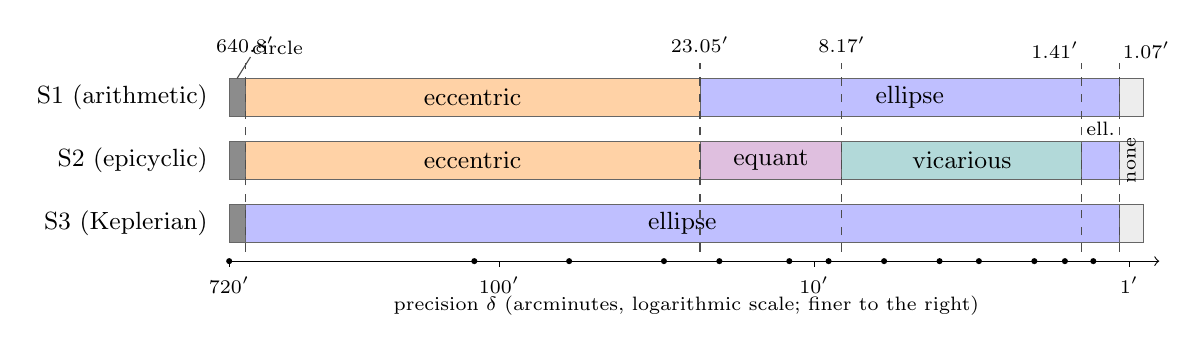
\begin{tikzpicture}[x=1cm,y=0.8cm,font=\small]
% x = 4 log10(720/delta); switch points at the minimax errors 640.79, 23.05, 8.17, 1.41, 1.07 (arcmin)
\def\keplerxc{0.202}\def\keplerxe{5.979}\def\keplerxq{7.781}\def\keplerxv{10.829}\def\keplerxl{11.306}\def\keplerxr{11.612}
\tikzset{keplerbar/.style={draw=black!60,line width=0.3pt}}
\foreach \y/\lab in {2/{S1 (arithmetic)},1/{S2 (epicyclic)},0/{S3 (Keplerian)}}{
  \node[anchor=east,font=\small] at (-0.15,\y) {\lab};
  \fill[black!7,keplerbar] (\keplerxl,\y-0.3) rectangle (\keplerxr,\y+0.3);
  \fill[black!45,keplerbar] (0,\y-0.3) rectangle (\keplerxc,\y+0.3);
}
% S1
\fill[orange!35,keplerbar] (\keplerxc,1.7) rectangle (\keplerxe,2.3); \node at ({(\keplerxc+\keplerxe)/2},2) {eccentric};
\fill[blue!25,keplerbar] (\keplerxe,1.7) rectangle (\keplerxl,2.3); \node at ({(\keplerxe+\keplerxl)/2},2) {ellipse};
% S2
\fill[orange!35,keplerbar] (\keplerxc,0.7) rectangle (\keplerxe,1.3); \node at ({(\keplerxc+\keplerxe)/2},1) {eccentric};
\fill[violet!25,keplerbar] (\keplerxe,0.7) rectangle (\keplerxq,1.3); \node at ({(\keplerxe+\keplerxq)/2},1) {equant};
\fill[teal!30,keplerbar] (\keplerxq,0.7) rectangle (\keplerxv,1.3); \node at ({(\keplerxq+\keplerxv)/2},1) {vicarious};
\fill[blue!25,keplerbar] (\keplerxv,0.7) rectangle (\keplerxl,1.3);
% S3
\fill[blue!25,keplerbar] (\keplerxc,-0.3) rectangle (\keplerxl,0.3); \node at ({(\keplerxc+\keplerxl)/2},0) {ellipse};
% thresholds
\foreach \x in {\keplerxc,\keplerxe,\keplerxq,\keplerxv,\keplerxl}{\draw[dashed,black!70] (\x,-0.45) -- (\x,2.55);}
\node[anchor=south,font=\scriptsize] at (\keplerxc,2.55) {$640.8'$};
\node[anchor=south,font=\scriptsize] at (\keplerxe,2.55) {$23.05'$};
\node[anchor=south,font=\scriptsize] at (\keplerxq,2.55) {$8.17'$};
\node[anchor=south east,font=\scriptsize,inner sep=1pt] at (\keplerxv,2.57) {$1.41'$};
\node[anchor=south west,font=\scriptsize,inner sep=1pt] at (\keplerxl,2.57) {$1.07'$};
% labels for the narrow segments
\node[anchor=south west,font=\scriptsize,inner sep=1pt] at (0.25,2.62) {circle};
\draw[black!70] (0.27,2.64) -- (0.1,2.3);
\node[font=\scriptsize] at ({(\keplerxv+\keplerxl)/2},1.5) {ell.};
\node[font=\scriptsize,rotate=90] at ({(\keplerxl+\keplerxr)/2},1) {none};
% axis
\draw[->] (0,-0.6) -- (\keplerxr+0.2,-0.6);
\foreach \x/\l in {0/720',3.429/100',7.429/10',11.429/1'}{\draw (\x,-0.6) -- (\x,-0.7) node[below,font=\scriptsize] {$\l$};}
\foreach \x in {0,3.113,4.317,5.521,6.225,7.113,7.612,8.317,9.021,9.521,10.225,10.613,10.974}{\fill (\x,-0.6) circle (1.1pt);}
\node[font=\scriptsize] at ({\keplerxr/2},-1.3) {precision $\delta$ (arcminutes, logarithmic scale; finer to the right)};
\end{tikzpicture}
\caption{The MAP form of the proof-requiring posterior over the Mars pool against the precision $\delta$ of the data, in the three syntaxes, in the noise-free common-tolerance regime (tolerances against plan94). Dashed lines: the minimax errors of \cref{tab:kepler:minimax}, below which a form is incompatible with the data; below $1.07'$ no form in the pool is compatible. Dots: the precisions at which the posterior was computed; at each of them the runner-up has at most $2^{-12.4}$ of the MAP's weight. Between dots each switch is drawn at the minimax error of the form that drops out; that form stops being the MAP somewhere between this line and the nearest dot to its left.}\label{fig:kepler:map}
\status{computed}\src{philosophy \S4.4 Part A (MAP table)}
\end{figure}

\paragraph{What the data decide and what the syntax decides} (\cref{tab:kepler:map,fig:kepler:map}). (i)~\emph{The data decide compatibility:} as $\delta$ falls the forms drop out in the historical order, circle, eccentric, equant, vicarious hypothesis, ellipse, in every syntax, as one expects, since each successor was adopted because it fitted better. (ii)~\emph{Among compatible forms the data contribute only the Occam factors, which on their own point weakly to the true form:} with a uniform prior over the five forms and no text prior, the MAP is the ellipse at every $\delta\le60'$, by $0.20$ to $14.61$ bits. (iii)~\emph{The text prior decides the rest:} law-text differences are $100$--$800$ bits for every pair of forms except one, the epicyclic syntax's equant and vicarious texts, $18$ bits apart, where the Occam factors move the margin by up to $5.6$ bits, so the text still decides. (In S1 and S3 these two texts have equal length, but both lose to the ellipse by more than $400$ bits.) So in the noise-free common-tolerance regime the syntax sets the sequence of preferred theories: with epicyclic primitives the posterior runs through every form in the historical order, switching only when a form becomes incompatible; with plain arithmetic it goes from the eccentric to the ellipse at $23'$; with a Keplerian primitive, from the circle to the ellipse at $641'$. A variable-length numeral code, Polish notation for the texts, or a natural form outside the pool changes no MAP form (\cref{sec:kepler:pooldetails}).

``The simplest theory compatible with the data'' is thus, in this regime, relative to the language of the law texts. The universal prior bounds this relativity by the cost $K(\tau)$ of a faithful translation (\cref{thm:basic:translation}), but that cost, here the definitions of the extra primitives in S1, is a few hundred bits (an estimate), as large as the text differences. Best-system accounts of laws face the same relativity (Lewis treats it as a problem and requires natural properties \citep{lewis1983new}; Cohen and Callender accept relativity to a chosen set of kinds \citep{cohen2009better}); the relation is an analogy, since best systems are a metaphysics of laws and \SAIabbr is inference from finite data. And the noise-free regime is special: a form proves all the data or none, so the power of the data to discriminate among compatible forms does not grow with their number.

\begin{example}[graded fit; a computation]\label{ex:kepler:graded}
\status{computed (the honest-band crossovers are estimates from the pricing of section 9)}\src{philosophy \S4.4 Part A'}
Under dithered rounding every form in the pool, the ellipse included, is eventually refuted (\cref{prop:laws:rounding}); but inside $\MA$ a theory may be a sampler, the law with a Gaussian error model of stated $\sigma$ (\cref{prop:laws:randomised}). At $\sigma=2'$, roughly Tycho's precision, the expected penalty per independent observation relative to the ellipse is $45.05$ bits (eccentric), $4.96$ (equant) and $0.035$ (vicarious hypothesis), so the text advantages over the ellipse are overcome after $2$ and $7$ observations (eccentric, S1 and S2), $41$ (equant, S2) and about $5{,}300$ (vicarious hypothesis, S2); a simulation agrees. Honest uniform-tolerance theories give $23$ to $71$ and about $470$ data, a conservative estimate, since \SAIabbr's mixture prefers a law with a calibrated error model (\cref{prop:laws:errormodel}; \cref{sec:kepler:gradeddetails}). So with graded fit the data, not the syntax, decide every step within tens of observations, except the epicyclic syntax's choice between the vicarious hypothesis and the ellipse on longitudes, which needs thousands of longitudes at Tycho-level noise.
\end{example}

\paragraph{Distances as data} decide that last step. Add for every day the sentence ``$r(t_i)$ lies within a factor $1\pm\tau_{\rm d}$ of $r_i$'' ($r_i$ the plan94 distance), and give each form one more element, its scale. At $\tau_{\rm d}=1\%$ the least longitude tolerance at which the vicarious hypothesis fits all the data is at most $5.12'$ (witnessed by elements; two independent searches found nothing lower), while the ellipse fits both kinds of data at $1.07'$ (\cref{tab:kepler:distances} in \cref{sec:kepler:distdetails}). So for $\delta$ below the former only the ellipse is compatible, in every syntax; with longitudes alone, only below $1.41'$. Compatibility alone thus eliminates the circle-based vicarious hypothesis once the data language contains distances: this reproduces the abandonment of circular orbits, not Kepler's last step from an oval to the ellipse, which is outside the pool. Lower bounds on the least tolerances and Occam factors with distance data were not computed.

% ------------------------------------------------------------------
\subsection{What Newton adds}\label{sec:kepler:newton}
\status{assessment, with computed figures and literature}\src{philosophy \S4.5}

Newton's theory adds masses, the constant $G$ and accelerations, with the law $m_b\ddot{\mathbf r}_b=\sum_{b'\ne b}Gm_bm_{b'}(\mathbf r_{b'}-\mathbf r_b)/\lvert\mathbf r_{b'}-\mathbf r_b\rvert^3$; the data language is unchanged (step 3 of the ladder of \cref{sec:phil:map}), and masses are theoretical in Sneed's sense, measurable only by using the theory \citep{sneed1971logical,balzer1987architectonic}. Most of what follows is the achievement of Newtonian mechanics over about 150 years, from Newton to Laplace and Le Verrier, not of Newton alone (Newton, for instance, accounted for about half of the motion of the lunar apsides, and Clairaut for the rest in 1749 \citep{nauenberg2015reception,bodenmann2010battle}). We see five points. (1)~\emph{No gain in parameters or in fit on the old data:} per body six initial conditions, as for Kepler, plus a mass, and a much longer law; on planetary longitudes at the precision of Kepler's data the extra parameters buy nothing measurable over 20 years (the ellipse fits Mars to $1.07'$), so we think that an \SAIabbr posterior on such data alone would not prefer Newton's theory (consistently with \cref{ex:kepler:graded}). (2)~\emph{Unification across domains,} where the gain lies: one law covers the planets, the Moon (the Moon test), falling bodies, tides, comets and satellite systems, and gives the third law the mass-dependent constant $q=1+m/M$ of the two-body form $(2\pi/P)^2a^3=G(M+m)$, which Jupiter's fitted $q$ matches; Saturn's deviation is accounted for by the orbit-averaged pull of Jupiter, acting like an interior ring (a heuristic estimate gives $q=1.00154$). Some of these domains need more base vocabulary. (3)~\emph{Corrections inside the old domain:} in the classical decomposition \citep{clemence1947relativity}, as given by secondary sources, Newtonian planetary perturbations account for about $531''$ of the fixed-frame advance of Mercury's perihelion, about $574''$ per century ($575.4''$ in our fits to plan94), and the remaining $43''$ or so is the effect of general relativity; Laplace explained the great inequality of Jupiter and Saturn \citep{wilson1985great}, of period about 900 years. (4)~\emph{New questions:} in the old language, where Neptune is (Le Verrier's prediction from the residuals of Uranus, also a standard example of reference fixed by a description \citep{kripke1980naming}); in a new language, the masses of the Sun and of the planets with satellites. (5)~\emph{No deductive entailment:} Newton's axioms do not entail $\mathrm{K12}$ or $\mathrm{K3}$, and with the planets' masses they contradict their exact form, as \citet{duhem1954aim} observed; with masses and initial conditions they entail honest tolerance forms, ``$\mathrm{K12}$ holds within $\varepsilon(b,W)$ on the window $W$'' (\cref{prop:laws:correction} is a provable toy version). A formal derivation of even one such bound needs an existence-and-uniqueness theorem and a validated integration or perturbation estimate, a very long derivation that no textbook writes out: a concrete case of the computational gap between a written theory and the reasoner who uses it (\cref{sec:limits:textbook}).

% STUB written by the planning editor. The section writer replaces this file.
% Plan: ../OUTLINE.md (section "sec:limits"); results: ../CLAIMS.md; notation: ../NOTATION.md.
\section{Limitations}\label{sec:limits}
\emph{(To be written.)}

% STUB written by the planning editor. The section writer replaces this file.
% Plan: ../OUTLINE.md (section "sec:related"); results: ../CLAIMS.md; notation: ../NOTATION.md.
\section{Related work}\label{sec:related}
\emph{(To be written.)}

% Discussion, open problems, acknowledgements, code and data (front writer). Plan: ../OUTLINE.md "§13 Discussion";
% synthesis research/notes-final.md §0 (philosophy paragraph), §2.7 (verdict), §2.8, §6 (open problems; the five starred ones
% are named first), §8.6 (re-runs, for the Code and data statement); CLAIMS.md §12 (every q: label is cited below).
% Acknowledgements as in the companion papers (DECISIONS §A4, REFRAME §4); the body uses no work of S. Eisenstat or
% D. Vaintrob, so they are not thanked here. Author decision (2026-10-17): the sentence "Hänni takes responsibility for the content of this paper" is removed now that the paper has two authors; do not reinstate it.
% Edit pass of 2026-10-17 (review/DECISIONS.md; FRO-13 to FRO-16, FRO-19, FRO-L2): U1 (long form, first sentence shortened as
% allowed), U2 (discussion version), U3 (first sentence); FRO-14, FRO-15; acknowledgements without the sentence that repeated the
% title-page footnote; list A and list B of DECISIONS §L3 (front, §13). The Code and data sentence on the README stays (FRO-19):
% the README is a blocking item of the publication step (DECISIONS §X9).

\section{Discussion}\label{sec:discussion}

\paragraph{What the formalism shows.} \SAI makes precise the view that theories answer questions posed in a given language, and the view survives in comparative form: it changes the target, the data type, logical coherence and partiality (\cref{sec:phil:questions,tab:phil:differences}), while the inference principle is unchanged: version by version and up to constant factors, \SAIabbr agrees with operator induction over consistent labellers (\cref{sec:soi}). On data labelled true or false the idealised formalism cannot see the difference between a theory and a program. In the settings we study, shape becomes visible only when something other than program length is charged (the written theory, the time to produce it, or the derivations) or the class of hypotheses is restricted (to finite theories); there it is relative to a reasoner and a vocabulary, and for theoretical terms what pays is relations and entities, not vocabulary as such. Whether this holds beyond these settings is open (\cref{q:shape:beyond}). That textbook theories are declarative is an observation we accept, and we find it plausible that this shape is good, but in our models declarative against procedural form buys at most a constant factor once intermediate concepts are available and the reasoner can chain through them; what is missing is a formal setting in which that shape provably pays. Finally, ``Kepler's laws are only approximately true'' is a limitation of proof-requiring compatibility with deterministic theories, not of the axiom view as \SAIabbr formalises it: its mixture contains randomised theories, and under its pricing an approximately true law is a law with a calibrated error model (\cref{prop:laws:errormodel}).

\paragraph{What it cannot show.} The axiom view models the declarative core of scientific theories (contents, inferential relations, partiality, approximate truth) and misses their procedural, statistical and dynamic sides (\cref{sec:limits}). It supports no general realist conclusion about the theories it favours: it identifies a complete r.e.\ theory that the data present (\cref{prop:basic:limits}), but its limit posterior can live on random theories and, with adversarially chosen true data, on false ones (\cref{thm:logic:lottery,cor:logic:false}). It evaluates theories and does not find them, and it is not computable.

\subsection{Open problems}\label{sec:discussion:open}

\begin{enumerate}[leftmargin=*,label=(\arabic*)]
\item Does $\MA$ dominate every lower semicomputable provability function of a random consistent theory (\cref{q:basic:domination})?
\item Is there a stream with bounded one-tape loss on which the coin-free loss diverges computably fast, and does bounded one-tape loss on a co-r.e.\ stream imply that a consistent r.e.\ theory proves it (\cref{q:logic:computablefast})?
\item Over a true background containing $\PA$, is the one-tape posterior probability of $\Sigma_1$-soundness bounded away from $1$ uniformly over all data (\cref{q:logic:soundness})?
\item Does the dependence of written size on the pair (reasoner, vocabulary) extend beyond Boolean laws, to real-valued laws with numerical solvers, probabilistic programs with conditioning and simulation codes (\cref{q:shape:beyond})?
\item Is there a formal setting for communities of bounded reasoners who communicate, check and extend theories piece by piece, in which theories of declarative shape provably do better than programs (\cref{q:phil:declarative})?
\end{enumerate}
The further questions are \cref{q:basic:tape,q:basic:indeporder,q:soi:lsc,q:soi:pathwise,q:soi:presburger,q:logic:soundtrue,q:logic:codingO1,q:logic:thn,q:logic:kreisel,q:terms:binaryobs,q:terms:a1,q:terms:unaryfunction,q:shape:minimum,q:shape:learning,q:shape:cellprobe,q:laws:JR,q:laws:domains}.

\paragraph{Directions.} The directions we find most worth pursuing are step 4 of the ladder, for which we have no formal handle; the setting of problem (5), where the declarative shape of written theories may find its explanation; a costed-deduction mixture over unknown axiom systems, combining \SAIabbr, uncertain about the axioms, with logical induction \citep{garrabrant2016logical}, uncertain about their consequences, as induction in mathematics needs (\cref{prop:logic:oldevidence}); and a native treatment of statistical confrontation inside the proof-requiring core (\cref{sec:limits:stat}). Smaller ones: whether explanatory asymmetry is interventional in general, and a derivation of Kepler's laws within stated tolerances from Newton's theory in a prover for validated numerics (\cref{sec:limits:textbook}).

\section*{Acknowledgements}\addcontentsline{toc}{section}{Acknowledgements}
Several of the questions and examples studied here first appeared in H\"anni's working notes \citep{hanni2026notes}. The results of our earlier report \citep{claude2026axiominduction} and of the companion papers \citep{claudeSFI2026fundamentals,claudeSFI2026steeper} that we use were prepared and checked in the same way as this paper. No human has yet independently checked all of the mathematics, and nothing was verified in a proof assistant; readers should weigh the results accordingly.

\section*{Code and data}\addcontentsline{toc}{section}{Code and data}
All computations reported here were done with seeded or deterministic Python scripts (Python~3.11 with NumPy, SciPy and mpmath; the planetary computations use pyerfa, the Python interface to the ERFA library). The scripts, their saved outputs and independent re-implementations of the main computations are in the folder \texttt{solomonoff-axiom-induction/} of the repository \url{https://github.com/kaarelh/AI-works}; its README lists the script behind each reported number and how to re-run it. Re-running the scripts reproduces the saved outputs, apart from lines that report run times; the longest computations, on the Mars pool, take more than half an hour each, and their figures were also reproduced by independent re-implementations.


\bibliographystyle{plainnat}
\bibliography{bib/all}

\appendix
% STUB written by the planning editor. The section writer replaces this file.
% Plan: ../OUTLINE.md (section "app:basic"); results: ../CLAIMS.md; notation: ../NOTATION.md.
\section{Proofs for the setting and the basic theorems}\label{app:basic}
\emph{(To be written.)}

% STUB written by the planning editor. The section writer replaces this file.
% Plan: ../OUTLINE.md (section "app:soi"); results: ../CLAIMS.md; notation: ../NOTATION.md.
\section{Proofs for the relation to operator induction}\label{app:soi}
\emph{(To be written.)}

% STUB written by the planning editor. The section writer replaces this file.
% Plan: ../OUTLINE.md (section "app:logic"); results: ../CLAIMS.md; notation: ../NOTATION.md.
\section{Proofs for random theories, \texorpdfstring{$\Pi_1$}{Pi1} data and G\"odel phenomena}\label{app:logic}
\emph{(To be written.)}

% STUB written by the planning editor. The section writer replaces this file.
% Plan: ../OUTLINE.md (section "app:phil"); results: ../CLAIMS.md; notation: ../NOTATION.md.
\section{Proofs for what a theory does and is}\label{app:phil}
\emph{(To be written.)}

% STUB written by the planning editor. The section writer replaces this file.
% Plan: ../OUTLINE.md (section "app:shape"); results: ../CLAIMS.md; notation: ../NOTATION.md.
\section{Proofs for theory shape}\label{app:shape}
\emph{(To be written.)}

% STUB written by the planning editor. The section writer replaces this file.
% Plan: ../OUTLINE.md (section "app:terms"); results: ../CLAIMS.md; notation: ../NOTATION.md.
\section{Proofs for theoretical terms}\label{app:terms}
\emph{(To be written.)}

% Appendix G: proofs for approximate laws and the best system (owner: laws group).
% Plan: ../OUTLINE.md (app:laws); rows: ../CLAIMS.md section 8; notation: ../NOTATION.md section 8.1.
% Full statements of the results that sec:laws states in words, and the proofs of all results of sec:laws.
% Local symbols (renamed from the source items, NOTATION section 11 and local choices):
%   c_time (pi_c); zeta_j (eta_j); patch set Z (S); \underline f,\overline f (l,u); \mathcal G, \mathcal F (G, F);
%   band position w (x); boundary position v (V); \vartheta (phi of Lemma 3.6); \bar c_\Delta(w) (C_Delta(w));
%   P^\star (true conditional law P); level x, times tau_x, varsigma_x (L, tau_L, sigma_L of Thm 3.8);
%   map Psi (F of section 4), dimension m (d), propagated tolerance \varepsilon^{(r)} (e_r);
%   T_tr, h_tr (N, h_N); system \star (M); \mathrm{El}_b (E_b); literal cost gamma (c); n_tot (N);
%   Rot, \mathbf P, \eta_c, \bar t, T_new (R, P, eta, W, T_N); Pt_f, Pt_s, Cop (P_f, P_s, C);
%   \theta_{sh}, k_{sh} (C, k_C); Act (Lewis's F); module lengths ||.|| without stop bit.
\section{Proofs for approximate laws and the best system}\label{app:laws}

This appendix states in full the results of \cref{sec:laws} that the main text states in words, and proves every result of that section. The notation is that of \cref{def:laws:setting}. We measure a finite theory by $\lVert T\rVert$, without the stop bit of a prefix-free code of theories; using the prefix-free length $\lVert T\rVert+1$ instead changes every statement below by an additive constant at most, and shifts $J_\lambda$ by the same amount $\lambda$ on every theory, so that it leaves the $\lambda$-MAPs unchanged. Computed numbers come from seeded scripts in the accompanying repository; they are never part of a statement.

\subsection{The setting in full}\label{app:laws:setting}

\paragraph{Technical points.} (i) \emph{Rational cells.} In regime R the dither $u_j$ is uniform on a grid $\{k/N_{\rm d}:0\le k<N_{\rm d}\}$, so that cell endpoints are rational. Every event used below has the form ``$u_j$ lies in an interval of length $\ell'$'', whose grid probability is within $1/N_{\rm d}$ of $\ell'$; the formulas are the limit $N_{\rm d}\to\infty$ (equivalently, endpoints may be real algebraic numbers). A cell that crosses the zero point of the circle is a disjunction of two interval sentences. (ii) \emph{Fresh times.} Data are sentences, so they mention numerals, a countable set; no atomless law lives on it. Times drawn i.i.d.\ from a law on numerals repeat: the number of distinct times among $n$ draws is $o(n)$ almost surely (take a finite set of mass at least $1-\epsilon$ and apply the strong law of large numbers). A repeat changes the cost of every form except an exact law: a patched law withdraws the law at a whole time, so every later datum at a refuted time is an exception, and the cells of an honest law at one time intersect, which narrows its band. A computation with times drawn uniformly from the $4383$ days of a twelve-year window (sinusoidal error, $\varepsilon^*=1'$, $\Delta=60'$, $\lambda=1$, $c_{\rm time}=\log4383+2$) gives a patched law's cost per datum of $0.40$, $1.96$ and $3.23$ bits at $n=10^3$, $10^5$ and $2\times10^5$, against the rate $0.240$ at fresh times, and a code-R cost of the honest law falling from $0.037$ to $0.022$, against $0.030$. This is why regime R takes fresh times: an injective computable sequence of numerals, with i.i.d.\ errors and dithers. Fresh times have names that grow, and \cref{prop:laws:patches} says what that costs. (iii) \emph{Presentations.} No decidable set of programs covers all total computable maps, so the class of pointwise interval laws depends on the presentation language (for example, primitive recursive definitions, or programs paired with an explicit clock); every statement holds for each fixed choice. (iv) \emph{A model of the data.} In regime R the error at a fresh time is a draw from a fixed law; for the Kepler residuals this law is the law of $e(t)$ for $t$ uniform in the window. Answered data with a question $\mathcal Q$ are read through \cref{def:setting:questions}: for consistent $B\cup T$, $T$ proves $(\mathcal Q,a)$ iff $A_T(\mathcal Q)=\{a\}$, since $T\vdash a$ refutes every other answer by incompatibility, and refuting every other answer proves $a$ because $B$ proves $\bigvee\mathcal Q$.

\begin{lemma}[Decidability]\status{proved}\src{laws Lemma 1.6}\label{lem:laws:decidable}
Let $T$ be a pointwise interval law and $C$ a cell, a finite union of intervals with rational endpoints. Then $T$ proves the datum ``$q_t\in C$'' iff $[\underline f(t),\overline f(t)]\subseteq C$, and refutes it iff $[\underline f(t),\overline f(t)]\cap C=\emptyset$; and $B\cup T\cup D^\pm$ is consistent iff, for every time $t$ of $D$, $[\underline f(t),\overline f(t)]$ meets the intersection $C_t$ of the cells that $D$ assigns to $t$. All three are decidable from the presentation of $T$.
\end{lemma}

\begin{proof}
Every choice of reals $q_t\in[\underline f(t),\overline f(t)]$ gives a model of $B\cup T$ in $\mathbb R$, and if the $q_t$ also lie in the assigned cells, a model of $B\cup T\cup D^\pm$. This gives the ``only if'' of the first two claims (choose $q_t$ outside the cell, respectively inside it) and the ``if'' of the third. Inclusion and disjointness of finite unions of rational intervals are Boolean combinations of inequalities between rational numerals, which $\mathrm{RCF}$ proves or refutes; this gives the ``if'' of the first two claims. If for some $t$ the interval misses $C_t$, the finitely many inequalities involved are jointly refutable in $\mathrm{RCF}$, which gives the ``only if'' of the third. The values $\underline f(t),\overline f(t)$ are computable from the presentation, so all three conditions are decidable.
\end{proof}

\begin{proposition}[Laws plus listed exceptions are deterministic hypotheses]\status{proved}\src{laws Prop 1.4}\label{prop:laws:exceptions}
\leavevmode
\begin{enumerate}[label=(\alph*),itemsep=1pt,topsep=2pt]
\item For every finite $T$ with $B\cup T\cup D^\pm$ consistent, $\LA(D)-c\le\KA(D)\le\lVert T\rVert+\Exc^F_D(T)+c$.
\item For an r.e.\ $T$ and $E\subseteq D$ with $B\cup T\cup E^\pm$ consistent and $B\cup T\cup E^\pm\vdash\psi_D$, $\LA(D)\le\Keq(T)+K(E)+c$.
\end{enumerate}
\end{proposition}

\begin{proof}
(a) The finite set $T':=T\cup\{a:(\mathcal Q,a)\text{ a datum of $D$ that $T$ does not prove}\}$ is contained in the consistent set $T\cup D^\pm$, so $B\cup T'$ is consistent, and $T'$ proves every datum. Concatenating the codewords of the sentences of $T$, each after a continuation bit, the codewords $c_S(a)$ of the exceptions, each after a continuation bit, and a stop bit gives a prefix-free code of $T'$ of length $\lVert T\rVert+\Exc^F_D(T)+1$, and a fixed program turns it into an index of $T'$. So $\KA(D)\le\lVert T\rVert+\Exc^F_D(T)+c$. The instance form of dominance (\cref{thm:basic:dominance}) gives $\MA(D)\ge2^{-K(e)-c}$ for every index $e$ of a theory consistent with $B$ that proves $\psi_D$, hence $\LA(D)\le\KA(D)+c$. (b) is \cref{prop:basic:exceptions}(b).
\end{proof}

So code F pays for \emph{which} questions are exceptions, since the answer sentence names its question; a deterministic theory cannot avoid this, because it does not see the questions.

\subsection{Randomised theories and the best two-part code}\label{app:laws:random}

\begin{proposition}[Randomised theories pay question-relative costs]\status{proved}\src{laws Prop 1.8}\label{prop:laws:randomised}
Let $T$ be a pointwise interval law and $D$ a set of interval data consistent with $T$.
\begin{enumerate}[label=(\alph*),itemsep=1pt,topsep=2pt]
\item $\LA(D)\le K(T)+\Exc^R_D(T)+c\le\lVert T\rVert+\Exc^R_D(T)+c$.
\item If $D$ comes from a computable question family with one question $\mathcal Q_t$ per time, and $k_t(T):=\lvert A_T(\mathcal Q_t)\rvert\le\lvert\mathcal Q_t\rvert$, then $\LA(D)\le K(T,(\mathcal Q_t)_t)+\sum\log k_t(T)+c$, the sum over the data that $T$ does not prove; in particular $\LA(D)\le K(T,(\mathcal Q_t)_t)+\Exc^Q_D(T)+c$.
\item Code R charges an exception of a patched law, at a time where $\underline f=0$ and $\overline f=\mathsf R$, exactly $\log(\mathsf R/\lvert C_t\rvert)$, which is the code-Q cost for equal cells; it charges the honest law $-\log(\lvert C_t\cap[f(t)-\varepsilon,f(t)+\varepsilon]\rvert/2\varepsilon)$, which is $0$ when the band lies inside the cell.
\end{enumerate}
\end{proposition}

\begin{proof}
(a) \emph{The machine.} Enumerate $I$ as $t_1,t_2,\dots$ and fix a computable injection $(i,k)\mapsto\langle i,k\rangle$ into tape positions, increasing in $k$. On a tape $\omega$ put $U_i:=\sum_{k\ge1}\omega_{\langle i,k\rangle}2^{-k}$; under $\Unif$ the $U_i$ are independent and uniform on $[0,1]$. Let $G_T$ be the theory machine that emits the sentences of $T$ at the empty prefix and, once the prefix read contains the positions $\langle i,1\rangle,\dots,\langle i,k\rangle$, whose bits form the binary numeral of an integer $m$, also emits
\[\underline f(t_i)+(\overline f-\underline f)(t_i)\,m2^{-k}\ \le\ q_{t_i}\ \le\ \underline f(t_i)+(\overline f-\underline f)(t_i)\,(m+1)2^{-k}.\]
This set of (prefix, sentence) pairs is c.e., and an index of it is computable from the presentation of $T$, so $K(G_T)\le K(T)+c$.

\emph{The random theory is always consistent.} Put $q_{t_i}:=v_i:=\underline f(t_i)+(\overline f-\underline f)(t_i)U_i$. Each emitted closed interval contains $v_i$, so these values satisfy every emitted sentence, and $\mathbb R$ with them is a model.

\emph{It proves a datum ``$q_{t_i}\in C$'' whenever $v_i$ lies in the interior of $C$.} The emitted intervals contain $v_i$ and have lengths $(\overline f-\underline f)(t_i)2^{-k}\to0$, so one of them lies in the interior of $C$, and $\mathrm{RCF}$ proves the inclusion. (If $\underline f(t_i)=\overline f(t_i)$, $T$ alone decides the datum.) The times of $D$ are distinct indices $i$, the $U_i$ are independent, and endpoints have probability $0$, so
\[\nu_{G_T}(D)\ \ge\ \Unif\{\omega:v_t\in\operatorname{int}C_t\text{ for every time $t$ of $D$}\}\ =\ P^R_T(D).\]
Dominance (\cref{thm:basic:dominance}), $\MA\ge2^{-K(\nu)}\nu$ for every theory-machine law $\nu$, gives $\MA(D)\ge2^{-K(G_T)-c}\nu_{G_T}(D)$, which is (a); and $K(T)\le\lVert T\rVert+c$.

(b) Let the machine use $U_i$ to pick the $\lfloor k_{t_i}(T)U_i\rfloor$-th element $a$ of $A_T(\mathcal Q_{t_i})$, which is computable by \cref{lem:laws:decidable}, and emit $a$ as soon as enough bits have been read (almost surely after finitely many). The cell $a$ meets $[\underline f(t_i),\overline f(t_i)]$, so the random theory has a model in $\mathbb R$; it proves the true answer with probability $1/k_{t_i}(T)$, independently across times, and $k_t(T)=1$ when $T$ proves the datum. Since $D$ is consistent with $T$, $T$ refutes no datum. The machine's index is computable from $T$ and the question family, and dominance gives the bound; the last claim follows from $\log k_t(T)\le\log\lvert\mathcal Q_t\rvert=\gamma(\mathcal Q_t)$. (c) is the definition of $P^R_T$.
\end{proof}

\begin{proposition}[\SAIabbr is the best two-part code over theory machines]\status{proved, given thm:basic:dominance, rem:terms:named, thm:basic:nocoding and Proposition 5.7 of the companion paper on steeper priors}\src{laws Prop 1.9}\label{prop:laws:twopart}
\leavevmode
\begin{enumerate}[label=(\alph*),itemsep=1pt,topsep=2pt]
\item For every data set $D$, $\LA(D)=\min_G[K(G)-\log\nu_G(D)]\pm c$, the minimum over theory machines $G$; it is attained, up to $c$, by $G_U$.
\item Restricting $G$ gives upper bounds: $\LA(D)\le\min_TJ^R_1(T;D)+c$ over pointwise interval laws, $\LA(D)\le\min_TJ^F_1(T;D)+c$ over finite theories, and $\LA(D)\le\KA(D)+c$.
\item Neither $\KA$ nor $\min_TJ^Q_1(T;\cdot)$ over finite theories is within an additive constant of $\LA$ in general; nor, therefore, is $\min_TJ^F_1(T;\cdot)$ when $\gamma\le\ell$.
\item Over all theory machines steeper selection collapses. Take the point family of programs $p\in\dom V$ for theory machines, with length $\lvert p\rvert$ and fit $-\log\nu_{G_{V(p)}}(D)$, and let $\ell_U$ be the length of a program for $G_U$. For $\lambda>1$, every $\lambda$-MAP $p$ has $\lvert p\rvert\le\ell_U+\ell_U/(\lambda-1)$.
\end{enumerate}
\end{proposition}

\begin{proof}
(a) Dominance gives $\LA(D)\le K(G)-\log\nu_G(D)+c$ for every theory machine $G$, and $\MA=\nu_{G_U}$ gives $K(G_U)-\log\nu_{G_U}(D)=\LA(D)+O(1)$. (b) is \cref{prop:laws:exceptions,prop:laws:randomised} with $\Keq$ and $K$ of a finite theory at most its length plus a constant.

(c) That $\KA-\LA$ is unbounded is the absence of a coding theorem (\cref{thm:basic:nocoding}). For $\min_TJ^Q_1(T;\cdot)$, take the language $\{R\}\cup\{c_j:j\in\mathbb N\}$ with $B=\emptyset$ and the yes/no data $D_n:=\{(R(c_j),1):j<n\}\cup\{(\exists x\,\neg R(x),1)\}$, so that every datum has literal cost $\gamma=1$. By \cref{rem:terms:named}, applied to the r.e.\ theory $\{R(c_j):j\in\mathbb N\}\cup\{\exists x\,\neg R(x)\}$, $\KA(D_n)\le c$, hence $\LA(D_n)\le\KA(D_n)+c\le c'$. Let $T$ be finite with $B\cup T\cup D_n^\pm$ consistent. If $c_j$ does not occur in $T$ and $T\vdash R(c_j)$, then $T\vdash\forall x\,R(x)$ by the theorem on constants, which contradicts consistency with $\exists x\,\neg R(x)$. So $T$ proves at most the data $R(c_j)$ with $c_j$ occurring in $T$, together with $\exists x\,\neg R(x)$. In a syntax code in which each symbol occurrence costs at least one bit, each constant occurring in $T$ costs at least one bit of $\lVert T\rVert$, and each unproved datum one bit of $\Exc^Q$; so $J^Q_1(T;D_n)\ge n$. Finally $\Exc^F\ge\Exc^Q$ when $\gamma\le\ell$, since then each exception costs at least as much in code F.

(d) \citet[Proposition~5.7(ii)]{claudeSFI2026steeper} states: if a point family contains a member $\pi_U$, of length $\ell_U$, with fit $L(\pi_U)\le L(\pi)+\ell(\pi)+\kappa_0$ for every member $\pi$, then for every $\lambda>1$ every $\lambda$-MAP has length at most $\ell_U+(\ell_U+\kappa_0)/(\lambda-1)$. The mixture identity of \cref{thm:basic:dominance} gives $\MA(D)\ge\sum_{p\in\dom V}2^{-\lvert p\rvert}\nu_{G_{V(p)}}(D)\ge2^{-\lvert p\rvert}\nu_{G_{V(p)}}(D)$ for each $p$, so a program $p_U$ for $G_U$ has fit $-\log\nu_{G_U}(D)=\LA(D)\le-\log\nu_{G_{V(p)}}(D)+\lvert p\rvert$ for every $p$. This is the hypothesis with $\kappa_0=0$.
\end{proof}

\begin{remark}[Pointwise interval laws: the separation is open]\status{proved, given prop:basic:chain and prop:laws:codingbound; open}\src{laws Rem 1.9a}\label{rem:laws:JR}
For every set $D$ of interval data, both $\LA(D)$ and $\min_TJ^R_1(T;D)$ over pointwise interval laws are at least $K(y_D\mid\dom D)-c$. For $\LA$: the answer conjunctions of the questions in $\dom D$ form a finite set $S$ of pairwise $B$-incompatible sentences, computable from $\dom D$, and $\MA(D)=\MA(\{(\psi_D,1)\})$ (\cref{prop:basic:structure}); so the coding lower bound of \cref{prop:basic:chain} gives $\LA(D)\ge K(\psi_D\mid S)-c\ge K(y_D\mid\dom D)-c'$. For $J^R_1$: \cref{prop:laws:codingbound}(b). So neither bound separates the two. The natural candidate for a separation, data in which pairs of times share a random cell, has $\LA\approx n\gamma/2$; but it does not separate them either, because a presentation may store values: the program that stores the $n/2$ shared cells and returns each for both times of its pair has length $n\gamma/2+O(\log n)$ and $\Exc^R=0$, so $\min_TJ^R_1\le n\gamma/2+O(\log n)$ as well.
\end{remark}

\begin{question}\status{open}\src{laws Rem 1.9a}\label{q:laws:JR}
Fix a presentation language for pointwise interval laws. Is $\min_TJ^R_1(T;D)-\LA(D)$ bounded over all sets $D$ of interval data? (For $\KA$ and for $\min_TJ^Q_1$ over finite theories the answer is no, by \cref{prop:laws:twopart}(c).)
\end{question}

\begin{proposition}[Which hypotheses of the companion paper on steeper priors hold here]\status{proved, given the companion paper on steeper priors}\src{laws Prop 1.10}\label{prop:laws:P2hyp}
\leavevmode
\begin{enumerate}[label=(\alph*),itemsep=1pt,topsep=2pt]
\item \emph{Pointwise interval laws in code R} (a fixed presentation language; one question family with finitely many cells). The codewords form a decidable prefix-free set; $P^R_T$ is computable uniformly in $T$, is the law $\nu_{G_T}$ of a theory machine (a shared hypothesis in the sense of \citealp[Definition~3.4]{claudeSFI2026steeper}) and, on data at distinct times, a product hypothesis \citep[Definition~3.3]{claudeSFI2026steeper}; Kraft's inequality holds, lengths are integers, and finitely many laws have each length. So Lemmas~A.1, 3.8, 3.9 and 5.3, Corollaries~5.4 and 5.5 and Theorem~5.6 of \citet{claudeSFI2026steeper} apply, with $J_\lambda=J^R_\lambda$.
\item \emph{Finite theories over a decidable consistent $B$, in code Q}, with $P_T(D):=2^{-\Exc^Q_D(T)}\ind[B\cup T\cup D^\pm\text{ consistent}]$. $P_T$ satisfies the semimeasure inequalities of \citet[Definition~3.4]{claudeSFI2026steeper}, and it is a product over questions when consistency can be checked question by question (pointwise laws at distinct times). It is not lower semicomputable in general (for $B=\emptyset$ and a language with a binary relation symbol), so this class is not a hypothesis class of the companion paper. Its hull lemma (Lemma~3.8), kink lemma (Lemma~5.3), Corollary~5.4, Theorem~5.6 and Lemma~A.1(i) use only the point family $(\lVert T\rVert,\Exc^Q_D(T))_T$ and apply. Its coding bound (Lemma~3.9) is replaced by \cref{prop:laws:codingbound}, with which Corollary~5.5 holds with offset $b+\kappa+n$ in general, and $b+\kappa$ when provability of the answers from the theories is decidable ($\kappa$ the constant of \cref{prop:laws:codingbound}).
\end{enumerate}
\end{proposition}

\begin{proof}
\emph{Which hypotheses are used.} Each listed property is checked in the statement: for (a), $P^R_T=\nu_{G_T}$ on interval data by the proof of \cref{prop:laws:randomised}(a) (the random theory proves ``$q_t\in C$'' iff $v_t\in\operatorname{int}C$, up to null events), and the product form holds because the $U_i$ are independent. That the hull, kink and converse results need only the point family can be read off their statements, which concern countable point families, and their proofs, which use only lengths, fits, and the finiteness of the set of programs of each length.

\emph{The semimeasure inequalities in (b).} $P_T(\emptyset)=\ind[B\cup T\text{ consistent}]\le1$. Let $\mathcal Q\notin\dom D$ and $P_T(D)>0$. If $T$ proves an answer $a_0$, every other answer is refuted by $T$ and contributes $0$, while $a_0$ adds no cost and keeps consistency; so the sum is $P_T(D)$. If $T$ proves no answer, each of the at most $\lvert\mathcal Q\rvert$ answers consistent with $B\cup T\cup D^\pm$ contributes at most $2^{-\gamma(\mathcal Q)}P_T(D)=P_T(D)/\lvert\mathcal Q\rvert$. If $P_T(D)=0$, every term is $0$.

\emph{Not lower semicomputable.} Take $B=\emptyset$ and a language with a binary relation symbol. If $T\mapsto P_T(\emptyset)$ were lower semicomputable uniformly in $T$, the set of finite theories with $P_T(\emptyset)>\frac12$, that is the consistent ones, would be r.e. The inconsistent ones are r.e.\ as well, so consistency of finite theories would be decidable, contrary to Church's theorem (standard; \citealp{church1936note}).
\end{proof}

\begin{proposition}[Coding bound for laws with literal exceptions]\status{proved}\src{laws Prop 1.11}\label{prop:laws:codingbound}
Let $n:=\lvert D\rvert$.
\begin{enumerate}[label=(\alph*),itemsep=1pt,topsep=2pt]
\item For every finite $T$ with $B\cup T\cup D^\pm$ consistent, $\lVert T\rVert+n+\Exc^Q_D(T)\ge K(y_D\mid\dom D)-c$.
\item Suppose that provability of answers from $T$ is decidable uniformly in $T$, for $T$ ranging over a class of presented theories with $K(T)\le\lVert T\rVert+c$ (finite theories over a decidable complete $B$, or pointwise interval laws). Then $\lVert T\rVert+\Exc^Q_D(T)\ge K(y_D\mid\dom D)-c$ and $\lVert T\rVert+\Exc^R_D(T)\ge K(y_D\mid\dom D)-c$ for every member $T$ consistent with $D$.
\end{enumerate}
\end{proposition}

\begin{proof}
(a) For a question $\mathcal Q$ put
\[w_T(a\mid\mathcal Q):=\tfrac12\ind[a\text{ is the first answer of }\mathcal Q\text{ found provable from }B\cup T]+\tfrac12\lvert\mathcal Q\rvert^{-1},\]
where ``first'' refers to a fixed dovetailed proof search. Then $\sum_aw_T(a\mid\mathcal Q)\le1$, and $w_T$ is lower semicomputable uniformly in $(T,\mathcal Q)$, because the first answer found never changes. So $P'_T(y):=\prod_jw_T(y_j\mid\mathcal Q_j)$ is a semimeasure on the answer lists for $\dom D$, lower semicomputable uniformly in $(T,\dom D)$. If $B\cup T$ is consistent and proves $y_j$, it proves no other answer of $\mathcal Q_j$, so $y_j$ is the first found and $w_T(y_j\mid\mathcal Q_j)\ge\frac12$; otherwise $w_T(y_j\mid\mathcal Q_j)\ge\frac12\lvert\mathcal Q_j\rvert^{-1}$. Hence $-\log P'_T(y_D)\le n+\Exc^Q_D(T)$. The conditional coding theorem ($K(y\mid z)\le-\log P(y\mid z)+c_P$ for a semimeasure $P(\cdot\mid z)$ lower semicomputable uniformly in $z$; standard, see \citealp{li2008introduction}) gives $K(y_D\mid T,\dom D)\le n+\Exc^Q_D(T)+c$, and $K(y_D\mid\dom D)\le K(T)+K(y_D\mid T,\dom D)+c\le\lVert T\rVert+n+\Exc^Q_D(T)+c'$.

(b) With decidable provability put $w_T(a\mid\mathcal Q):=1$ if $a$ is the first answer, in a fixed order of $\mathcal Q$, that $T$ proves; $:=0$ for the other answers that $T$ proves; and $:=\lvert\mathcal Q\rvert^{-1}$ for every answer if $T$ proves none. This sums to at most $1$ for every $T$, consistent or not, and it is computable. For $T$ consistent with $D$ the cost bound of (a) holds without the flag bit, and the same coding argument gives the first inequality. For code R, $P^R_T(\cdot\mid\dom D)$ is itself a semimeasure on answer lists, computable uniformly in $(T,\dom D)$ (\cref{prop:laws:P2hyp}(a)), and the same argument gives the second.
\end{proof}

So the right line of slope $1$ around a sufficient law \citep[Corollary~5.5(a)]{claudeSFI2026steeper} holds in both classes; in code Q without decidability it carries the flag cost $n$, which makes it useless, and for that reason the analyses of \cref{sec:laws} use laws whose provability on the data is decidable.

\subsection{Deterministic theories and precision}\label{app:laws:precision}

\begin{proposition}[Compatibility is monotone in logical strength]\status{proved}\src{laws Prop 2.1, Cor 2.2}\label{prop:laws:strength}
\leavevmode
\begin{enumerate}[label=(\alph*),itemsep=1pt,topsep=2pt]
\item Let $B\cup T$ be consistent and $\Cn(T)\supseteq\Cn(T')$. On every data set with which $T'$ is compatible ($B\cup T'$ consistent and proving every datum), $T$ is compatible. So among the deterministic hypotheses of $\WA$ and $\MA$ the posterior odds of $T$ against $T'$ equal their prior odds on every data set with which $T'$ is compatible, and $T'$ is incompatible whenever $T$ is: data never move the odds towards the weaker theory.
\item $T_0\vdash T^\varepsilon$ for every $\varepsilon\ge0$, so every data set compatible with the honest law $T^\varepsilon$ is compatible with the exact law $T_0$, at every sample size and every precision. With prior weights $2^{-\lVert T\rVert}$ in a code in which the tolerance clause costs at least one bit, the posterior odds of $T_0$ against $T^\varepsilon$ are at least $2^{\lVert T^\varepsilon\rVert-\lVert T_0\rVert}\ge2$ on every such data set.
\item If $\sup_t\lvert e(t)\rvert>0$, then $T_0$ is false and, on a question at precision $\delta'<\sup_t\lvert e(t)\rvert$, proves a false answer at some times; $T^\varepsilon$ with $\varepsilon\ge\sup_t\lvert e(t)\rvert$ is true and is silent wherever its band straddles a cell boundary.
\end{enumerate}
\end{proposition}

\begin{proof}
A consistent theory that proves everything $T'$ proves proves every datum that $T'$ proves; this is (a), and (b) is (a) with $T=T_0$, $T'=T^\varepsilon$. (c) is immediate from the definitions.
\end{proof}

\begin{proposition}[Precision monotonicity]\status{proved}\src{laws Prop 2.3}\label{prop:laws:monotone}
If $B\cup T$ proves ``$q(t)\in[v-\delta',v+\delta']$'', then it proves ``$q(t)\in[v-\delta,v+\delta]$'' for every $\delta\ge\delta'$. So compatibility with data at a fixed set of centres is monotone in the precision.
\end{proposition}

\begin{proof}
The first interval is contained in the second.
\end{proof}

\begin{proposition}[Guaranteed tolerances]\status{proved; computed}\src{laws Prop 2.4}\label{prop:laws:tolerance}
In regime G:
\begin{enumerate}[label=(\alph*),itemsep=1pt,topsep=2pt]
\item $T_0$ proves datum $j$ iff $\lvert e(t_j)-\zeta_j\rvert\le\delta$, and refutes it otherwise.
\item If $\delta\ge\varepsilon^*+\delta_0$, then $T_0$ is compatible, at every $n$, with every such data set whose errors lie in the essential range (so almost surely).
\item Suppose the pairs $(e(t_j),\zeta_j)$ are i.i.d., $e(t_j)$ is independent of $\zeta_j$, both $\pm\delta_0$ lie in the support of the law of $\zeta_j$, and $\delta<\varepsilon^*+\delta_0$. Then the per-datum refutation probability $r(\delta):=\Prob[\lvert e-\zeta\rvert>\delta]$ is positive, $T_0$ survives $n$ data with probability $(1-r(\delta))^n$, and it is almost surely refuted eventually.
\end{enumerate}
So the switch point $\delta=\varepsilon^*+\delta_0$ is sharp.
\end{proposition}

\begin{proof}
(a) $T_0$ proves $q(t_j)=f(t_j)=v_j+e(t_j)-\zeta_j$. This point lies in $[v_j-\delta,v_j+\delta]$ iff $\lvert e(t_j)-\zeta_j\rvert\le\delta$, and if it does not, $T_0$ proves the negation of the datum. (b) $\lvert e-\zeta\rvert\le\lvert e\rvert+\lvert\zeta\rvert\le\varepsilon^*+\delta_0$ almost surely. (c) Pick $\varepsilon'<\varepsilon^*$ and $s>0$ with $\varepsilon'+\delta_0-s>\delta$. Since $\varepsilon^*$ is the essential supremum of $\lvert e\rvert$, $\Prob[e>\varepsilon']>0$ or $\Prob[e<-\varepsilon']>0$. In the first case $\Prob[\zeta<-\delta_0+s]>0$ (support), and independence gives $\Prob[e-\zeta>\delta]>0$; the second case is symmetric, with $\zeta>\delta_0-s$. Refutations of distinct data are independent, so survival has probability $(1-r(\delta))^n\to0$, and a refuted theory stays refuted.
\end{proof}

\begin{proof}[Proof of \cref{prop:laws:rounding}]
$T_0$ proves ``$q(t_j)$ lies in the cell of $f(t_j)$'' and so refutes every other cell. Two points at distance $\lvert e\rvert<\Delta$ fall into different cells of a uniformly shifted grid of width $\Delta$ with probability $\lvert e\rvert/\Delta$, and at distance at least $\Delta$ they always do; this gives the conditional proof probability $(1-\lvert e(t_j)\rvert/\Delta)^+$. The refutation indicators of distinct data are independent (they depend only on each datum's own error and dither), which gives the product $(1-p_\Delta)^n$ and the geometric law of the first refutation; and $p_\Delta>0$ iff $\Prob[e\ne0]>0$. For $\Delta\ge\varepsilon^*$, $\min(\lvert e\rvert/\Delta,1)=\lvert e\rvert/\Delta$ almost surely.
\end{proof}

\begin{proposition}[Which exact theory a proof-requiring inducer settles on]\status{proved; computed}\src{laws Prop 2.6}\label{prop:laws:choice}
Let $T_1,\dots,T_k$ be exact pointwise laws for the same quantity, with lengths $\lVert T_1\rVert<\dots<\lVert T_k\rVert$ and errors $e_1,\dots,e_k$, and let the inducer choose the shortest compatible theory in this pool (the MAP of any prior that decreases with length, or $\KA$ restricted to the pool). Let the data be i.i.d.
\begin{enumerate}[label=(\alph*),itemsep=1pt,topsep=2pt]
\item[(G)] Under the hypotheses of \cref{prop:laws:tolerance}(c) at precision $\delta$, almost surely the choice is eventually $T_{i^*(\delta)}$, $i^*(\delta):=\min\{i:\varepsilon^*_i+\delta_0\le\delta\}$; if no $i$ qualifies, every theory is eventually refuted. As $\delta$ decreases past the thresholds $\varepsilon^*_i+\delta_0$, the eventual choice moves to longer and more exact theories.
\item[(R)] In regime R, for every $\Delta>0$, almost surely the choice is eventually the shortest $T_i$ with $\Prob[e_i\ne0]=0$, whatever $\Delta$ is; if there is none, every theory is eventually refuted. At sample size $n$, $T_i$ survives with probability $(1-p_{\Delta,i})^n$, and for $\Delta\ge\varepsilon^*_i$ it is abandoned after about $\Delta/\Ex\lvert e_i\rvert$ data.
\end{enumerate}
\end{proposition}

\begin{proof}
Apply \cref{prop:laws:tolerance} and \cref{prop:laws:rounding} to each $T_i$. The choice at $n$ is the first survivor in order of length, and a finite pool has a last refutation time almost surely.
\end{proof}

\paragraph{Computations.} In regime G, with $\varepsilon^*=1'$, $\delta_0=0.5'$ and $\zeta$ uniform on $[-\delta_0,\delta_0]$, the refutation probability is exactly $r(\delta)=0.218$ at $\delta=1'$, $6.0\times10^{-4}$ at $\delta=1.49'$, and $0$ for $\delta\ge1.5'$, for a sinusoidal error and for an error equal to $\pm\varepsilon^*$ on $5\%$ of the times and $0$ otherwise. In regime R, simulated survival after $1$, $10$ and $100$ data matches $(1-p_\Delta)^n$ at every $\Delta$ from $0.5'$ to $600'$; for the sinusoid with $\varepsilon^*=1'$ the mean first-refutation index is $94.1$ against the exact $1/p_\Delta=\pi\Delta/2=94.25$ at $\Delta=60'$, and $942.7$ against $942.48$ at $\Delta=600'$. For the pool $T_1$ (length $100$, $\varepsilon^*=10'$), $T_2$ (length $150$, $\varepsilon^*=1'$), $T_3$ (length $400$, exact), with sinusoidal errors and $2000$ runs, every run chooses the predicted theory at $n=10^4$ in regime G with $\delta_0=0.5'$ at each of $\delta=20'$, $10.5'$, $5'$, $1.5'$, $1.2'$ (predictions $T_1,T_1,T_2,T_2,T_3$); in regime R every run ends at $T_3$, $T_1$ being abandoned after about $94$ data at $\Delta=10^\circ$ and $9.4$ at $\Delta=1^\circ$, and $T_2$ after about $942$ and $94$.

\subsection{Honest laws, laws with exceptions, laws with error models}\label{app:laws:honest}

\paragraph{Forms and pricings.} Work in regime R. The forms are: the empty law $\emptyset$; the \emph{patched tolerance law} $T^{\varepsilon,-Z}$, the tolerance law $T^\varepsilon$ withdrawn at the set $Z$ of times of the data it refutes (fewer patches are inconsistent with the data, more only add cost); for $\varepsilon=0$ the exact law, written $T_0$ while it has no patch and $T_0^{-Z}$ after; for $\varepsilon\ge\varepsilon^*$ the honest law $T^\varepsilon$, which is true and never patched; and a true exact theory $T_{\rm tr}$. Their lengths, relative to a common part, are $\lVert\emptyset\rVert=0$, $\lVert T_0\rVert=\ell_0$, $\lVert T^\varepsilon\rVert=\ell_0+h$ ($h$ the length of the tolerance clause and its numeral) and $\lVert T_{\rm tr}\rVert=\ell_0+h_{\rm tr}$. A pricing fixes the price $\gamma_{\rm si}$ of a datum on which a form is silent and the price $\gamma_{\rm ex}$ of an exception:
\begin{itemize}[itemsep=1pt,topsep=2pt]
\item \emph{Q/det}: code Q, each patch naming its time inside the law at $c_{\rm time}$ bits; $\gamma_{\rm si}=\gamma$ and $\gamma_{\rm ex}=\lambda c_{\rm time}+\gamma$. This is a finite-horizon cost model (\cref{prop:laws:patches}).
\item \emph{Q/rand}: code Q with randomised exceptions: a theory machine withdraws the law at each time independently with probability $\rho$, and the fit is charged $-\log(1-\rho)$ per kept datum and $-\log\rho+\gamma$ per exception. The share $\rho$ can be stated in $O(\log n)$ bits or integrated out: drawing $\rho$ uniformly from the tape and then withdrawing independently is a single theory machine, whose cost for $k$ exceptions among $n$ data is $\log\big((n+1)\binom nk\big)+k\gamma$. With $\rho=p_\Delta$, or integrated out, the rate is $H_2(p_\Delta)+p_\Delta\gamma$, where $H_2$ is the binary entropy, so $\gamma_{\rm ex}=\gamma+H_2(p_\Delta)/p_\Delta$. These are exact theory-machine costs for every $n$.
\item \emph{R/det} and \emph{R/rand}: as above, with a silent datum priced by random completion inside the band (code R); an exception of a patched law is priced $\gamma$ in code R too (\cref{prop:laws:randomised}(c)).
\end{itemize}
\SAIabbr's pricing is R/rand: the honest law with random completion and the exact law with random exceptions are theory machines, and R/rand compares their weights in $\MA$'s mixture.

\begin{lemma}[What a tolerance law does with one datum]\status{proved; computed}\src{laws Lemma 3.2}\label{lem:laws:tolerancelaw}
In regime R, fix a datum with error $e$ and let $\varepsilon\ge0$. Over the dither, $T^\varepsilon$ refutes the datum with probability $\min\big((\lvert e\rvert-\varepsilon)^+/\Delta,1\big)$, proves it with probability $\big(1-(\varepsilon+\max(\lvert e\rvert,\varepsilon))/\Delta\big)^+$, and is silent otherwise. In the \emph{coarse regime} $\Delta\ge\varepsilon+\max(\varepsilon,\varepsilon^*)$ it is silent with probability exactly $2\varepsilon/\Delta$, whatever $e$ is, and refutes with probability $(\lvert e\rvert-\varepsilon)^+/\Delta$. For $\varepsilon=0$ it refutes with probability $\min(\lvert e\rvert/\Delta,1)$ and is never silent.
\end{lemma}

\begin{proof}
Place $q$ at $0$. The cell containing it is $[-u\Delta,(1-u)\Delta)$ with $u$ uniform on $[0,1)$, and the band is $[e-\varepsilon,e+\varepsilon]$, since $f=q+e$; by symmetry let $e\ge0$. \emph{Refutation} means that the band misses the cell. If $e\le\varepsilon$, the band contains $0$, so this is impossible. If $e>\varepsilon$, the band lies in $(0,\infty)$, and it misses the cell iff $(1-u)\Delta\le e-\varepsilon$, of probability $\min((e-\varepsilon)/\Delta,1)$. \emph{Proof of the datum} means that the band lies in the cell: $-u\Delta\le e-\varepsilon$ and $e+\varepsilon<(1-u)\Delta$. If $e\le\varepsilon$, this is $u\in[(\varepsilon-e)/\Delta,(\Delta-\varepsilon-e)/\Delta)$, of probability $(1-2\varepsilon/\Delta)^+$; if $e>\varepsilon$, the first condition holds automatically and the second is $u<(\Delta-e-\varepsilon)/\Delta$. Both cases equal $(1-(\varepsilon+\max(e,\varepsilon))/\Delta)^+$. When $\Delta\ge\varepsilon+\max(\varepsilon,\varepsilon^*)$ the positive parts are inactive for every $e$ in the essential range, and silence has probability $1-\big(1-(\varepsilon+\max(e,\varepsilon))/\Delta\big)-(\max(e,\varepsilon)-\varepsilon)/\Delta=2\varepsilon/\Delta$.
\end{proof}

The coarse-regime condition cannot be weakened to $\Delta\ge\varepsilon+\varepsilon^*$ when $\varepsilon>\varepsilon^*$: with $\lvert e\rvert=\varepsilon^*=1$, $\varepsilon=2$ and $\Delta=3$ the formula $2\varepsilon/\Delta$ would give a silence probability of $4/3$.

\begin{proposition}[Rates]\status{proved; computed}\src{laws Prop 3.3}\label{prop:laws:rates}
In regime R, write $z_j:=(e_j,u_j)$. Each form $X$ has $J_\lambda(X;D_n)=a_X+\sum_{j\le n}c_X(z_j)$ with a constant $a_X$ and i.i.d.\ per-datum costs $c_X(z_j)$ (under Q/rand and R/rand with $\rho$ stated; integrating $\rho$ out adds $O(\log n)$). In the coarse regime $\Delta\ge2\varepsilon^*$ the rates $m_X:=\Ex c_X$ are: $m_\emptyset=\gamma$; $m_{T_{\rm tr}}=0$; $m_{T_0}=\infty$ if $\Prob[e\ne0]>0$ (an unpatched exact law is eventually refuted); $m_{T_0^{-Z}}=p_\Delta\gamma_{\rm ex}$, that is $p_\Delta(\lambda c_{\rm time}+\gamma)$ under the det pricings and $H_2(p_\Delta)+p_\Delta\gamma$ under the rand pricings, with $p_\Delta=\Ex\lvert e\rvert/\Delta$; and $m_{T^{\varepsilon^*}}=s_\Delta\gamma_{\rm si}$ with $s_\Delta=2\varepsilon^*/\Delta$, that is $s_\Delta\gamma$ in code Q and $s_\Delta\beta_e$ in code R, $\beta_e$ as in \cref{lem:laws:codeR}.
\end{proposition}

\begin{proof}
For the patched exact law at its cheapest patch set, a datum costs $\gamma_{\rm ex}$ if $T_0$ refutes it and $0$ otherwise: under det the patch names the time ($\lambda c_{\rm time}$) and the datum is then literal ($\gamma$); under rand it is the flag code. \Cref{lem:laws:tolerancelaw} with $\varepsilon=0$ gives the probability $p_\Delta$. The honest law costs $\gamma_{\rm si}$ on a datum iff it is silent, which in the coarse regime has probability $2\varepsilon^*/\Delta$ independently of $e$ (\cref{lem:laws:tolerancelaw}); in code R the expected cost given silence, averaged over the errors, is $\beta_e$ (\cref{lem:laws:codeR}(i)).
\end{proof}

\begin{proposition}[The price of naming exceptions deterministically]\status{proved; computed}\src{laws Prop 3.3a}\label{prop:laws:patches}
In regime R, let $Z_n\subseteq\{1,\dots,n\}$ be the indices of the data that the exact law refutes, so that the events $j\in Z_n$ are independent with probability $p_\Delta\in(0,1)$.
\begin{enumerate}[label=(\alph*),itemsep=1pt,topsep=2pt]
\item For every prefix-free code of the finite subsets of $\{1,\dots,n\}$, even one that depends on $n$, the expected code length of $Z_n$ is at least $nH_2(p_\Delta)$; so the expected cost per exception is at least $H_2(p_\Delta)/p_\Delta$ bits, the cost of randomised exceptions.
\item If the patched law names each patched time $t_j$ by a numeral in a prefix-free code $\ell_{\rm num}$ of numerals, then $\Ex\sum_{j\in Z_n}\ell_{\rm num}(t_j)\ge p_\Delta n\log n$, so the cost per exception is at least $\log n$ on average. If $\ell_{\rm num}(t_j)\ge\log j-c$ for all $j$ (any standard numeral code), the cost per datum $\frac1n\sum_{j\in Z_n}\ell_{\rm num}(t_j)$ tends to $\infty$ almost surely.
\item Hence Q/det and R/det with a constant $c_{\rm time}$ are cost models valid only while the times used cost about $c_{\rm time}$ bits to name, that is for $n\lesssim2^{c_{\rm time}}$. Asymptotically, at fresh times, deterministic patching costs at least as much per exception as randomised exceptions, and literal patching costs unboundedly more; so the patched exact law under det is eventually beaten by the exact law with random exceptions.
\end{enumerate}
\end{proposition}

\begin{proof}
(a) Let $P_Z$ be the law of $Z_n$ and $\ell'$ a prefix-free code. By Kraft's inequality $\sum_Z2^{-\ell'(Z)}\le1$, and by Jensen's inequality, with $H$ the entropy,
\[\Ex\ell'(Z_n)-H(Z_n)=-\sum_ZP_Z(Z)\log\frac{2^{-\ell'(Z)}}{P_Z(Z)}\ge-\log\sum_Z2^{-\ell'(Z)}\ge0,\]
where $H(Z_n)=nH_2(p_\Delta)$. The expected number of exceptions is $p_\Delta n$. (b) The numerals $t_1,\dots,t_n$ are distinct, so Kraft gives $\sum_{j\le n}2^{-\ell_{\rm num}(t_j)}\le1$, and Jensen gives $2^{-\frac1n\sum_j\ell_{\rm num}(t_j)}\le\frac1n\sum_j2^{-\ell_{\rm num}(t_j)}\le\frac1n$, that is $\sum_{j\le n}\ell_{\rm num}(t_j)\ge n\log n$. Since $\Prob[j\in Z_n]=p_\Delta$ for every $j$, $\Ex\sum_{j\in Z_n}\ell_{\rm num}(t_j)\ge p_\Delta n\log n$. If $\ell_{\rm num}(t_j)\ge\log j-c$, then $\frac1n\sum_{j\in Z_n}\ell_{\rm num}(t_j)\ge\frac1n\#\{j\in Z_n:j>n/2\}\,(\log n-1-c)$, and the count over $n$ tends to $p_\Delta/2$ almost surely by the strong law of large numbers. (c) follows from (a), (b) and \cref{prop:laws:rates}.
\end{proof}

A computation (code in the accompanying repository) gives, at $p_\Delta=0.01$, $15.0$, $23.0$ and $30.3$ bits per exception for literal listing by Elias delta numerals at $n=10^3$, $10^5$ and $10^7$, and $9.02$, $8.13$ and $8.08$ bits for an enumerative code of the set, against $H_2(p_\Delta)/p_\Delta=8.08$.

\begin{proposition}[The peakedness criterion]\status{proved; computed}\src{laws Prop 3.4}\label{prop:laws:peaked}
Let $\Delta\ge2\varepsilon^*$, under any of the four pricings (the deterministic ones as a cost model).
\begin{enumerate}[label=(\alph*),itemsep=1pt,topsep=2pt]
\item The honest law $T^{\varepsilon^*}$ has a lower rate than the exact law with exceptions $T_0^{-Z}$ iff $\pk(e)<\gamma_{\rm ex}/(2\gamma_{\rm si})$.
\item If the exact law with exceptions comes from a law $f_1$ with error $e_1$, and the honest law from a law $f_2$ of the same length up to $O(1)$, with tolerance $\varepsilon_2\ge\operatorname{ess\,sup}\lvert e_2\rvert$ and $\Delta\ge2\varepsilon_2$, then the honest law has the lower rate iff $\varepsilon_2/\Ex\lvert e_1\rvert<\gamma_{\rm ex}/(2\gamma_{\rm si})$.
\end{enumerate}
\end{proposition}

\begin{proof}
By \cref{prop:laws:rates}, $s_\Delta\gamma_{\rm si}<p_\Delta\gamma_{\rm ex}$ iff $2\varepsilon^*\gamma_{\rm si}<\Ex\lvert e\rvert\,\gamma_{\rm ex}$. In (b), $s_\Delta=2\varepsilon_2/\Delta$ (\cref{lem:laws:tolerancelaw}) and $p_\Delta=\Ex\lvert e_1\rvert/\Delta$.
\end{proof}

Under Q/det the criterion reads $\lambda c_{\rm time}>\gamma(2\pk(e)-1)$. Simulated rates for a sinusoid ($\pk=\pi/2$) with $c_{\rm time}=22$ pick the exact law with exceptions at $\lambda=1$ and the honest law at $\lambda=2$ for $\Delta=2'$, $3'$ and $10'$, and the honest law at both for $\Delta=60'$, as the threshold $(\lambda c_{\rm time}+\gamma)/(2\gamma)$ predicts; for an error with $\pk=20$ they pick the exact law with exceptions everywhere. Under Q/rand it reads $\pk(e)<\frac12+H_2(p_\Delta)/(2p_\Delta\gamma)$; since $H_2(p)/p\approx\log(\mathrm e/p)$ for small $p$, the threshold grows only logarithmically in $1/p_\Delta$: at $\gamma=\log360$ it is $1.17$ at $p_\Delta=10^{-3}$, $1.76$ at $10^{-6}$ and $2.93$ at $10^{-12}$. For the sinusoid it is $0.637$, $0.742$ and $0.971$ at $\Delta=3'$, $10'$ and $60'$, so the exact law with random exceptions wins although the error is spread. Within the pool $\{\emptyset,T_0^{-Z},T^{\varepsilon^*}\}$ under R/rand the threshold is $\big(\gamma+H_2(p_\Delta)/p_\Delta\big)/(2\beta_e)$, roughly $5$ to $30$ for typical cell widths ($9.2$--$9.3$ for the sinusoid, $20.4$--$20.5$ for the error with $\pk=20$). This comparison is relative to its pool: the exact law with random exceptions completes its exceptions over the whole circle, while the equally short two-point completion $\mathrm{HY}(\rho)$ completes them inside the band, and against it the error with $\pk=20$ is held as ``exact except in about $10\%$ of cases'' at a third of the uniform band's rate (\cref{prop:laws:errormodel}(d) and the computation after its proof).

\begin{proposition}[Optimal tolerance]\status{proved; computed; known in form}\src{laws Prop 3.5}\label{prop:laws:quantile}
Under Q/det in the regime $\Delta\ge2\varepsilon^*$, the patched tolerance law $T^{\varepsilon,-Z}$ with $0\le\varepsilon\le\varepsilon^*$ has rate
\[\bar m(\varepsilon)=\frac{2\varepsilon\gamma+(\lambda c_{\rm time}+\gamma)\,\Ex(\lvert e\rvert-\varepsilon)^+}{\Delta}.\]
$\bar m$ is convex, with right derivative $\big(2\gamma-(\lambda c_{\rm time}+\gamma)\Prob[\lvert e\rvert>\varepsilon]\big)/\Delta$, and its minimisers are the $\varepsilon$ with $\Prob[\lvert e\rvert>\varepsilon]\le\theta_{\rm ex}\le\Prob[\lvert e\rvert\ge\varepsilon]$, where $\theta_{\rm ex}:=2\gamma/(\lambda c_{\rm time}+\gamma)$. So the optimal law states the $(1-\theta_{\rm ex})$-quantile of $\lvert e\rvert$ as its tolerance and lists the remaining share $\theta_{\rm ex}$ of cases as exceptions. If $\theta_{\rm ex}\ge1$ ($\lambda c_{\rm time}\le\gamma$), the exact law with patches is optimal. The pure honest law ($\varepsilon=\varepsilon^*$, no exceptions) is optimal iff $\Prob[\lvert e\rvert\ge\varepsilon^*]\ge\theta_{\rm ex}$, which never holds for an error law without an atom at its maximum.
\end{proposition}

\begin{proof}
A datum costs $\gamma$ if it is not proved, and in addition $\lambda c_{\rm time}$ if it is refuted (the patch). By \cref{lem:laws:tolerancelaw}, with $\Delta\ge2\varepsilon^*\ge\varepsilon+\varepsilon^*$, $\Prob[\text{not proved}]=(2\varepsilon+\Ex(\lvert e\rvert-\varepsilon)^+)/\Delta$ and $\Prob[\text{refuted}]=\Ex(\lvert e\rvert-\varepsilon)^+/\Delta$, which gives $\bar m$. The function $\varepsilon\mapsto\Ex(\lvert e\rvert-\varepsilon)^+$ is convex, with right derivative $-\Prob[\lvert e\rvert>\varepsilon]$ and left derivative $-\Prob[\lvert e\rvert\ge\varepsilon]$. This gives convexity and the derivatives of $\bar m$, and a convex function is minimised exactly where its right derivative is non-negative and its left derivative non-positive, which is the stated condition. The last two claims are the cases $\varepsilon=0$ and $\varepsilon=\varepsilon^*$ of it.
\end{proof}

Minimising $\theta\varepsilon+\Ex(\lvert e\rvert-\varepsilon)^+$ over $\varepsilon$ is the quantile-loss fact, and in $\nu$-support-vector regression the parameter $\nu$ likewise bounds the share of points outside an $\varepsilon$-tube whose width is a quantile of the residuals (cf.\ \citealp{scholkopf2000new}). What is specific here is the reading for axiom inducers: the tube is a tolerance clause, the points outside it are patched exceptions, and $\theta_{\rm ex}$ is a ratio of literal costs. The steeper the prior, or the dearer the naming of an exception, the smaller $\theta_{\rm ex}$: the law states a wider tolerance and lists fewer exceptions. A computation at $\Delta=10'$, $c_{\rm time}=22$ finds the grid minimiser at $0.52$, $0.80$ and $0.94$ for a sinusoid of amplitude $1$ at $\lambda=1,2,4$, against the predicted quantiles $0.496$, $0.807$ and $0.939$.

\begin{lemma}[The code-R cost of the honest law, exactly]\status{proved; computed}\src{laws Lemma 3.6}\label{lem:laws:codeR}
Let $\varepsilon\ge\varepsilon^*$ and let $w:=(\varepsilon-e)/(2\varepsilon)\in[0,1]$ be the position of the true value in the band. Put $\vartheta(z):=1-z+z\ln z$ for $0\le z<1$ ($\vartheta(0)=1$) and $\vartheta(z):=0$ for $z\ge1$. The expected code-R cost of a datum for $T^\varepsilon$, over the dither, is
\[\bar c_\Delta(w)=\begin{cases}\dfrac{2\varepsilon}{\Delta}\big(\log\mathrm e-H_2(w)\big)&\text{if }\Delta\ge2\varepsilon,\\[2mm]\log\dfrac{2\varepsilon}{\Delta}+\log\mathrm e\,\Big[\vartheta\Big(\dfrac{2\varepsilon w}{\Delta}\Big)+\vartheta\Big(\dfrac{2\varepsilon(1-w)}{\Delta}\Big)\Big]&\text{if }\Delta\le2\varepsilon.\end{cases}\]
\begin{enumerate}[label=(\roman*),itemsep=1pt,topsep=2pt]
\item In the coarse regime the cost given silence is $\log\mathrm e-H_2(w)$. Averaged over the errors, $\gamma_{\rm si}=\beta_e:=\log\mathrm e-\Ex H_2(w)\in[\log\mathrm e-1,\log\mathrm e]=[0.443,1.443]$ bits.
\item In the fine regime $T^\varepsilon$ is silent on every datum, and $\log(2\varepsilon/\Delta)\le\bar c_\Delta(w)\le\log(2\varepsilon/\Delta)+\log\mathrm e$; the upper bound is approached as $w\to0$ at $\Delta=2\varepsilon$.
\item For every $w$, $\bar c_\Delta(w)$ is continuous and strictly decreasing in $\Delta\in(0,\infty)$.
\end{enumerate}
\end{lemma}

\begin{proof}
\emph{Coarse regime.} The band straddles a cell boundary with probability $2\varepsilon/\Delta$ (\cref{lem:laws:tolerancelaw}, since $\varepsilon\ge\varepsilon^*$); otherwise it lies in a cell and the datum costs $0$. Given a straddle, exactly one boundary lies in the band, at a relative position $v$ uniform on $[0,1]$ (a uniformly shifted lattice of spacing at least the band's length). The true cell contains the part of the band on the true value's side, of relative length $v$ if $w<v$ and $1-v$ otherwise, and random completion inside the band puts that much probability on it. So the expected cost given a straddle is, in nats,
\[\int_w^1-\ln v\,dv+\int_0^w-\ln(1-v)\,dv=1+w\ln w+(1-w)\ln(1-w),\]
which is $\log\mathrm e-H_2(w)$ in bits.

\emph{Fine regime.} Let $y$ be the length of the part of the true cell inside the band; the cost is $\log(2\varepsilon/y)=\log(2\varepsilon/\Delta)-\log(y/\Delta)$. With $a:=2\varepsilon w/\Delta$ and $b:=2\varepsilon(1-w)/\Delta$, so that $a+b=2\varepsilon/\Delta\ge1$, the band is $[-a\Delta,b\Delta]$ around the true value, and with dither $u$ the true cell is $[-u\Delta,(1-u)\Delta)$, so $y/\Delta=\min(u,a)+\min(1-u,b)$. If $a,b\ge1$, then $y=\Delta$ and the excess $-\ln(y/\Delta)$ is $0$. If $a<1\le b$, then $y/\Delta=1$ for $u<a$ and $1+a-u$ for $u\ge a$, so the expected excess is $\int_a^1-\ln(1+a-u)\,du=\int_a^1-\ln s\,ds=\vartheta(a)$; the case $b<1\le a$ is symmetric. If $a,b<1$, then $1-b\le a$, and $y/\Delta=u+b$ for $u<1-b$, $1$ on $[1-b,a]$, and $a+1-u$ for $u>a$; the expected excess is $\int_b^1-\ln s\,ds+\int_a^1-\ln s\,ds=\vartheta(a)+\vartheta(b)$.

(i) is the coarse case, and $\Ex H_2(w)\in[0,1]$. (ii) In the fine regime $2\varepsilon\ge\Delta$, so $T^\varepsilon$ is silent on every datum by \cref{lem:laws:tolerancelaw}. $\vartheta\ge0$ and $\vartheta$ is decreasing on $[0,1]$ ($\vartheta'(z)=\ln z$). In the last case $\vartheta(a)+\vartheta(b)$ is largest on $a+b=1$, where it equals $1-H_2(a)\ln2\le1$; in the middle case $\vartheta(a)\le\vartheta(0)=1$. The value $1$ is approached as $a\to0$, $b\to1$. (iii) Write $r:=2\varepsilon/\Delta$ and the cost in nats. In the coarse regime ($r\le1$) it is $r(1-H_2(w)\ln2)$, increasing in $r$ because $1-H_2(w)\ln2\ge1-\ln2>0$. In the fine regime ($r\ge1$) it is $\ln r+\vartheta(wr)+\vartheta((1-w)r)$, and on each piece its derivative in $r$ is $\frac1r\big(1+\sum z\ln z\big)$, the sum over $z\in\{wr,(1-w)r\}$ with $z<1$; since $z\ln z\ge-1/\mathrm e$, this is at least $\frac1r(1-2/\mathrm e)>0$. The cost is continuous in $r$ ($\vartheta$ is continuous at $1$), and at $r=1$ the two forms agree, since $\vartheta(w)+\vartheta(1-w)=1-H_2(w)\ln2$. So it is strictly increasing in $r$, that is strictly decreasing in $\Delta$.
\end{proof}

A computation (code in the accompanying repository) confirms the closed form against a $5000$-point quadrature over the dither to $10^{-4}$ bits on $36090$ cells, with largest fine-regime excess $1.442695=\log\mathrm e$; the coarse averages are $\beta_e=0.885$ for a sinusoid and $0.493$ for an error equal to $\pm\varepsilon^*$ on $5\%$ of the times.

\paragraph{Band-confined completions.} The machine $\mathrm{BC}_{\mathcal G}$ of \cref{sec:laws} draws $\hat w_i\sim\mathcal G$ by the inverse distribution function from the uniform variables $U_i$ of the proof of \cref{prop:laws:randomised}, and emits the value $f(t_i)-\varepsilon+2\varepsilon\hat w_i$ by narrowing intervals for the continuous part of $\mathcal G$ and exactly at an atom. A computable $\mathcal G$ is, for instance, piecewise linear with rational knots plus finitely many atoms at rational points. The argument of \cref{prop:laws:randomised}(a) gives the claims made in \cref{sec:laws}: $K(\mathrm{BC}_{\mathcal G})\le\lVert T^\varepsilon\rVert+K(\mathcal G)+c$, the random theory is always consistent, and on data at fresh times $\nu_{\mathrm{BC}_{\mathcal G}}(D)=\prod_j\mathcal G(C'_j)$ (cell endpoints are null events for continuous dithers).

\begin{proof}[Proof of \cref{prop:laws:errormodel}]
(a) As in \cref{lem:laws:codeR}: a cell boundary falls into the band with probability $2\varepsilon/\Delta$, at a relative position $v$ uniform on $[0,1]$ and independent of $w$. With no boundary in the band the cell contains the band and the datum costs $0$. With a boundary at $v$, the true cell contains $[0,v)$ if $w<v$, of $\mathcal G$-mass $\mathcal G(v)$, and $[v,1]$ if $w>v$, of mass $1-\mathcal G(v)$; this gives $c_{\mathcal G}$, which does not depend on $\Delta$.

(b) Given $v$, the event $w<v$ has probability $\mathcal F(v)$, so the conditional expected cost is $\mathcal F(v)(-\log\mathcal G(v))+(1-\mathcal F(v))(-\log(1-\mathcal G(v)))\ge H_2(\mathcal F(v))$, with equality iff $\mathcal G(v)=\mathcal F(v)$ (Gibbs' inequality). Integrate over $v$. The uniform band has $\mathcal G(v)=v$, which equals $\mathcal F$ on $[0,1]$ iff $w$ is uniform, that is iff $e$ is uniform on $[-\varepsilon,\varepsilon]$.

(c) Let $P^\star$ be the true conditional law of the answer list given the question list. The errors are independent of the questions, and $q=f-e$, so the conditional probability of the observed cell of $q(t_j)$ is $\mathcal F(C'_j)$; hence $P^\star(D_n)=\nu_{\mathrm{BC}_{\mathcal F}}(D_n)=\prod_{j\le n}\mathcal F(C'_j)$, and $-\log\nu_{\mathrm{BC}_{\mathcal F}}(D_n)$ is a sum of i.i.d.\ terms with finite mean $r_{\mathcal F}(\Delta)$; the strong law of large numbers gives the limit. Let $G'$ be any theory machine. Answers to one question are pairwise $B$-incompatible, so for a fixed question list the events ``the random theory is consistent and proves the answer list $y$'' are disjoint across $y$; hence $\sum_y\nu_{G'}(y)\le1$ and $\Ex_{P^\star}[\nu_{G'}(D_n)/P^\star(D_n)\mid\text{questions}]\le1$. By Markov's inequality $\Prob[-\log\nu_{G'}(D_n)<-\log P^\star(D_n)-2\log n]\le n^{-2}$, and by the Borel--Cantelli lemma, almost surely $-\log\nu_{G'}(D_n)\ge-\log P^\star(D_n)-2\log n$ for all large $n$. Dividing by $n$ gives the $\liminf$ bound, and $G'=G_U$ gives it for $\LA$. If $\mathcal F$ is computable, dominance gives $\LA(D_n)\le K(\mathrm{BC}_{\mathcal F})+c-\log\nu_{\mathrm{BC}_{\mathcal F}}(D_n)$, hence the limit. In the coarse regime $r_{\mathcal F}(\Delta)=(2\varepsilon/\Delta)c_{\mathcal F}$ by (a) and the equality case of (b).

(d) Write $\sigma:=1-\rho$ for the weight of the atom at $\frac12$. The family is symmetric, $\mathcal G(1-v)=1-\mathcal G(v)$, so the cost given $w$ equals the cost given $1-w$, and we may take $w\le\frac12$. \emph{Convexity.} For fixed $(w,v)$ the probability assigned to the true side is affine in $\sigma$ and positive for $\sigma\in[0,1)$, and $-\ln$ of a positive affine function is convex; so $c_{\mathrm{HY}(\rho)}$, an expectation of convex functions, is convex in $\sigma$, hence in $\rho\in(0,1]$. \emph{Right derivative at $\sigma=0$, in nats.} For $v<w$ the true side has probability $1-(1-\sigma)v$, and the derivative of $-\ln$ of it at $\sigma=0$ is $-v/(1-v)\in[-1,0]$; for $w<v<\frac12$ the probability is $(1-\sigma)v$, with derivative $+1$; for $v>\frac12$ it is $\sigma+(1-\sigma)v$, with derivative $-(1-v)/v\in[-1,0]$. Difference quotients of convex functions decrease monotonically as $\sigma\downarrow0$, so by monotone convergence the derivative of the expectation is the expectation of the derivatives:
\[c'(0^+)=\Ex\Big[-\int_0^w\tfrac{v}{1-v}\,dv+\big(\tfrac12-w\big)-\int_{1/2}^1\tfrac{1-v}{v}\,dv\Big]=\Ex\big[\ln(1-w)+1-\ln2\big],\]
using $\int_0^w\frac v{1-v}dv=-\ln(1-w)-w$ and $\int_{1/2}^1\frac{1-v}vdv=\ln2-\frac12$. For $w\le\frac12$, $1-w=(1+\lvert e\rvert/\varepsilon)/2$, so $c'(0^+)=\Ex\ln(1+\lvert e\rvert/\varepsilon)+1-2\ln2$. \emph{The criterion.} If $c'(0^+)<0$, some $\sigma>0$ beats $\sigma=0$, which is the uniform band; if $c'(0^+)\ge0$, convexity gives $c(\sigma)\ge c(0)$ for every $\sigma$. \emph{Necessity.} $\ln(1+z)\ge z\ln2$ on $[0,1]$ (a concave function lies above its chord), so $\Ex\ln(1+\lvert e\rvert/\varepsilon)\ge\ln2/\pk_\varepsilon(e)$, and $c'(0^+)<0$ forces $\pk_\varepsilon(e)>\ln2/(2\ln2-1)$. \emph{Sufficiency.} Jensen's inequality gives $\Ex\ln(1+\lvert e\rvert/\varepsilon)\le\ln(1+1/\pk_\varepsilon(e))$, which is below $2\ln2-1$ iff $\pk_\varepsilon(e)>\mathrm e/(4-\mathrm e)$. \emph{Boundary.} $\int_0^1\ln(1+z)\,dz=2\ln2-1$.
\end{proof}

The following computation (synthetic errors, $2\times10^5$ samples, band $\varepsilon=\varepsilon^*$; code in the accompanying repository) gives per-straddle costs in bits in the coarse regime. SH is a 40-bin smoothed histogram fitted on a random half of the samples and evaluated on the other half, $c_{\mathcal F}$ is the bound of \cref{prop:laws:errormodel}(b) on that half, and $c'(0^+)$ (in nats) is the derivative that decides whether some $\mathrm{HY}(\rho)$ with $\rho<1$ beats the uniform band.
\begin{center}\small
\begin{tabular}{lccccccc}
\toprule
error & $\pk$ & uniform & best HY & $\rho$ & SH & $c_{\mathcal F}$ & $c'(0^+)$\\
\midrule
sinusoid & 1.57 & 0.8854 & 0.8854 & 1 & 0.8514 & 0.8510 & $+0.087$\\
$\pm\varepsilon^*$ on $5\%$ & 20.1 & 0.4924 & 0.1790 & 0.099 & 0.2006 & 0.1704 & $-0.352$\\
$\lvert e\rvert$ uniform & 2.00 & 0.7213 & 0.7213 & 1 & 0.7227 & 0.7227 & $\approx0$\\
$0.25$ or $1$ ($90/10\%$) & 3.08 & 0.5832 & 0.5543 & 0.68 & 0.4797 & 0.4640 & $-0.116$\\
\bottomrule
\end{tabular}
\end{center}

So the two-point form beats the uniform band exactly when $c'(0^+)<0$, and the fitted histogram comes within about $0.02$ bits of the Gibbs bound of the half it did not see.

\begin{proposition}[Fine data]\status{proved}\src{laws Prop 3.7}\label{prop:laws:fine}
Let $\Delta\le2\varepsilon^*$. The honest law $T^{\varepsilon^*}$ is silent on every datum.
\begin{enumerate}[label=(\alph*),itemsep=1pt,topsep=2pt]
\item In code Q its rate is $\gamma=m_\emptyset$, so it never beats the empty law, and $T_0^{-Z}$ beats the empty law iff $p_\Delta\gamma_{\rm ex}<\gamma$.
\item In code R its rate is at most $\log(2\varepsilon^*/\Delta)+\log\mathrm e$, which is below $m_\emptyset=\gamma=\log(\mathsf R/\Delta)$ by at least $\log(\mathsf R/2\varepsilon^*)-\log\mathrm e$ bits per datum; this is positive iff $\varepsilon^*<\mathsf R/(2\mathrm e)$, about $66.2^\circ$ for a longitude.
\item If moreover $\varepsilon^*<\mathsf R/(2\mathrm e)$ and $\Prob[\lvert e\rvert<\Delta]\log(1/\Delta)\to0$ as $\Delta\to0$ (for instance, if $\lvert e\rvert$ has a bounded density near $0$), then in code R the honest law has the least rate among $\emptyset$, $T_0^{-Z}$ and $T^{\varepsilon^*}$ for all small $\Delta$.
\end{enumerate}
\end{proposition}

\begin{proof}
Silence and (a) are \cref{lem:laws:tolerancelaw} and \cref{prop:laws:rates}'s argument with silence probability $1$. (b) is \cref{lem:laws:codeR}(ii). (c) $m_{T_0^{-Z}}\ge p_\Delta\gamma$, and $1-p_\Delta=\Ex(1-\lvert e\rvert/\Delta)^+\le\Prob[\lvert e\rvert<\Delta]$, so $m_{T_0^{-Z}}-m_{T^{\varepsilon^*}}\ge\log(\mathsf R/2\varepsilon^*)-\log\mathrm e-\Prob[\lvert e\rvert<\Delta]\log(\mathsf R/\Delta)$, which is positive for small $\Delta$; and (b) handles the empty law.
\end{proof}

So under \SAIabbr's pricing an approximate law keeps its value at precisions finer than its error: it narrows each answer to its band, which is worth $\log(\mathsf R/2\varepsilon^*)$ bits per datum (about $13$ bits for a $1'$ error on a full circle of longitude), and by \cref{prop:laws:errormodel} a completion shaped like the error narrows it further.

\begin{theorem}[Almost-sure selection]\status{proved, given standard probability (strong law of large numbers, central limit theorem, Hewitt--Savage 0--1 law, Wald's identity); computed}\src{laws Thm 3.8}\label{thm:laws:as}
Let $\mathcal X$ be a finite set of forms with $J_\lambda(X;D_n)=a_X+\sum_{j\le n}c_X(z_j)+r_X(n)$, where the $z_j$ are i.i.d., $c_X(z)\in[0,\infty]$, and $r_X(n)=o(n)$ almost surely ($r_X=0$ for deterministic forms and for stated $\rho$; $O(\log n)$ when $\rho$ is integrated out). Let $m_X:=\Ex c_X\in[0,\infty]$, $m_{\min}:=\min_Xm_X<\infty$ and $\mathcal X^*:=\{X:m_X=m_{\min}\}$.
\begin{enumerate}[label=(\roman*),itemsep=1pt,topsep=2pt]
\item Almost surely, for all large $n$ every $\lambda$-MAP within $\mathcal X$ lies in $\mathcal X^*$. If $\mathcal X^*=\{X^*\}$, the $\lambda$-MAP is eventually $X^*$ alone.
\item Let $X,Y\in\mathcal X^*$ with $r_X=r_Y=0$. If $c_X-c_Y$ is almost surely finite, with finite variance, and not almost surely constant, then almost surely $J_\lambda(X;D_n)<J_\lambda(Y;D_n)$ for infinitely many $n$ and $J_\lambda(Y;D_n)<J_\lambda(X;D_n)$ for infinitely many $n$: there is no eventual winner. If $c_X-c_Y=0$ almost surely, $a_X$ against $a_Y$ decides at every $n$.
\item Let $r_X=r_Y=0$, $m_Y<m_X<\infty$, $\Ex\lvert c_X-c_Y\rvert<\infty$ and $x:=a_Y-a_X>0$. Let $\tau_x$ be the first $n$ with $J_\lambda(Y;D_n)<J_\lambda(X;D_n)$, $\varsigma_x$ the last $n$ with $J_\lambda(Y;D_n)\ge J_\lambda(X;D_n)$, and $\mu:=m_X-m_Y$. Then $\Ex\tau_x>x/\mu$; if moreover $c_X-c_Y\le b$ almost surely, then $\Ex\tau_x\le(x+b)/\mu$; and on almost every sample path, $\tau_x/x\to1/\mu$ and $\varsigma_x/x\to1/\mu$ as $x\to\infty$.
\end{enumerate}
\end{theorem}

\begin{proof}
The probabilistic facts used are standard (see \citealp{durrett2019probability}). (i) Let $X^*\in\mathcal X^*$; then $\frac1nJ_\lambda(X^*;D_n)\to m_{\min}$ almost surely. Let $X\notin\mathcal X^*$. If $\Prob[c_X=\infty]>0$, almost surely some datum has infinite cost, after which $J_\lambda(X;D_n)=\infty$. If $c_X<\infty$ almost surely and $m_X=\infty$, then for each $K$, $\frac1n\sum_{j\le n}\min(c_X(z_j),K)\to\Ex\min(c_X,K)$, and $\Ex\min(c_X,K)\to\infty$ as $K\to\infty$, so $\frac1nJ_\lambda(X;D_n)\to\infty$. If $m_X<\infty$, then $\frac1n(J_\lambda(X;D_n)-J_\lambda(X^*;D_n))\to m_X-m_{\min}>0$. Since $\mathcal X$ is finite, the claim follows. (ii) $S_n:=\sum_{j\le n}(c_X-c_Y)(z_j)$ is a random walk with mean-zero, non-degenerate increments of finite variance. For each $K$, $\Prob[S_n>K]\to\frac12$ by the central limit theorem, so $\Prob[S_n>K\text{ infinitely often}]\ge\limsup_n\Prob[S_n>K]=\frac12$. This event is invariant under finite permutations of the increments, so by the Hewitt--Savage 0--1 law its probability is $1$. Intersecting over $K\in\mathbb N$ gives $\limsup_nS_n=+\infty$ almost surely, and likewise $\liminf_nS_n=-\infty$; so $J_\lambda(X;D_n)-J_\lambda(Y;D_n)=a_X-a_Y+S_n$ changes sign infinitely often. The degenerate case is immediate. (iii) $S_n:=\sum_{j\le n}(c_X-c_Y)(z_j)$ has i.i.d.\ integrable increments with mean $\mu>0$, and $J_\lambda(Y;D_n)<J_\lambda(X;D_n)$ iff $S_n>x$. So $\tau_x=\min\{n:S_n>x\}$ is a stopping time with $\Ex\tau_x<\infty$ (a random walk with positive drift), and Wald's identity gives $\Ex S_{\tau_x}=\mu\Ex\tau_x$ with $S_{\tau_x}>x$; if the increments are at most $b$, also $S_{\tau_x}\le x+b$. For the path statement fix $\epsilon\in(0,\mu)$; by the strong law there is $N(\omega)$ with $\lvert S_n-n\mu\rvert\le\epsilon n$ for $n\ge N$. For $x>\max_{n\le N}S_n$ we have $\tau_x-1\ge N$, and $S_{\tau_x}>x\ge S_{\tau_x-1}$ gives $x/(\mu+\epsilon)<\tau_x\le x/(\mu-\epsilon)+1$. Similarly $\varsigma_x\ge\tau_x-1\ge N$ and $S_{\varsigma_x}\le x$ give $\varsigma_x\le x/(\mu-\epsilon)$. Divide by $x$, let $x\to\infty$ and then $\epsilon\to0$.
\end{proof}

The code-R cost of a silent datum is $-\log$ of a share that is uniform near $0$ (the proof of \cref{lem:laws:codeR}), so it has all moments, and (i)--(iii) cover every application in this section. The bounded-increment bound of (iii) applies to the race between $T_0^{-Z}$ and $T^{\varepsilon^*}$, whose cost differences are bounded above by the largest cost of $T_0^{-Z}$; for the race between $T^{\varepsilon^*}$ and $T_{\rm tr}$ in code R the increments are unbounded, and only the lower bound and the path limits apply.

\begin{corollary}[The phases of selection, coarse data]\status{proved; computed}\src{laws Cor 3.9}\label{cor:laws:phases}
Take a pricing with i.i.d.\ per-datum costs as in \cref{prop:laws:rates}: exactly Q/rand and R/rand (with $\rho$ stated), or Q/det and R/det as a constant-$c_{\rm time}$ cost model (\cref{prop:laws:patches}). Assume $\Delta\ge2\varepsilon^*$, $\Prob[e\ne0]>0$, $\varepsilon^*>0$ and $h_{\rm tr}>h$. The pool is $\{\emptyset,T_0\text{ (and }T_0^{-Z}),T^{\varepsilon^*},T_{\rm tr}\}$, with $a_\emptyset=0$, $a_{T_0}=\lambda\ell_0$, $a_{T^{\varepsilon^*}}=\lambda(\ell_0+h)$ and $a_{T_{\rm tr}}=\lambda(\ell_0+h_{\rm tr})$. Almost surely:
\begin{enumerate}[label=(\alph*),itemsep=1pt,topsep=2pt]
\item the exact law is refuted for the first time at a geometric index of mean $1/p_\Delta$, and until then $T_0$ and $T_0^{-Z}$ coincide;
\item $T_{\rm tr}$ is eventually the unique $\lambda$-MAP; the first time it beats $T^{\varepsilon^*}$ has mean above $\lambda(h_{\rm tr}-h)/m_{T^{\varepsilon^*}}$, and at most $(\lambda(h_{\rm tr}-h)+\gamma)/m_{T^{\varepsilon^*}}$ under code Q, where the costs of $T^{\varepsilon^*}$ are bounded by $\gamma$;
\item without $T_{\rm tr}$, the eventual $\lambda$-MAP is the form of least rate among $m_\emptyset$, $m_{T_0^{-Z}}$ and $m_{T^{\varepsilon^*}}$ ($T^{\varepsilon^*}$ against $T_0^{-Z}$ by \cref{prop:laws:peaked}, ties by \cref{thm:laws:as}(ii));
\item the expected switch points are: $\emptyset\to T_0$ at $\lambda\ell_0/\gamma$ (deterministic, if $T_0$ is not yet refuted); $T_0\to T_0^{-Z}$ at the first refutation, of mean $1/p_\Delta$; $T_0^{-Z}\to T^{\varepsilon^*}$, if $m_{T_0^{-Z}}>m_{T^{\varepsilon^*}}$, at a time of mean above $\lambda h/(m_{T_0^{-Z}}-m_{T^{\varepsilon^*}})$, and at most $(\lambda h+\gamma_{\rm ex})/(m_{T_0^{-Z}}-m_{T^{\varepsilon^*}})$ when $\gamma_{\rm ex}$ is bounded; and $T^{\varepsilon^*}\to T_{\rm tr}$ as in (b).
\end{enumerate}
When these expected switch points increase in this order, the predicted order of the $\lambda$-MAPs is $\emptyset\to T_0\to T_0^{-Z}\to T^{\varepsilon^*}\to T_{\rm tr}$.
\end{corollary}

\begin{proof}
\Cref{thm:laws:as} with the costs of \cref{prop:laws:rates} and \cref{lem:laws:tolerancelaw}: refutation by $T_0$ has probability $p_\Delta$ per datum, independently, and while unrefuted $T_0$ proves every datum (it is never silent), so $J_\lambda(T_0;D_n)=\lambda\ell_0<n\gamma=J_\lambda(\emptyset;D_n)$ once $n>\lambda\ell_0/\gamma$. $T_{\rm tr}$ has rate $0$ and every other form a positive rate ($p_\Delta>0$, $s_\Delta>0$, $\gamma_{\rm si}\ge\log\mathrm e-1>0$), which gives (b) with \cref{thm:laws:as}(iii) at level $\lambda(h_{\rm tr}-h)$. The bound in (d) for $T_0^{-Z}\to T^{\varepsilon^*}$ is \cref{thm:laws:as}(iii) applied to the race between these two forms from $n=0$, at level $\lambda h$.
\end{proof}

A simulation of the Q/det cost model ($\ell_0=200$, $h=20$, $h_{\rm tr}=2000$, $c_{\rm time}=22$; $400$ runs per setting; code in the accompanying repository) shows the five phases in this order when the predicted switch points are ordered: for a sinusoidal error at $\Delta=60'$ and $\lambda=1$ (rates $0.323$ and $0.283$) the mean switch time to the honest law is $529.8$, inside the interval $[495.6,1251.3]$ given by (d), the mean switch time to the true theory is $7010.1$, inside $[6994.9,7024.9]$, and the mean first refutation is $91.8$ against $94.25$; when the two rates are close, the patched and the honest law alternate several times before the honest law settles. With rates tuned to be equal, the sign of $J_\lambda(T_0^{-Z})-J_\lambda(T^{\varepsilon^*})$ changes $148$ times on average up to $n=2\times10^5$, and $43\%$ of runs still change sign after $n=10^5$. Under \SAIabbr's pricing with exact theory-machine costs (R/rand, sinusoid, $\varepsilon^*=1'$, $\Delta=60'$, $\lambda=1$; rates $0.1749$ and $0.02953$), the mean first time the honest law is the $\lambda$-MAP is $133.6$ against a predicted switch near $138$, and the mean first time the true theory is is $67060$ against $67055$; all $400$ runs reach it.

\begin{proposition}[Humility]\status{proved}\src{laws Prop 3.10}\label{prop:laws:humility}
Let $\Pi_\lambda(T\mid D)\propto2^{-J_\lambda(T;D)}$ be the power-prior posterior \citep[Definition~3.6]{claudeSFI2026steeper} restricted to a finite pool of deterministic forms (code Q) containing $\emptyset$, $T_0^{-Z}$, $T^{\varepsilon^*}$ and possibly $T_{\rm tr}$, and ask a new question at a fresh time $t'$, with cell width $\Delta'\le2\varepsilon^*$.
\begin{enumerate}[label=(\alph*),itemsep=1pt,topsep=2pt]
\item The pool's three-valued prediction (the analogue, for the pool, of the trichotomy of \cref{prop:basic:structure}) puts mass $\Pi_\lambda(T^{\varepsilon^*}\mid D)+\Pi_\lambda(\emptyset\mid D)$ on ``independent'', mass $\Pi_\lambda(T_0^{-Z}\mid D)$ on the cell of $f(t')$, which is wrong with probability $p_{\Delta'}$ over the dither, and mass $\Pi_\lambda(T_{\rm tr}\mid D)$ on the true cell.
\item Without $T_{\rm tr}$, if the least rate at the training cell width $\Delta$ is attained by one form only, the posterior concentrates on it almost surely: the inducer ends humble (independent mass tending to $1$ on finer questions) if $T^{\varepsilon^*}$ or $\emptyset$ is selected, and overconfident (a wrong cell with probability $p_{\Delta'}$) if $T_0^{-Z}$ is; \cref{prop:laws:peaked} at $\Delta$ and \cref{prop:laws:fine} decide which. If two forms tie in rate with a non-degenerate cost difference of finite variance, the posterior oscillates between them forever.
\item In a randomised pool (code R) a band-confined completion $\mathrm{BC}_{\mathcal G}$ is not silent: it puts on each cell its $\mathcal G$-mass, a spread over the cells its band meets and never probability one on a wrong cell; the exact law with random exceptions puts probability $1-\rho$ on the cell of $f(t')$.
\end{enumerate}
\end{proposition}

\begin{proof}
(a) $T^{\varepsilon^*}$ is silent on every question with $\Delta'\le2\varepsilon^*$ (\cref{lem:laws:tolerancelaw}), and $\emptyset$ is silent. $T_0^{-Z}$ proves the cell of $f(t')$, since $t'$ is fresh and so not a patched time, and $T_{\rm tr}$ proves the true cell. (b) \Cref{thm:laws:as}(i), (ii), with $\Pi_\lambda(X\mid D)/\Pi_\lambda(Y\mid D)=2^{-(J_\lambda(X;D)-J_\lambda(Y;D))}$, whose exponent diverges linearly when the rates differ. (c) The definition of $\mathrm{BC}_{\mathcal G}$, and the withdrawal probability $\rho$.
\end{proof}

\begin{table}[t]
\centering\small
\begin{tabular}{lccc}
\toprule
body & $\varepsilon^*$, minimax fit (12 / 100 / 2000 yr) & $\pk$, minimax fit & $\pk$, mean fit\\
\midrule
Mercury & $0.38'$ / $2.02'$ / $37.4'$ & 2.80--3.19 & 3.29--4.71\\
Venus & $0.36'$ / $0.47'$ / $3.6'$ & 2.27--3.65 & 2.81--4.07\\
Earth--Moon barycentre & $0.27'$ / $0.62'$ / $7.3'$ & 2.34--3.95 & 2.91--4.03\\
Mars & $1.44'$ / $3.04'$ / $49.9'$ & 2.71--3.38 & 3.33--4.47\\
Jupiter & $0.70'$ / $6.57'$ / $34.0'$ & 1.60--2.65 & 3.00--7.08\\
Saturn & $0.17'$ / $7.46'$ / $81.9'$ & 1.66--2.39 & 3.21--6.91\\
Moon (1 month / 1 yr / 18.6 yr) & $30.9'$ / $156'$ / $480'$ & 1.89--2.21 & 1.89--3.17\\
\bottomrule
\end{tabular}
\caption{Longitude errors of one fixed Kepler ellipse per body and window, against the plan94 and moon98 ephemerides (not the sky): the largest error of the minimax fit, and the peakedness of each fit over the windows of 12 to 2000 years (for the Moon, one month to 18.6 years). Computed; code in the accompanying repository.}\label{tab:laws:residuals}
\end{table}

\paragraph{The Kepler residuals.} \Cref{tab:laws:residuals} summarises the error laws. For each body and window, one fixed Kepler ellipse (seven elements) was fitted four ways (three-dimensional least squares, least squares on longitude and latitude, a robust fit for small mean error, and an $L_p$ continuation for small maximum error), and two series of longitude errors at $8000$ uniform times were kept: that of the fit with the least sample maximum (the \emph{minimax fit}) and that of the fit with the least sample mean (the \emph{mean fit}). The ephemerides are plan94 for the planets and moon98 for the Moon. An honest law whose tolerance is the sample maximum is slightly false if the window's true supremum is larger. A local parabola through the three time-sorted samples around the maximum estimates the excess at a median $2\times10^{-4}$ (relative) and at most $1.9\%$ in $33$ of the $39$ series apart from one, Mercury over $2000$ years, where the estimate is unreliable because the sampling interval of about $91$ days is comparable to Mercury's $88$-day period. The band machines therefore use $\varepsilon=(1+\kappa_{\rm b})\varepsilon^*$ with $\kappa_{\rm b}\in\{0,0.01,0.05\}$, and every verdict below is the same for the three values. Within the pool $\{\emptyset,T_0^{-Z},T^{\varepsilon^*}\}$ under R/rand (and under R/det at $\lambda=1$ and $4$), the uniform band has the least rate in all $429$ cells, with exact closed-form costs; in that pool's tolerance family with whole-circle exceptions the optimum is a tolerance of about $0.7$--$1.0\,\varepsilon^*$ with at most $1\%$ of the data as exceptions. With band-confined completions, the histogram machine SH has the least rate in all $429$ cells at each $\kappa_{\rm b}$, between $0.4\%$ and $25.7\%$ below the uniform band (median $6.6\%$), and lies within $0.0011$ bits of the Gibbs bound of its test half in every coarse-regime pair; the best two-point form beats the uniform band in $379$ of the $429$ cells at $\kappa_{\rm b}=0.01$, and in the coarse regime in $34$ of the $39$ body--window pairs, with best $\rho$ between $0.52$ and $0.997$, exactly where the criterion of \cref{prop:laws:errormodel}(d) says. The five pairs in which the uniform band beats every two-point form are Jupiter over $12$ and $30$ years, Saturn over $100$ years and the Moon over one month and $18.6$ years, whose minimax-fit peakedness is $1.60$--$1.96$. The gain persists at fine precision: for the Earth--Moon barycentre over $100$ years at $\Delta=1'$ the rates of the uniform band, the best two-point form and SH are $0.651$, $0.560$ and $0.503$ bits per datum, and for Mars over $12$ years $1.660$, $1.558$ and $1.496$. Under Q/det (naming a time costs $c_{\rm time}=\log(\text{days in the window})+2$ bits, $14.1$--$21.5$ for the planets and $6.8$, $10.5$ and $14.7$ for the Moon's windows; a finite-horizon cost model) the threshold $(\lambda c_{\rm time}+\gamma)/(2\gamma)$ grows as the cells coarsen. At $\lambda=1$ the exact law with exceptions wins from cell widths of about $\varepsilon^*$ upwards, the honest law only at the coarsest cells ($30^\circ$, and from $10^\circ$ for Jupiter over $30$ years and Saturn over $2000$ years) and not even there for $17$ of the $39$ pairs, and at finer cells no law pays; the best member of the tolerance family is then a small tolerance ($0.05$--$0.5\,\varepsilon^*$) with exception shares up to tens of per cent. At $\lambda=2$ the honest law takes over at cell widths from $8.1'$ to $962'$ (median $134'$), and at $\lambda=4$ from $0.72'$ to $962'$ (median $13.4'$). Under Q/rand the exact law with random exceptions wins almost everywhere.

\subsection{Derivation horizons and sound reasoning with approximate models}\label{app:laws:sound}

Work over $B=\mathrm{RCF}$ with constants $x_0,x_1,\dots$ for the states of a system in $\mathbb R^m$ (one constant per coordinate), a rational initial state $a$, a map $\Psi$ definable in $B$, and a norm $\lvert\cdot\rvert$ for which $B$ proves that $\Psi$ is $L$-Lipschitz (for a linear $\Psi(x)=Ax$ with rational $A$ and the sup-norm, $L=\lVert A\rVert_\infty$, provably in $\mathrm{RCF}$). The \emph{honest dynamical law} is $T^\varepsilon_\Psi:=\{\lvert x_0-a\rvert\le\varepsilon^{(0)}\}\cup\{\lvert x_{s+1}-\Psi(x_s)\rvert\le\varepsilon:s\ge0\}$, and the \emph{exact law} is $T^0_\Psi:=\{x_0=a\}\cup\{x_{s+1}=\Psi(x_s):s\ge0\}$.

\begin{proposition}[Derivation horizon]\status{proved; computed}\src{laws Prop 4.1}\label{prop:laws:horizon}
\leavevmode
\begin{enumerate}[label=(\alph*),itemsep=1pt,topsep=2pt]
\item For every $L\ge0$, $T^\varepsilon_\Psi\vdash\lvert x_r-\Psi^r(a)\rvert\le\varepsilon^{(r)}$, with $\varepsilon^{(r)}:=L^r\varepsilon^{(0)}+\varepsilon(L^r-1)/(L-1)$ for $L\ne1$ and $\varepsilon^{(r)}:=\varepsilon^{(0)}+r\varepsilon$ for $L=1$.
\item Let $\Psi(x)=Ax$ be linear, with sup-norm tolerances. The values of the $i$-th coordinate $x_{r,i}$ over the models of $B\cup T^\varepsilon_\Psi$ form exactly the interval $(A^ra)_i\pm h_{r,i}$, where $h_{r,i}:=\varepsilon^{(0)}\lVert(A^r)_{i\cdot}\rVert_1+\varepsilon\sum_{s<r}\lVert(A^s)_{i\cdot}\rVert_1$ (the projection of a zonotope). So $T^\varepsilon_\Psi$ proves ``$x_{r,i}\in[v-\delta,v+\delta]$'' iff that interval contains $(A^ra)_i\pm h_{r,i}$. In dimension one, $h_r=\varepsilon^{(r)}$ with $L=\lvert A\rvert$, so (a) is tight.
\item Put $r^*(\delta):=\max\{r:\varepsilon^{(r)}\le\delta\}$. For $\varepsilon^{(0)}=0$: $r^*(\delta)=\lfloor\delta/\varepsilon\rfloor$ for $L=1$; $r^*(\delta)=\lfloor\log_L(1+\delta(L-1)/\varepsilon)\rfloor$ for $L>1$; and for $L<1$, $r^*(\delta)=\infty$ iff $\delta\ge\varepsilon/(1-L)$, and $r^*(\delta)=\lfloor\log_L(1-\delta(1-L)/\varepsilon)\rfloor$ otherwise. For every $L$-Lipschitz $\Psi$, $T^\varepsilon_\Psi$ proves a datum at precision $\delta$ about $x_r$, centred at $\Psi^r(a)$, if $r\le r^*(\delta)$; for linear $\Psi$ in dimension one with $L=\lvert A\rvert$, also only if.
\end{enumerate}
\end{proposition}

\begin{proof}
(a) By induction, $\lvert x_{s+1}-\Psi^{s+1}(a)\rvert\le\lvert x_{s+1}-\Psi(x_s)\rvert+\lvert\Psi(x_s)-\Psi(\Psi^s(a))\rvert\le\varepsilon+L\varepsilon^{(s)}$; each step is an instance of the axioms and of the provable Lipschitz inequality, and the recursion $\varepsilon^{(s+1)}=L\varepsilon^{(s)}+\varepsilon$ has the stated solution. (b) $x_r-A^ra=A^r(x_0-a)+\sum_{s<r}A^{r-1-s}u_s$ with $u_s:=x_{s+1}-Ax_s$, and in the real model the deviations $x_0-a$ and $u_s$ range freely over sup-norm boxes of half-widths $\varepsilon^{(0)}$ and $\varepsilon$. A linear image of a product of boxes is a zonotope, which is convex; its projection on coordinate $i$ is the interval of half-width the sum of the $\ell_1$-norms of the corresponding rows, with the extreme values attained by sign choices. So exactly the stated interval of values occurs in $\mathbb R$. Since $\mathrm{RCF}$ is complete and the claim about $x_{r,i}$ involves only the finitely many axioms with $s<r$, $T^\varepsilon_\Psi$ proves an interval statement about $x_{r,i}$ iff it holds in every real model, that is iff the interval contains $(A^ra)_i\pm h_{r,i}$. (c) Solve $\varepsilon^{(r)}\le\delta$; the ``if'' is (a), and the ``only if'' for linear $\Psi$ in dimension one is (b).
\end{proof}

For non-linear $\Psi$ the ``only if'' fails. Let $\Psi(x)=0$ on $[-1,1]$ and $\Psi(x)=2(x-\operatorname{sign}x)$ outside, so that $L=2$, with $a=0$, $\varepsilon^{(0)}=0$ and $\varepsilon=1/10$. Then $\lvert x_s\rvert\le1/10\le1$ gives $\Psi(x_s)=0$ and so $\lvert x_{s+1}\rvert\le1/10$; by induction $T^\varepsilon_\Psi$ proves ``$x_r\in[-1/10,1/10]$'' at every depth, while $\varepsilon^{(r)}=(2^r-1)/10$ gives $r^*(1/10)=1$. A computation (code in the accompanying repository) confirms the closed form against exact interval propagation for $r\le200$ and several $L$ between $0.5$ and $2$; at $\delta/\varepsilon=10^4$ the horizons are $10^4$, $463$, $72$ and $13$ for $L=1$, $1.01$, $1.1$ and $2$, and infinite for $L\le0.99$. In dimensions $3$ and $10$, for random matrices of spectral radius $0.95$--$1.05$, propagating boxes by interval arithmetic overestimates the exact tolerance $h_{r,i}$ by a median factor of $5$--$300$ at $r=10$ and up to $10^9$ at $r=30$, and the $\infty$-norm Lipschitz bound by up to $10^{13}$: a reasoner that propagates boxes has a much shorter effective horizon than the theory.

\begin{proposition}[The horizon of an exact approximation]\status{proved}\src{laws Prop 4.2}\label{prop:laws:exacthorizon}
Suppose the true trajectory satisfies $T^\varepsilon_\Psi$, but the inducer holds the exact law $T^0_\Psi$ with the same $a$. Then $T^0_\Psi$ is consistent and proves $x_r=\Psi^r(a)$, which is within $\varepsilon^{(r)}$ of the true $x_r$. If $r\le r^*(\delta)$, the depth-$r$ conclusions of $T^0_\Psi$ are $\delta$-correct for every trajectory compatible with the honest law. For linear $\Psi$ in dimension one with $L=\lvert A\rvert$, some trajectory compatible with the honest law attains the deviation $\varepsilon^{(r)}$, so in that case they are $\delta$-correct for all such trajectories only if $r\le r^*(\delta)$. And $T^0_\Psi$ together with one true datum about $x_r$ whose interval excludes $\Psi^r(a)$ is inconsistent, and so proves every sentence.
\end{proposition}

\begin{proof}
The exact trajectory is a model of $T^0_\Psi$, and the true trajectory is a model of $T^\varepsilon_\Psi$. The middle claims are \cref{prop:laws:horizon}(a), (b). For the last, the datum and $x_r=\Psi^r(a)$ are jointly refutable in $B$.
\end{proof}

\begin{proposition}[Sound reasoning with approximate models]\status{proved (Helly's theorem known); computed}\src{laws Prop 4.3}\label{prop:laws:sound}
Let $T_i:=\{\forall t\in\mathrm{Dom}_i:\ \lvert q(t)-f_i(t)\rvert\le\varepsilon_i\}$, $i\le k$, be honest pointwise models of one quantity $q$ (scalar, or vector-valued with a norm), with $q$ otherwise unconstrained, and let $T^0_i$ be their exact versions ($\varepsilon_i=0$).
\begin{enumerate}[label=(\alph*),itemsep=1pt,topsep=2pt]
\item Let $B$ be true in the intended structure. If every $T_i$ is true, then $\bigcup_iT_i$ is consistent and every sentence derivable from $B\cup\bigcup_iT_i$ is true; every derived statement about $q(t)$ is a set containing the true value.
\end{enumerate}
For (b)--(d) assume moreover that $B$ decides every sentence built from the $f_i$, the $\mathrm{Dom}_i$ and the $\varepsilon_i$ at the times concerned (for example $B=\mathrm{RCF}$, with semialgebraic $f_i$ and $\mathrm{Dom}_i$ and rational $\varepsilon_i$).
\begin{enumerate}[label=(\alph*),resume,itemsep=1pt,topsep=2pt]
\item $\bigcup_iT^0_i$ is inconsistent, and so proves every sentence, iff $f_i(t)\ne f_j(t)$ for some $t\in\mathrm{Dom}_i\cap\mathrm{Dom}_j$.
\item $\bigcup_iT_i$ is consistent iff for each $t$ the balls $\{v:\lvert v-f_i(t)\rvert\le\varepsilon_i\}$ with $t\in\mathrm{Dom}_i$ have a common point. For scalar $q$, and for vector $q$ with sup-norm (box) tolerances, this holds iff it holds pairwise, $\lvert f_i(t)-f_j(t)\rvert\le\varepsilon_i+\varepsilon_j$ on every overlap. For Euclidean tolerances in $\mathbb R^m$, $(m+1)$-wise intersection is necessary and sufficient, and pairwise intersection is not sufficient.
\item If $B$ proves that a map $\Psi$ is $L_\Psi$-Lipschitz, then $T_i\vdash\lvert\Psi(q(t))-\Psi(f_i(t))\rvert\le L_\Psi\varepsilon_i$.
\end{enumerate}
\end{proposition}

\begin{proof}
(a) The intended structure is a model, and derivations preserve truth. (b) If two exact models disagree at a common time $t$, together they prove $f_i(t)=f_j(t)$, which $B$ refutes by the hypothesis. If they agree on all overlaps, then in every model of $B$ (in which $B$'s decisions fix the values $f_i(t)$) setting $q(t):=f_i(t)$ for $t\in\mathrm{Dom}_i$, and arbitrarily elsewhere, gives a model. (c) The constants $q(t)$ for distinct $t$ are distinct and otherwise unconstrained, so by compactness $B\cup\bigcup_iT_i$ is consistent iff for each $t$, $B$ is consistent with ``some $v$ lies in all the balls at $t$''. By the hypothesis $B$ decides this sentence, and $B$ is true in the intended structure, so it is consistent with $B$ iff it holds there, that is iff the balls have a common point. Intervals that meet pairwise have $\max_i(\text{left end})\le\min_j(\text{right end})$, which is a common point (Helly's theorem in dimension one), and boxes are products of intervals. Helly's theorem in $\mathbb R^m$ (standard; \citealp{helly1923mengen}) gives the $(m+1)$-wise criterion. Three discs of radius $1.1$ centred at the vertices of an equilateral triangle of side $2$ meet pairwise but have no common point, since the circumradius is $2/\sqrt3\approx1.155$. (d) is the Lipschitz inequality in $B$.
\end{proof}

Without the hypothesis on $B$, (b) and (c) fail: take $B=\emptyset$, $f_i(t)$ and $f_j(t)$ distinct constant symbols and $\mathrm{Dom}_i=\mathrm{Dom}_j$ a single time; then $T^0_i\cup T^0_j$ is consistent (interpret the two constants as equal), although the values differ in the intended structure. A computation finds pairwise and joint overlap in agreement on $10^5$ random families of $2$ to $6$ intervals and on $2\times10^4$ random families of boxes in $\mathbb R^2$.

\subsection{Best systems}\label{app:laws:best}

\begin{proposition}[Marginal slopes]\status{proved}\src{laws Prop 5.1}\label{prop:laws:slopes}
Let $T^*$ be a $\lambda$-MAP within a family of theories that contains $T^*\setminus\mathcal A$ and $T^*\cup\mathcal B$ for the modules considered. For every module $\mathcal A\subseteq T^*$, $\Exc_D(T^*\setminus\mathcal A)-\Exc_D(T^*)\ge\lambda\lVert\mathcal A\rVert$; and for every $\mathcal B$ disjoint from $T^*$, $\Exc_D(T^*)-\Exc_D(T^*\cup\mathcal B)\le\lambda\lVert\mathcal B\rVert$.
\end{proposition}

\begin{proof}
$J_\lambda(T^*;D)\le J_\lambda(T^*\setminus\mathcal A;D)$ and $J_\lambda(T^*;D)\le J_\lambda(T^*\cup\mathcal B;D)$, with $\lVert T^*\rVert-\lVert T^*\setminus\mathcal A\rVert=\lVert\mathcal A\rVert$ and $\lVert T^*\cup\mathcal B\rVert-\lVert T^*\rVert=\lVert\mathcal B\rVert$.
\end{proof}

\begin{proof}[Proof of \cref{prop:laws:kink}]
By the hypotheses (\cref{prop:laws:P2hyp}) the hull lemma \citep[Lemma~3.8(v)]{claudeSFI2026steeper} applies: for $\lambda\in(\sigma_{i+1},\sigma_i)$ the $\lambda$-MAPs are exactly the theories at $v_i$, and at $\lambda=\sigma_j$ ($j\ge1$) they are the theories on the closed edge $[v_{j-1},v_j]$. (b)$\Rightarrow$(a): $(\tau,\sigma)\subseteq(\sigma_{i+1},\sigma_i)$. (a)$\Rightarrow$(b): if some edge slope $\sigma_j$ lay in $(\tau,\sigma)$, the $\lambda$-MAP set at $\lambda=\sigma_j$, the theories on $[v_{j-1},v_j]$, would differ from the set just below $\sigma_j$, the theories at $v_j$ only, since $v_{j-1}\ne v_j$. So no edge slope lies in $(\tau,\sigma)$, and $(\tau,\sigma)$ lies in one interval $(\sigma_{i+1},\sigma_i)$, which is (b). (b)$\Leftrightarrow$(c) is \citet[Corollary~5.4(c)]{claudeSFI2026steeper}: a zero-window $(\sigma,\tau)$-kink with $\tau<\sigma$ is a vertex $v_i$ with $(\tau,\sigma)\subseteq(\sigma_{i+1},\sigma_i)$, and conversely every vertex $v_i$ is a zero-window $(\sigma_i,\sigma_{i+1})$-kink, hence a $(\sigma,\tau)$-kink whenever $\sigma\le\sigma_i$ and $\tau\ge\sigma_{i+1}$.
\end{proof}

A computation on $400$ random point families with $10$ random intervals each, testing ``the $\lambda$-MAP set is constant on $(\tau,\sigma)$'' exactly at every crossing point and between consecutive ones, agrees with (b) in all $4000$ cases.

\begin{proposition}[The trivialisation is blocked]\status{proved, given prop:laws:codingbound}\src{laws Prop 5.7}\label{prop:laws:trivial}
Let $\mathcal L'\supseteq\mathcal L$ be any extension of the language, for example by a predicate $\mathrm{Act}$ true of exactly the actual things, with the axiom $\forall x\,\mathrm{Act}(x)$; fix a syntax code for $\mathcal L'$, and let the data be base-language answers whose provability from the theories considered is decidable. Then every finite theory $T$ in $\mathcal L'$ consistent with $D$ has $\lVert T\rVert+\Exc^Q_D(T)\ge K(y_D\mid\dom D)-K(\mathcal L')-c$, where $K(\mathcal L')$ is the complexity of a decoder for $\mathcal L'$ and its syntax code. Without decidability, add $n$ on the left. If $\mathcal L'$ and its code are fixed independently of $D$, $K(\mathcal L')$ is a constant.
\end{proposition}

\begin{proof}
The weights in the proof of \cref{prop:laws:codingbound} search for, or decide, proofs from $T$ of base-language answers. Given a decoder for the syntax of $\mathcal L'$ they are computable (respectively lower semicomputable) from $T$ and the questions, and they do not otherwise depend on the language. So the argument of \cref{prop:laws:codingbound}(b) (respectively (a)) gives $K(y_D\mid\dom D)\le K(\mathcal L')+K(T\mid\mathcal L')+\Exc^Q_D(T)+c$ (respectively with $n$ added), and $K(T\mid\mathcal L')\le\lVert T\rVert+c$.
\end{proof}

\begin{proposition}[Facts used once never enter for $\lambda>1$]\status{(a) proved; (b) proved, given prop:laws:codingbound and Corollary 5.5 of the companion paper on steeper priors}\src{laws Prop 5.3}\label{prop:laws:once}
\leavevmode
\begin{enumerate}[label=(\alph*),itemsep=1pt,topsep=2pt]
\item Let $T^*$ be a $\lambda$-MAP with $\lambda>1$ and $\chi$ a sentence. Suppose that, in the context $T^*\setminus\{\chi\}$, adding $\chi$ turns exactly the exceptions in a set $\mathcal D_\chi\subseteq D$ into proved data and changes nothing else, and that $\sum_{(\mathcal Q,a)\in\mathcal D_\chi}\gamma(\mathcal Q)<\lambda\ell(\chi)$. Then $\chi\notin T^*$. In particular this applies to a datum's answer $a$ stated as an axiom whenever $\gamma(\mathcal Q)\le\ell(a)$ and stating it proves no other datum in that context.
\item Let provability on the data be decidable in the class, with $\kappa$ the constant of \cref{prop:laws:codingbound}, and let $T_s$ be \emph{$b$-sufficient}: $\lVert T_s\rVert+\Exc_D(T_s)\le K(y_D\mid\dom D)+b$. Every theory $T$ has $\Exc_D(T)\ge\Exc_D(T_s)-(\lVert T\rVert-\lVert T_s\rVert)-(b+\kappa)$; a module $\mathcal A$ added to $T_s$ has $\EP_D(\mathcal A;T_s\cup\mathcal A)\le1+(b+\kappa)/\lVert\mathcal A\rVert$; and every $\lambda$-MAP $T$ with $\lambda>1$ has $\lVert T\rVert\le\lVert T_s\rVert+(b+\kappa)/(\lambda-1)$.
\end{enumerate}
\end{proposition}

\begin{proof}
(a) If $\chi\in T^*$, deleting it raises $\Exc_D$ by exactly $\sum_{\mathcal D_\chi}\gamma(\mathcal Q)<\lambda\ell(\chi)=\lambda\lVert\{\chi\}\rVert$, contradicting \cref{prop:laws:slopes}. For an answer stated as an axiom, $\mathcal D_\chi$ is the one datum, and $\gamma(\mathcal Q)\le\ell(a)<\lambda\ell(a)$. (b) \Cref{prop:laws:codingbound}(b) gives $\lVert T\rVert+\Exc_D(T)\ge K(y_D\mid\dom D)-\kappa\ge\lVert T_s\rVert+\Exc_D(T_s)-b-\kappa$, which is the first claim, a right line of slope $1$ through the point of $T_s$. For a module $\mathcal A$ disjoint from $T_s$, $\lVert T_s\cup\mathcal A\rVert-\lVert T_s\rVert=\lVert\mathcal A\rVert$, which gives the second. For a $\lambda$-MAP $T$, $\lambda\lVert T\rVert+\Exc_D(T)\le\lambda\lVert T_s\rVert+\Exc_D(T_s)$; combined with the first claim this gives $(\lambda-1)(\lVert T\rVert-\lVert T_s\rVert)\le b+\kappa$, which is \citet[Corollary~5.5(a)]{claudeSFI2026steeper} in this class.
\end{proof}

So at $\lambda=1$ a fact that explains only itself is excluded only by the code's per-axiom overhead, while every $\lambda>1$ excludes every module whose explanatory power is below $\lambda$.

\paragraph{The solar-system toy.} Bodies $b\le k_{\rm b}$ have $n_b$ observations each, each of literal cost $\gamma$ (code Q), and $n_{\rm tot}:=\sum_bn_b$. The modules are the law $\Lambda$ ($L$ bits), body $b$'s elements $\mathrm{El}_b$ ($k$ bits), and Kepler's third law $\mathrm{K3}$ ($L_3$ bits), which shortens every elements module by $s$ bits, $0<s<k$, because it derives the period from the semi-major axis. $\Lambda\cup\mathrm{El}_b$ proves all of $b$'s observations, and no other combination proves any observation: laws alone answer no position question, and neither do elements alone. The theories are $\Lambda$ or not, $\mathrm{K3}$ or not, and a set $S$ of bodies whose elements are axioms.

\begin{proposition}[Laws and initial conditions in the solar-system toy]\status{proved; computed}\src{laws Prop 5.5}\label{prop:laws:K3}
Put $k_\Lambda:=k$, $k_{\Lambda+\mathrm{K3}}:=k-s$ and $S_x(\lambda):=\{b:\gamma n_b>\lambda k_x\}$ for $x\in\{\Lambda,\Lambda+\mathrm{K3}\}$. The optimal values of the three law choices are
\[J^*_\emptyset=\gamma n_{\rm tot},\qquad J^*_\Lambda=\lambda L+\sum_b\min(\gamma n_b,\lambda k),\qquad J^*_{\Lambda+\mathrm{K3}}=\lambda(L+L_3)+\sum_b\min(\gamma n_b,\lambda(k-s)),\]
attained by $S=S_x(\lambda)$ (bodies with $\gamma n_b=\lambda k_x$ may go either way); the $\lambda$-MAP is the best of the three ($\mathrm{K3}$ without $\Lambda$ is useless).
\begin{enumerate}[label=(\alph*),itemsep=1pt,topsep=2pt]
\item $\Lambda$ beats the empty theory iff $\sum_{b\in S_\Lambda(\lambda)}(\gamma n_b-\lambda k)>\lambda L$.
\item $J^*_{\Lambda+\mathrm{K3}}-J^*_\Lambda=\lambda L_3-\sum_b\big[\min(\gamma n_b,\lambda k)-\min(\gamma n_b,\lambda(k-s))\big]$. If no body has $\lambda(k-s)<\gamma n_b\le\lambda k$, so that $S$ is the same with and without $\mathrm{K3}$, then $J^*_{\Lambda+\mathrm{K3}}<J^*_\Lambda$ iff $s\lvert S\rvert>L_3$, whatever $\lambda$ is. $\mathrm{K3}$ is in the $\lambda$-MAP iff in addition $J^*_{\Lambda+\mathrm{K3}}<J^*_\emptyset$.
\item In the $\lambda$-MAP $\Lambda\cup\{\mathrm{El}_b:b\in S\}$ (with or without $\mathrm{K3}$), $\EP(\Lambda)=\gamma\sum_{b\in S}n_b/L$ and $\EP(\mathrm{El}_b)=\gamma n_b/k_x$.
\end{enumerate}
\end{proposition}

\begin{proof}
Without $\Lambda$ no observation is proved, so the best such theory is empty, with $J=\gamma n_{\rm tot}$. For a law choice $x$ with $\Lambda$, $J_\lambda$ is a constant plus a sum over bodies, where including $\mathrm{El}_b$ costs $\lambda k_x$ and excluding it costs $\gamma n_b$; minimise each term. (a) is the comparison of $J^*_\Lambda$ with $J^*_\emptyset$. (b) The bracket is $\lambda s$ when $\gamma n_b>\lambda k$, $\gamma n_b-\lambda(k-s)$ when $\lambda(k-s)<\gamma n_b\le\lambda k$, and $0$ otherwise; without bodies in the middle range the difference is $\lambda(L_3-s\lvert S\rvert)$. The $\lambda$-MAP is the best of the three law choices, the empty one included. (c) Deleting $\Lambda$ (respectively $\mathrm{El}_b$) makes exactly the observations of the bodies in $S$ (respectively of $b$) literal.
\end{proof}

Part (b) compares law choices; it is not membership of the $\lambda$-MAP. With two bodies of one observation each, $\gamma=10$, $L=1000$, $k=5$, $s=4$, $L_3=1$ and $\lambda=1$, $S$ is both bodies with and without $\mathrm{K3}$ and $s\lvert S\rvert=8>L_3$, but the $\lambda$-MAP is the empty theory: $J^*_\emptyset=20$ against $J^*_{\Lambda+\mathrm{K3}}=1003$ and $J^*_\Lambda=1010$. The middle-range condition of (b) matters too: in the population of \cref{sec:laws:best} (eight planets with $655$ to $3838$ observations, sixty asteroids with a median of about five, thirty comets with one or two; $L=300$, $L_3=150$, $k=60$, $s=15$, $\gamma=12.4$), $\mathrm{K3}$ is in the $\lambda$-MAP at $\lambda=6.75$ although $s\lvert S_\Lambda(\lambda)\rvert=135<L_3$, because with $\mathrm{K3}$ more bodies pay for their elements. A computation (code in the accompanying repository) confirms the closed form against brute force over all theories in $2100$ random cases, and the criterion of (b) in all $13250$ random cases with the same $S$ under both law choices.

\begin{proposition}[Laws and initial conditions in the question format]\status{proved; computed}\src{laws Prop 5.9}\label{prop:laws:questions}
Let the data be conditional questions ``given the elements $\alpha_b$ of body $b$, is $\ell$ the case?'', with compatibility as in \Ethree: a datum is compatible with $T$ when $B\cup T\cup\{\alpha_b\}$ is consistent and proves $\ell$. In the toy, every theory of the family (the law, $\mathrm{K3}$, and elements modules stating the true elements) is consistent with every true antecedent. Then an elements module $\mathrm{El}_b$ with the same content as $\alpha_b$ adds nothing, so $\EP(\mathrm{El}_b)=0$ and no $\lambda$-MAP contains elements; and $\Lambda$ alone answers every question, with $\EP(\Lambda)=\gamma n_{\rm tot}/L$ however the $n_{\rm tot}$ observations are spread over bodies.
\end{proposition}

\begin{proof}
Immediate from the definition of compatibility: $T\cup\{\alpha_b\}\cup\mathrm{El}_b$ and $T\cup\{\alpha_b\}$ prove the same sentences, and $\Lambda\cup\{\alpha_b\}$ proves all of $b$'s observations. Adding $\mathrm{El}_b$ raises $J_\lambda$ by $\lambda k>0$ and lowers no exception cost.
\end{proof}

Without the consistency condition the encoding is degenerate: a theory that refutes the antecedents would prove every datum (\cref{prop:shape:E2}). In the question format the distinction between laws and initial conditions is the distinction between theory and question antecedent.

\subsection{Explanatory power, unification and correction}\label{app:laws:explain}

\begin{proposition}[Explanatory power as a likelihood ratio; unification]\status{proved; computed}\src{laws Prop 5.8}\label{prop:laws:EP}
Write $P_T(D):=2^{-\Exc_D(T)}$ (code Q or R). For a hypothesis $h$, a background theory $T_\flat$, data sets $D_1,D_2$ on disjoint questions and a theory $x$, put $I(h;D\mid T_\flat):=\log(P_{T_\flat\cup h}(D)/P_{T_\flat}(D))$, $I_x(D_1;D_2):=\log\frac{P_x(D_1\cup D_2)}{P_x(D_1)P_x(D_2)}$ and $U(D_1,D_2;h\mid T_\flat):=I(h;D_1\cup D_2\mid T_\flat)-I(h;D_1\mid T_\flat)-I(h;D_2\mid T_\flat)$.
\begin{enumerate}[label=(\alph*),itemsep=1pt,topsep=2pt]
\item $\lVert\mathcal A\rVert\,\EP_D(\mathcal A;T)=I(\mathcal A;D\mid T\setminus\mathcal A)$.
\item $U(D_1,D_2;h\mid T_\flat)=I_{T_\flat\cup h}(D_1;D_2)-I_{T_\flat}(D_1;D_2)$. If $P$ is a product over questions for both theories, then $U=0$ for every split.
\item Let $h$ be a law family with a $k$-bit parameter $\theta$ under the uniform prior, $P_h(D):=2^{-k}\sum_\theta P_{h\cup\{\theta\}}(D)$, and $P_\emptyset$ a product. If each of $D_1,D_2$ is proved by $h\cup\{\theta^*\}$ and has likelihood $0$ under every other $\theta$, then $U(D_1,D_2;h)=k$. If $\theta=(\theta_1,\theta_2)$ with $D_i$ depending only on $\theta_i$, then $U=0$. If $\theta_i=(\theta_{\rm sh},\theta'_i)$ share a $k_{\rm sh}$-bit constant $\theta_{\rm sh}$ and each $D_i$ identifies $(\theta_{\rm sh},\theta'_i)$, then $U=k_{\rm sh}$.
\end{enumerate}
\end{proposition}

\begin{proof}
(a) is the definition of $\EP$. (b) Expand the six logarithms: the first term of the difference is $\log P_{T_\flat\cup h}(D_1\cup D_2)-\log P_{T_\flat\cup h}(D_1)-\log P_{T_\flat\cup h}(D_2)$, and the second is the same expression for $T_\flat$; a product law makes $I_x(D_1;D_2)=0$. (c) Use (b) with $I_\emptyset=0$. In the first case $P_h(D_1)=P_h(D_2)=P_h(D_1\cup D_2)=2^{-k}$, so $I_h(D_1;D_2)=k$. In the second, $P_h(D_1\cup D_2)=P_h(D_1)P_h(D_2)$. In the third, with $\theta'_i$ of $k'$ bits, $P_h(D_i)=2^{-k_{\rm sh}-k'}$ and $P_h(D_1\cup D_2)=2^{-k_{\rm sh}-2k'}$, so $I_h(D_1;D_2)=k_{\rm sh}$.
\end{proof}

A computation with $k=6$ and observations given by a random table gives $U=0.00$ for a stated parameter, $6.00$ for a marginalised parameter and one body, $0.00$ for two bodies with independent parameters, and $3.00$ for two bodies sharing a $3$-bit constant; the identity (b) holds to $3\times10^{-15}$ on $1000$ random joint laws. Myrvold describes unification as the degree to which a hypothesis renders phenomena informationally relevant to one another, a contribution to evidential support \citep{myrvold2003bayesian}; by (b), $U$ is the change in the mutual information between $D_1$ and $D_2$ that adding $h$ brings about, which has that form. We do not claim that his formula coincides with $U$ in every detail.

\begin{proposition}[Unification without better prediction]\status{proved (the lengths are not measured)}\src{laws \S5.3 (Copernicus against Ptolemy); philosophy \S3.4}\label{prop:laws:copernicus}
Consider three theories with a common part: $\mathrm{Pt}_f$, Ptolemy's system with free epicycle phases, which pays for the coincidence of each superior planet $p$'s retrograde motion with its opposition in its fit, $a_p$ bits per planet; $\mathrm{Pt}_s$, the same with the coincidences stated as axioms, $\sum_pa_p$ law bits more than $\mathrm{Pt}_f$ and with the fit of $\mathrm{Cop}$; and $\mathrm{Cop}$, Copernicus's system, $H$ law bits more than $\mathrm{Pt}_f$ and with the fit of $\mathrm{Pt}_s$.
\begin{enumerate}[label=(\alph*),itemsep=1pt,topsep=2pt]
\item $\mathrm{Cop}$ beats $\mathrm{Pt}_s$, which makes the same predictions, at every $\lambda$ iff $H<\sum_pa_p$.
\item $\mathrm{Cop}$ is $\mathrm{Pt}_f$ plus a module with $\EP=\sum_pa_p/H$, so it beats $\mathrm{Pt}_f$ iff $\lambda<\sum_pa_p/H$.
\item $\mathrm{Pt}_s$ beats $\mathrm{Pt}_f$ iff $\lambda<1$.
\end{enumerate}
Hence if $H<\sum_pa_p$, $\mathrm{Cop}$ is the best of the three exactly for $\lambda<\sum_pa_p/H$, and $\mathrm{Pt}_f$ above; if $H\ge\sum_pa_p$, $\mathrm{Cop}$ is never strictly best: $\mathrm{Pt}_s$ is best for $\lambda<1$ (tying $\mathrm{Cop}$ if $H=\sum_pa_p$) and $\mathrm{Pt}_f$ for $\lambda>1$.
\end{proposition}

\begin{proof}
Measure lengths and fits relative to $\mathrm{Pt}_f$ and write $a:=\sum_pa_p$. Then $J_\lambda(\mathrm{Pt}_f)=0$, $J_\lambda(\mathrm{Pt}_s)=\lambda a-a$ and $J_\lambda(\mathrm{Cop})=\lambda H-a$. (a) $J_\lambda(\mathrm{Cop})-J_\lambda(\mathrm{Pt}_s)=\lambda(H-a)$, negative for every $\lambda>0$ iff $H<a$. (b) $J_\lambda(\mathrm{Cop})-J_\lambda(\mathrm{Pt}_f)=\lambda H-a$, and the module of $H$ bits lowers the fit by $a$. (c) $J_\lambda(\mathrm{Pt}_s)-J_\lambda(\mathrm{Pt}_f)=(\lambda-1)a$. If $H<a$, then $a/H>1$: for $\lambda<a/H$, $\mathrm{Cop}$ beats both others; for $\lambda>a/H>1$, $\mathrm{Pt}_f$ beats both. If $H\ge a$: for $\lambda<1$, $\mathrm{Pt}_s$ beats $\mathrm{Pt}_f$ and is at least as good as $\mathrm{Cop}$, with equality iff $H=a$; for $\lambda>1\ge a/H$, $\mathrm{Pt}_f$ beats both; at $\lambda=1$, $\mathrm{Pt}_s$ and $\mathrm{Pt}_f$ tie and $\mathrm{Cop}$ is no better.
\end{proof}

Newton's theory does not entail Kepler's laws: it contradicts them (cf.\ \citealp{duhem1954aim}). What it derives, with masses and initial conditions, are corrected statements, and Kepler's laws within tolerances on windows, as in the model of reduction to a corrected reduced theory (cf.\ \citealp{schaffner1967approaches}). The following toy makes this provable. Over $B=\mathrm{RCF}$ with constants $x_{t,1},x_{t,2}$ for $t\le\bar t$ (a planar state $x_t$ per step), let $\mathrm{Rot}$ be the rotation with cosine $3/5$ and sine $4/5$, $\mathbf P$ a rational $2\times2$ matrix with operator norm $\lVert\mathbf P\rVert$, $\eta_{\rm c}:=1/100$, $A:=\mathrm{Rot}+\eta_{\rm c}\mathbf P$ and $a:=(1,0)$; $\lvert\cdot\rvert$ is the Euclidean norm, and $\lvert v\rvert\le\varepsilon$ is stated as $\lvert v\rvert^2\le\varepsilon^2$ with $\varepsilon^2$ rational. The \emph{old exact law} is $T_0:=\{x_t=\mathrm{Rot}^ta:t\le\bar t\}$ (uniform circular motion), the \emph{successor} is $T_{\rm new}:=\{x_0=a\}\cup\{x_{t+1}=Ax_t:t<\bar t\}$, the \emph{honest old law} is $T^\varepsilon:=\{\lvert x_t-\mathrm{Rot}^ta\rvert\le\varepsilon:t\le\bar t\}$, and a \emph{time-dependent form} is $T^{(\varepsilon_\cdot)}:=\{\lvert x_t-\mathrm{Rot}^ta\rvert\le\varepsilon_t:t\le\bar t\}$.

\begin{proposition}[Explanation by approximate correction]\status{proved; computed}\src{laws Prop 7.1(a)--(d'')}\label{prop:laws:correction}
\leavevmode
\begin{enumerate}[label=(\alph*),itemsep=1pt,topsep=2pt]
\item $T_{\rm new}\vdash T^\varepsilon$ for every rational $\varepsilon\ge\varepsilon(\bar t):=((1+\eta_{\rm c}\lVert\mathbf P\rVert)^{\bar t}-1)\lvert a\rvert$.
\item $T_{\rm new}\vdash T^\varepsilon$ iff $\varepsilon^2\ge\varepsilon_{\min}(\bar t)^2:=\max_{t\le\bar t}\lvert A^ta-\mathrm{Rot}^ta\rvert^2$, a rational number. So $\varepsilon_{\min}(\bar t)\le\varepsilon(\bar t)$, and $T^{\varepsilon_{\min}(\bar t)}$ is the strongest uniform-tolerance form of the old law on the window that the successor proves.
\item If $\eta_{\rm c}\mathbf Pa\ne0$ and $\bar t\ge1$, then $T_{\rm new}\vdash\neg\bigwedge T_0$.
\item Among uniform-tolerance forms, $T^\varepsilon$ is a common consequence of $T_0$ and $T_{\rm new}$ iff $\varepsilon\ge\varepsilon_{\min}(\bar t)$; the strongest common one is $T^{\varepsilon_{\min}(\bar t)}$.
\item The time-dependent form with $\varepsilon_t:=\lvert A^ta-\mathrm{Rot}^ta\rvert$ is a common consequence of both theories, strictly stronger than $T^{\varepsilon_{\min}(\bar t)}$ whenever $\varepsilon_t<\varepsilon_{\min}(\bar t)$ for some $t$.
\item The strongest common consequence of the two finite theories is their disjunction $\bigwedge T_0\vee\bigwedge T_{\rm new}$, which is not a tolerance law; if $\varepsilon_{\min}(\bar t)>0$, $T^{\varepsilon_{\min}(\bar t)}$ does not entail it.
\end{enumerate}
\end{proposition}

\begin{proof}
Write $\varepsilon_t:=\lvert A^ta-\mathrm{Rot}^ta\rvert$; $\varepsilon_t^2$ is rational because $A^ta$ and $\mathrm{Rot}^ta$ are rational vectors. In every model of $B\cup T_{\rm new}$, that is in any real closed field with interpretations of the constants, the recurrence determines $x_t=A^ta$, a rational vector, since $\mathbb Q$ embeds uniquely into every ordered field; instantiating the recurrence $t$ times gives $T_{\rm new}\vdash x_t=A^ta$.

(a) $\lVert\mathrm{Rot}\rVert=1$ and $\lVert A\rVert\le1+\eta_{\rm c}\lVert\mathbf P\rVert$, so $\varepsilon_{t+1}=\lvert A(A^ta-\mathrm{Rot}^ta)+\eta_{\rm c}\mathbf P\,\mathrm{Rot}^ta\rvert\le(1+\eta_{\rm c}\lVert\mathbf P\rVert)\varepsilon_t+\eta_{\rm c}\lVert\mathbf P\rVert\lvert a\rvert$ with $\varepsilon_0=0$, and by induction $\varepsilon_t\le((1+\eta_{\rm c}\lVert\mathbf P\rVert)^t-1)\lvert a\rvert\le\varepsilon(\bar t)$ for $t\le\bar t$. Since $T_{\rm new}$ proves $\lvert x_t-\mathrm{Rot}^ta\rvert^2=\varepsilon_t^2$, it proves each conjunct of $T^\varepsilon$ for rational $\varepsilon\ge\varepsilon(\bar t)$.

(b) Over $B\cup T_{\rm new}$ each conjunct of $T^\varepsilon$ is equivalent to the inequality $\varepsilon_t^2\le\varepsilon^2$ between rationals, which $\mathrm{RCF}$ proves or refutes. So $T_{\rm new}\vdash T^\varepsilon$ iff all $\bar t+1$ inequalities hold, iff $\varepsilon^2\ge\max_{t\le\bar t}\varepsilon_t^2=\varepsilon_{\min}(\bar t)^2$; and $\varepsilon_{\min}(\bar t)\le\varepsilon(\bar t)$ by the bound in (a).

(c) $T_{\rm new}\vdash x_1=Aa$ and $T_0\ni(x_1=\mathrm{Rot}\,a)$, with $Aa-\mathrm{Rot}\,a=\eta_{\rm c}\mathbf Pa\ne0$.

(d) $T_0$ proves $x_t=\mathrm{Rot}^ta$, hence $T^\varepsilon$ for every $\varepsilon\ge0$; combine with (b).

(e) $T_{\rm new}$ proves $\lvert x_t-\mathrm{Rot}^ta\rvert^2=\varepsilon_t^2$, and $T_0$ proves $\lvert x_t-\mathrm{Rot}^ta\rvert^2=0\le\varepsilon_t^2$. If $\varepsilon_t<\varepsilon_{\min}(\bar t)$ at some $t$, choose a real point $x_t$ with $\varepsilon_t<\lvert x_t-\mathrm{Rot}^ta\rvert\le\varepsilon_{\min}(\bar t)$ and put $x_s:=\mathrm{Rot}^sa$ for $s\ne t$: this is a model of $T^{\varepsilon_{\min}(\bar t)}$ that violates the time-dependent form.

(f) For finite theories, a sentence follows from both iff it follows from their disjunction (proof by cases), so the disjunction is the strongest common consequence. Put $x_t:=\mathrm{Rot}^ta+(\varepsilon_{\min}(\bar t),0)$ for every $t\le\bar t$: if $\varepsilon_{\min}(\bar t)>0$, this is a model of $T^{\varepsilon_{\min}(\bar t)}$ with $x_0\ne a$, so it is a model of neither theory, and $T^{\varepsilon_{\min}(\bar t)}$ does not entail the disjunction; in particular the disjunction is not equivalent to a uniform-tolerance law.
\end{proof}

\begin{remark}[Derivations of polynomial size]\status{proof sketch (numeral sizes computed)}\src{laws Prop 7.1(e)}\label{rem:laws:correction}
\emph{Proof sketch.} What is not written out is the size of derivations of arithmetic on binary numerals from the field axioms, which is standard. The natural derivation of $T^{\varepsilon}$ from $T_{\rm new}$ instantiates the recurrence $t$ times, writes each $x_t$ as an exact rational vector and checks $\bar t+1$ numerical inequalities; the numerals it writes have total bit size $\sum_{t\le\bar t}\mathrm{bits}(A^ta)=O(\bar t^2\log\mathrm{ht})$, where $\mathrm{ht}$ is the height of the entries of $A$. If the numeral arithmetic has derivations of size polynomial in the numerals' size, the whole derivation has size polynomial in $\bar t$. For $\mathbf P=\mathbf J\,\mathrm{Rot}$, with $\mathbf J$ the rotation by $90^\circ$, the numerals have $1894$ bits at $\bar t=10$ and about $1.8\times10^5$ at $\bar t=100$.
\end{remark}

Exact rational arithmetic (code in the accompanying repository) gives, for three perturbations with $\lVert\mathbf P\rVert=1$ ($\mathbf J$ is the rotation by $90^\circ$):
\begin{center}\small
\begin{tabular}{lll}
\toprule
$\mathbf P$ & $\varepsilon_{\min}(\bar t)$ at $\bar t=1,10,100,200$ & bound $\varepsilon(\bar t)$\\
\midrule
$\mathbf J\,\mathrm{Rot}$ (outward spiral with precession) & $0.0100,\ 0.0999,\ 0.961,\ 1.69$ & $0.0100,\ 0.105,\ 1.70,\ 6.32$\\
$\mathrm{diag}(1,-1)\,\mathrm{Rot}$ (distortion) & $0.0100,\ 0.0127,\ 0.0186,\ 0.0243$ & the same\\
identity (spiral) & $0.0100,\ 0.103,\ 1.33,\ 3.49$ & the same\\
\bottomrule
\end{tabular}
\end{center}
In each case $T_{\rm new}$ refutes $T_0$ at $t=1$. The bound $\varepsilon(\bar t)$ is nearly tight for small windows when the perturbation accumulates, and very loose for a bounded distortion (ratio $0.004$ at $\bar t=200$). For $\mathbf P=\mathbf J\,\mathrm{Rot}$ the time-dependent tolerances have mean $0.0500$ at $\bar t=10$ and $0.490$ at $\bar t=100$, about half of $\varepsilon_{\min}(\bar t)$. A circle refitted on the window (radius and angular speed; floating point, for comparison only) absorbs the precession almost entirely in the first case ($2.5\times10^{-4}$ and $2.5\times10^{-3}$ at $\bar t=10,100$) and the growth not at all in the third ($3.7\times10^{-2}$ and $0.80$): the toy analogue of the fitted ellipses of \cref{tab:laws:residuals}.

\subsection{Domains of applicability and retention}\label{app:laws:domains}

Let a law $\Lambda$ with per-system elements prove the data of every system but one, $\star$, whose $n_\star$ data it fits, with $\star$'s elements ($k_\star$ bits), at the per-datum rate $m^\star_{\rm pat}$ of the exact law with exceptions, or at the rate $m^\star_{\rm hon}$ of an honest tolerance for $\star$, at a one-off cost of $h_\star$ bits. The \emph{domain-restricted law} $\Lambda_{\rm Dom}:=\forall b\,(\mathrm{Dom}(b)\to\mathrm{law}(b))$, with $\mathrm{Dom}$ a definable predicate that $B$ proves of the other systems and refutes of $\star$, costs $\lVert\mathrm{Dom}\rVert$ bits more than $\Lambda$ (a few bits if ``planet'' is a base predicate, about the logarithm of the number of systems to name $\star$) and leaves $\star$'s data literal, at rate $\gamma$. So $\star$'s data have three treatments: restriction (rate $\gamma$, constant $\lambda\lVert\mathrm{Dom}\rVert$), patched (rate $m^\star_{\rm pat}$, constant $\lambda k_\star$) and honest (rate $m^\star_{\rm hon}$, constant $\lambda(k_\star+h_\star)$).

\begin{proposition}[Domain restriction]\status{proved; computed}\src{laws Prop 6.1}\label{prop:laws:domain}
\leavevmode
\begin{enumerate}[label=(\alph*),itemsep=1pt,topsep=2pt]
\item $J_\lambda(\Lambda_{\rm Dom})-J_\lambda(\Lambda\cup\mathrm{El}_\star\text{ with }\star\text{'s exceptions})=\lambda\lVert\mathrm{Dom}\rVert-\lambda k_\star+\sum_{\star\text{'s data}}(\gamma-c_{\rm pat})$, and likewise against the honest treatment of $\star$, with $\lambda(k_\star+h_\star)$ and $c_{\rm hon}$, where $c_{\rm pat},c_{\rm hon}$ are the per-datum costs.
\item With i.i.d.\ data and $n_\star\to\infty$, the restriction is eventually the $\lambda$-MAP's treatment of $\star$ iff $\gamma<\min(m^\star_{\rm pat},m^\star_{\rm hon})$, or $\gamma=m^\star_{\rm hon}<m^\star_{\rm pat}$ with the honest cost almost surely $\gamma$ and $\lVert\mathrm{Dom}\rVert<k_\star+h_\star$. If the least rate is shared by two treatments whose costs differ non-degenerately, there is no eventual winner.
\item Under \SAIabbr's pricing (code R), $m^\star_{\rm hon}<\gamma$ whenever $\varepsilon^*_\star<\mathsf R/(2\mathrm e)$ (for $\Delta\le2\varepsilon^*_\star$) or $\Delta<\mathsf R/\mathrm e$ (for $\Delta\ge2\varepsilon^*_\star$). So a system that the law confines within about $66^\circ$ of longitude (a sufficient bound) is never cut out asymptotically at any cell width below $\mathsf R/\mathrm e$: it is kept with its own, wider tolerance. Under code Q with $\Delta\le2\varepsilon^*_\star$ the honest treatment costs exactly $\gamma$ per datum, and the restriction is eventually selected iff $m^\star_{\rm pat}>\gamma$ and $\lVert\mathrm{Dom}\rVert<k_\star+h_\star$.
\end{enumerate}
\end{proposition}

\begin{proof}
(a) The two theories differ in the domain clause, in $\star$'s elements, and in the treatment of $\star$'s data; the other systems' data are proved by both. (b) \Cref{thm:laws:as}(i), (ii) applied to the three treatments (code-Q costs are bounded and code-R costs have all moments): a unique least rate wins eventually; a tie with an almost surely zero cost difference is decided by the constants, which is the case of the restriction and the honest treatment under code Q in the fine regime, where the honest law is silent on every datum and costs exactly $\gamma$; and a tie with a non-degenerate difference has no eventual winner. (c) In the fine regime \cref{lem:laws:codeR}(ii) gives $m^\star_{\rm hon}\le\log(2\varepsilon^*_\star/\Delta)+\log\mathrm e$, which is below $\log(\mathsf R/\Delta)$ iff $2\mathrm e\varepsilon^*_\star<\mathsf R$. In the coarse regime $m^\star_{\rm hon}=s_\Delta\beta_e\le\log\mathrm e$, which is below $\log(\mathsf R/\Delta)$ iff $\Delta<\mathsf R/\mathrm e$. Under code Q with $\Delta\le2\varepsilon^*_\star$ the honest law is silent on every datum (\cref{lem:laws:tolerancelaw}), and (b) applies.
\end{proof}

For the Moon over one year, with one fixed ellipse ($\varepsilon^*=156.3'=2.6^\circ$, $\Ex\lvert e\rvert=61.7'$ for the mean fit, $k_\star=60$, $h_\star=20$, $\lVert\mathrm{Dom}\rVert=4$, $c_{\rm time}=10.5$), an exact computation (code in the accompanying repository) gives the eventually selected treatment of the Moon's data, with rates in bits per datum (``excluded'' is the domain restriction, chosen at an exact tie between the honest and the literal treatment):
\begin{center}\small
\begin{tabular}{lllll}
\toprule
$\Delta$ & $\gamma$ & code Q, $\lambda=1$ & code Q, $\lambda=2$ & code R, $\lambda=1,2$\\
\midrule
$10'$ & $11.08$ & excluded (tie; patched $20.52$) & excluded (patched $30.51$) & honest ($4.973$)\\
$60'$ & $8.49$ & excluded (tie; patched $13.66$) & excluded (patched $21.22$) & honest ($2.445$)\\
$300'$ & $6.17$ & patched ($3.430$) & patched ($5.592$) & honest ($0.686$)\\
$600'$ & $5.17$ & patched ($1.612$; honest $2.694$) & patched ($2.6933$; honest $2.6939$) & honest ($0.343$)\\
$1800'$ & $3.58$ & patched ($0.483$; honest $0.623$) & honest ($0.623$; patched $0.843$) & honest ($0.114$)\\
\bottomrule
\end{tabular}
\end{center}
At the exact ties the constants decide ($\lVert\mathrm{Dom}\rVert=4$ against $k_\star+h_\star=80$). In code R the honest treatment overtakes the restriction after about $\lambda\cdot76/(\gamma-m^\star_{\rm hon})$ of the Moon's data in expectation, about $12$ at $\lambda=1$ and $25$ at $\lambda=2$ at $\Delta=10'$ and $60'$.

For retention, let a datum proved from $T$ cost in addition $r_{\rm d}\,\mathrm{dl}_T$ bits, where $\mathrm{dl}_T$ is the size of the derivation used, and let $J^{\rm der}_\lambda(T;D):=\lambda\lVert T\rVert+\Exc_D(T)+\sum_{\text{data proved}}r_{\rm d}\,\mathrm{dl}_T$. Compare an honest old law $T_{\rm old}$ (tolerance $\varepsilon_{\rm old}$ on a window) with an exact successor $T_{\rm new}$ that proves every datum, with per-datum derivation charges $c_{\rm old}<c_{\rm new}$.

\begin{proposition}[Retention of a superseded theory]\status{proved; computed (derivation sizes assumed)}\src{laws Prop 6.2}\label{prop:laws:retention}
\leavevmode
\begin{enumerate}[label=(\alph*),itemsep=1pt,topsep=2pt]
\item $T_{\rm old}$ beats $T_{\rm new}$ on $D$ iff
\[\lambda(\lVert T_{\rm new}\rVert-\lVert T_{\rm old}\rVert)+(c_{\rm new}-c_{\rm old})\,N_{\rm p}+c_{\rm new}\,(n-N_{\rm p})>\Exc_D(T_{\rm old}),\]
where $N_{\rm p}$ is the number of data that $T_{\rm old}$ proves and $n=\lvert D\rvert$.
\item With i.i.d.\ data the rates are $m_{\rm old}=s_{\rm old}\gamma_{\rm si}+(1-s_{\rm old})c_{\rm old}$, with $s_{\rm old}$ the silence probability of $T_{\rm old}$, and $m_{\rm new}=c_{\rm new}$. If $m_{\rm old}<m_{\rm new}$ (respectively $>$), then almost surely $T_{\rm old}$ (respectively $T_{\rm new}$) is eventually the $\lambda$-MAP of the two, whatever $\lambda$ and the lengths are. At $m_{\rm old}=m_{\rm new}$ the lengths decide if the cost difference is almost surely constant, and otherwise there is no eventual winner.
\item Let $s_{\rm old}=\min(2\varepsilon_{\rm old}/\Delta,1)$. Under code Q, $m_{\rm old}$ is non-increasing in $\Delta$ on $\{\Delta:\gamma(\Delta)\ge c_{\rm old}\}$; under code R it is non-increasing in $\Delta$ on $(0,\infty)$ if $\beta_e\ge c_{\rm old}$. In either case the cell widths in that range at which $T_{\rm old}$ is retained form an interval with no upper bound inside the range; call its lower end $\Delta^*$. For $\Delta\ge2\varepsilon_{\rm old}$ under code Q, $\Delta^*$ solves $2\varepsilon_{\rm old}(\gamma(\Delta)-c_{\rm old})/\Delta=c_{\rm new}-c_{\rm old}$.
\end{enumerate}
\end{proposition}

\begin{proof}
(a) $J^{\rm der}_\lambda(T_{\rm new})=\lambda\lVert T_{\rm new}\rVert+c_{\rm new}n$ and $J^{\rm der}_\lambda(T_{\rm old})=\lambda\lVert T_{\rm old}\rVert+\Exc_D(T_{\rm old})+c_{\rm old}N_{\rm p}$; compare term by term. (b) $T_{\rm old}$ is honest, so it never refutes a datum; a datum costs $c_{\rm old}$ when it proves it and $\gamma_{\rm si}$ when it is silent. Apply \cref{thm:laws:as}. (c) \emph{Code Q.} In the coarse regime $m_{\rm old}=c_{\rm old}+s_{\rm old}(\gamma(\Delta)-c_{\rm old})$, and $s_{\rm old}$ and $\gamma(\Delta)-c_{\rm old}\ge0$ are both non-negative and non-increasing in $\Delta$, so their product is too; in the fine regime $m_{\rm old}=\gamma(\Delta)$, which is decreasing. \emph{Code R.} In the fine regime $T_{\rm old}$ is silent on every datum and $m_{\rm old}=\Ex\bar c_\Delta(w)$, strictly decreasing by \cref{lem:laws:codeR}(iii); in the coarse regime $m_{\rm old}=c_{\rm old}+s_{\rm old}(\beta_e-c_{\rm old})$, non-increasing when $\beta_e\ge c_{\rm old}$. The two forms agree at $\Delta=2\varepsilon_{\rm old}$. A non-increasing rate stays below $c_{\rm new}$ once it is below it, which gives the interval, and the equation for $\Delta^*$ is $m_{\rm old}=c_{\rm new}$ in the coarse regime under code Q.
\end{proof}

With derivations from the successor assumed a thousand times larger ($\mathrm{dl}_{T_{\rm new}}/\mathrm{dl}_{T_{\rm old}}=1000$, as for a validated integration against solving Kepler's equation), exact code-R costs and bisection (code in the accompanying repository) give the least retained cell width $\Delta^*$ for $c_{\rm new}=0.01$, $0.1$ and $1$ bit per datum:
\begin{center}\small
\begin{tabular}{llll}
\toprule
body, window & $\varepsilon^*$ & code Q & code R\\
\midrule
Mercury, 100 yr & $2.02'$ & $1542'$, $258.5'$, $37.2'$ & $229.8'$, $22.97'$, $2.33'$\\
Mars, 12 yr & $1.44'$ & $1202'$, $195.6'$, $27.7'$ & $174.2'$, $17.42'$, $1.744'$\\
Mars, 2000 yr & $49.9'$ & $10450'$, $2895'$, $533'$ & $5717'$, $572'$, $57.8'$\\
Jupiter, 100 yr & $6.57'$ & $3468'$, $661'$, $101.6'$ & $867'$, $86.7'$, $8.61'$\\
Saturn, 2000 yr & $81.9'$ & never, $3994'$, $784'$ & $10320'$, $1032'$, $102.9'$\\
Moon, 1 month & $30.9'$ & $8414'$, $2086'$, $364'$ & $4473'$, $447'$, $44.4'$\\
\bottomrule
\end{tabular}
\end{center}
Under random completion the retention region reaches precisions $1.8$ to $6.9$ times finer than under literal pricing at $c_{\rm new}=0.01$, $3.9$ to $11$ times at $0.1$, and $7.6$ to $16$ times at $1$, because the honest law's silence is cheap.

\begin{question}\status{open}\src{laws \S8}\label{q:laws:domains}
What is the posterior over an explicit pool of domain predicates (base predicates such as ``planet'', windows, and their conjunctions, with stated syntax costs) on the Kepler residuals? By \cref{prop:laws:domain} we expect the answer to depend on the pricing: tolerances with error models under \SAIabbr's pricing, and sharp domains under literal pricing at fine precision.
\end{question}

% Appendix H (owner group: kepler). Proofs and computations behind sections/kepler.tex.
% Sources: research/tracks/philosophy/notes-final.md section 4 (Props 4.1-4.4, sections 4.3-4.5), its status
% table (section 11) and its list of refuted/withdrawn claims (11.1: nothing refuted is printed); laws section 3.6
% and Prop 5.5; the saved outputs of philosophy/checks (c4, c4b, c7, c9, c10) and scouts/philosophy/checks (c1, c3).
% Every number below is copied from those saved outputs; no number is recomputed here.
% Edit pass of 2026-10-17 (review/DECISIONS.md): prop:kepler:geo (with its proof idea), ex:kepler:K3cost,
% ex:kepler:graded and the main-text paragraph "Distances as data" moved here from sections/kepler.tex; list B:
% tab:kepler:minimax moved here and merged with the table of witnessing elements.
\section{The Kepler computations}\label{app:kepler}

This appendix gives the proofs of the Kepler propositions, the definitions behind each computation, the full tables, and the elements that witness each reported fit. All computations take the plan94 analytical ephemeris of the planets and the moon98 ephemeris of the Moon, as implemented in the ERFA library, as the data; every positional error is against the plan94 ephemeris (moon98 for the Moon), not against the sky.

% ==================================================================
\subsection{Proofs}\label{sec:kepler:proofs}

The background $B$ of \cref{def:kepler:language} cannot be the whole theory of the reals with $\sin$, which is undecidable ($\sin(\pi x)=0$ defines $\mathbb Z$); the numerical bounds it must prove are rational-function bounds of the kind MetiTarski proves \citep{akbarpour2010metitarski}.

The Ramsey sentence $R(T)$ of a theory $T$ is obtained by replacing its theoretical function symbols by second-order variables and quantifying them existentially; its consequences are taken in second-order semantic consequence.

\begin{proposition}[The Ramsey sentence of Kepler's laws]\label{prop:kepler:ramsey}
\status{proved}\src{philosophy Prop 4.1}
\leavevmode
\begin{enumerate}[label=(\alph*),leftmargin=*,itemsep=0pt]
\item $R(T)$ has the same $\mathcal L_{\rm hel}$-consequences as $T$.
\item For every $B$ true in $\mathbb R$, $R(\mathrm{K12}\cup\mathrm{K3})\cup B$ entails no datum $\mathrm{Near}(b,t,\mathbf v,\delta)$ with $\delta<\pi$.
\end{enumerate}
\end{proposition}

\begin{proof}
(a) A model of $R(T)$ is an $\mathcal L_{\rm hel}$-structure that expands to a model of $T$, so $R(T)$ and $T$ have the same $\mathcal L_{\rm hel}$-reducts of models. (b) Fix $b$, $t$, $\mathbf v$ and $\delta<\pi$, and a model of $B\cup\mathrm{K12}\cup\mathrm{K3}$ on the standard reals. If $b$ is a planet, keep $a(b)$ and $P(b)$, so that $\mathrm{K3}$ is untouched, and choose $i(b),\Omega(b),\varpi(b)$ and $M_0(b)$ so that the Keplerian direction of $b$ at $t$ is $-\mathbf v$: the orbital plane can be any plane through the Sun (the three angles give every rotation), and the phase can place the body at any point of its orbit, which meets every direction of its plane. If $b$ is not a planet, $\mathrm{K12}\cup\mathrm{K3}$ does not constrain its direction at $t$ (for the Sun it requires only $r(\mathrm{Sun},t)=0$), and we set that direction to $-\mathbf v$. Defining $\theta,\beta,r$ from the positions gives a model of $B\cup\mathrm{K12}\cup\mathrm{K3}$, hence of $R(\mathrm{K12}\cup\mathrm{K3})\cup B$, in which the direction of $b$ at $t$ makes the angle $\pi>\delta$ with $\mathbf v$.
\end{proof}

So the laws alone answer only structural questions; the laws together with the elements answer position questions.

\paragraph{Proof of \cref{prop:kepler:helio}.}
The position $\mathbf r(b,t)$ that $\mathrm{K12}$ gives is $a(b)$ times an expression free of $a$, so a Kepler direction depends on $(e,i,\Omega,\varpi,M_0,P)$ and not on $a$. Given a model of $B\cup\mathrm{K12}$, put $a'(b):=(k^2P(b)^2/4\pi^2)^{1/3}$ for a fixed $k>0$ (cube roots exist in a real closed field) and leave every other element unchanged. Positions and distances scale by $a'(b)/a(b)>0$, directions are unchanged, and $\mathrm{K3}$ holds because $a'(b)^3/P(b)^2=k^2/4\pi^2$ is the same for every body. So an $\mathcal L_{\rm dir}$-sentence true in every model of $B\cup\mathrm{K12}\cup\mathrm{K3}$ is true in every model of $B\cup\mathrm{K12}$; the converse is trivial. \qed

\begin{proposition}[Content in geocentric directions]\label{prop:kepler:geo}
\status{proved; computed}\src{philosophy Prop 4.3}
Let $\chi_{\rm opp}$ be the sentence $\exists t\ \mathrm{dir}_g(\mathrm{Ma},t)\ne-\mathrm{dir}_g(\mathrm{Sun},t)$ of $\mathcal L_{\rm geo}$ (``Mars is not permanently in opposition'').
\begin{enumerate}[label=(\alph*),leftmargin=*,itemsep=0pt]
\item $\chi_{\rm opp}$ holds in every model of $\mathrm{K12}\cup\mathrm{K3}$ whose real sort is $\mathbb R$. Hence $B\cup\mathrm{K12}\cup\mathrm{K3}\vdash\chi_{\rm opp}$ for every $B$ that contains the two true sentences $\zeta_{\rm K3}$ and $\zeta_{\rm pos}$ of the real field with $\sin$ and $\cos$ given in the proof below.
\item For every $B$ true in $\mathbb R$, $B\cup\mathrm{K12}\nvdash\chi_{\rm opp}$.
\end{enumerate}
\end{proposition}

The sentence $\chi_{\rm opp}$ is odd (its negation describes a fantastic world); it only shows that the geocentric language can register $\mathrm{K3}$. The natural form of $\mathrm{K3}$'s content is \cref{prop:kepler:K3worth}.

\emph{Proof idea.} (b) Circular coplanar orbits with equal periods and phases, Mars at distance $\rho>1$, satisfy $\mathrm{K12}$ (which relates no bodies), violate $\mathrm{K3}$ and keep Mars in opposition. (a) Over $\mathbb R$, a Mars permanently in opposition stays on the ray from the Sun through the Earth, and Kepler's second law forces $\mathbf r(\mathrm{Ma},t)=\kappa\,\mathbf r(\mathrm{Ea},t)$ with a constant $\kappa>1$: equal periods, different semi-major axes, against $\mathrm{K3}$. $\zeta_{\rm K3}$ states this about the elements, and $\zeta_{\rm pos}$ (the Earth is never at the Sun) lets the argument cover non-standard models.

\begin{proof}
(b) Let $\mathcal M_0$ have the Earth with $a=1$, $e=0$, $i=0$, period $P_0$ and some phase, and Mars with $a=\rho>1$, $e=0$, $i=0$, the same period $P_0$ and the same phase. Then $\mathbf r(\mathrm{Ma},t)=\rho\,\mathbf r(\mathrm{Ea},t)$ for all $t$, so $\mathbf r(\mathrm{Ma},t)-\mathbf r(\mathrm{Ea},t)=(\rho-1)\mathbf r(\mathrm{Ea},t)\ne0$ and $\mathrm{dir}_g(\mathrm{Ma},t)=\mathbf r(\mathrm{Ea},t)/\lvert\mathbf r(\mathrm{Ea},t)\rvert=-\mathrm{dir}_g(\mathrm{Sun},t)$ for every $t$. So $\mathcal M_0\models\neg\chi_{\rm opp}$. $\mathcal M_0$ satisfies $\mathrm{K12}$, since each body moves on a Kepler orbit and $\mathrm{K12}$ imposes no relation between bodies, and it violates $\mathrm{K3}$ (equal periods, unequal semi-major axes). It is a model of every $B$ true in $\mathbb R$, so $B\cup\mathrm{K12}\nvdash\chi_{\rm opp}$.

(a), standard models. Let $\mathcal M$ be a model of $\mathrm{K12}\cup\mathrm{K3}$ whose real sort is $\mathbb R$, and suppose $\mathcal M\models\neg\chi_{\rm opp}$. The Earth moves in the ecliptic ($i(\mathrm{Ea})=0$), so $\mathbf u(t):=\mathbf r(\mathrm{Ea},t)/\lvert\mathbf r(\mathrm{Ea},t)\rvert$ lies in the ecliptic and differs from $\mathbf z$. By $\neg\chi_{\rm opp}$, $\mathrm{dir}_g(\mathrm{Ma},t)=\mathbf u(t)\ne\mathbf z$ for all $t$, so the bridge gives $\mathbf r(\mathrm{Ma},t)\ne\mathbf r(\mathrm{Ea},t)$ and $\mathbf r(\mathrm{Ma},t)=\mathbf r(\mathrm{Ea},t)+c(t)\mathbf u(t)=(r_{\rm E}(t)+c(t))\,\mathbf u(t)$ with $c(t)>0$, where $r_b(t):=\lvert\mathbf r(b,t)\rvert$. So Mars is always on the ray from the Sun through the Earth, beyond the Earth: it moves in the ecliptic, its heliocentric direction equals the Earth's at every $t$, and $r_{\rm M}(t)>r_{\rm E}(t)$. Take continuous polar angles $\theta_{\rm M}=\theta_{\rm E}$ in the ecliptic. Kepler's second law, a consequence of $\mathrm{K12}$, gives $r_b(t)^2\dot\theta_b(t)=h_b$ with a nonzero constant $h_b$ for each body (from $r=a(1-e\cos\psi)$, $\tan\frac\nu2=\sqrt{(1+e)/(1-e)}\,\tan\frac\psi2$ for the true anomaly $\nu$, and $\dot M=2\pi/P$, one gets $r^2\dot\nu=2\pi a^2\sqrt{1-e^2}/P$; standard). Hence $r_{\rm M}^2/r_{\rm E}^2=h_{\rm M}/h_{\rm E}$ is constant: $r_{\rm M}(t)=\kappa\,r_{\rm E}(t)$ with a constant $\kappa>1$, so $\mathbf r(\mathrm{Ma},t)=\kappa\,\mathbf r(\mathrm{Ea},t)$ for all $t$. The period of a Kepler orbit is the least period of $t\mapsto\mathbf r(b,t)$, and its semi-major axis is half the sum of its largest and smallest distances from the Sun ($r=a(1-e\cos\psi)$). So $P(\mathrm{Ma})=P(\mathrm{Ea})$ and $a(\mathrm{Ma})=\kappa\,a(\mathrm{Ea})\ne a(\mathrm{Ea})$, contradicting $\mathrm{K3}$.

(a), arbitrary models. Let $\zeta_{\rm K3}$ be the following sentence of the language of the real field with $\sin$ and $\cos$:
\[
\forall\vec\varepsilon_{\rm Ea}\,\forall\vec\varepsilon_{\rm Ma}\Big(\mathrm{Adm}(\vec\varepsilon_{\rm Ea},\vec\varepsilon_{\rm Ma})\to\exists t\;\forall\psi_{\rm Ea}\,\forall\psi_{\rm Ma}\big(\mathrm{Kep}_{\rm Ea}(t,\psi_{\rm Ea})\wedge\mathrm{Kep}_{\rm Ma}(t,\psi_{\rm Ma})\to\Delta(t,\psi_{\rm Ea},\psi_{\rm Ma})\big)\Big).
\]
Here $\vec\varepsilon_b$ are the seven elements of body $b$; $\mathrm{Adm}$ says that $0\le e<1$ and $a,P>0$ for both bodies, that $i_{\rm Ea}=0$, and that $\mathrm{K3}$ holds for the pair; $\mathrm{Kep}_b(t,\psi)$ is Kepler's equation $\psi-e_b\sin\psi=M_{0,b}+2\pi t/P_b$; and $\Delta$ says that the positions $\boldsymbol\xi_b:=\mathrm{Rot}_b\big(a_b(\cos\psi_b-e_b),\,a_b\sqrt{1-e_b^2}\sin\psi_b,\,0\big)$ either coincide or satisfy $(\boldsymbol\xi_{\rm Ma}-\boldsymbol\xi_{\rm Ea})/\lvert\boldsymbol\xi_{\rm Ma}-\boldsymbol\xi_{\rm Ea}\rvert\ne\boldsymbol\xi_{\rm Ea}/\lvert\boldsymbol\xi_{\rm Ea}\rvert$. Let $\zeta_{\rm pos}$ be the sentence $\forall a\,\forall e\,\forall\psi\,\big(a>0\wedge0\le e<1\to a(1-e\cos\psi)>0\big)$. Both are true in $\mathbb R$: $\zeta_{\rm pos}$ obviously, and $\zeta_{\rm K3}$ because, for standard element values satisfying $\mathrm{Adm}$, Kepler's equation has exactly one solution for each $t$ (its left side is strictly increasing in $\psi$ when $0\le e<1$), so the antecedent of the inner implication fixes the true positions, and the standard case above gives a $t$ at which they coincide or the directions differ.

Now let $\mathcal M$ be any model of $B\cup\mathrm{K12}\cup\mathrm{K3}$ with $\zeta_{\rm K3},\zeta_{\rm pos}\in B$; its real sort may be non-standard. Instantiate $\zeta_{\rm K3}$ at the elements of the Earth and Mars in $\mathcal M$ ($\mathrm{Adm}$ holds by $\mathrm{K12}$, $\mathrm{K3}$ and the frame convention) and obtain $t$. $\mathrm{K12}$ supplies, for this $t$, values $\psi_{\rm Ea},\psi_{\rm Ma}$ that solve Kepler's equations and give $\mathbf r(b,t)=\boldsymbol\xi_b$; the universal quantifiers over $\psi_{\rm Ea},\psi_{\rm Ma}$ apply to them, so $\Delta$ holds of the actual positions. By $\zeta_{\rm pos}$, $\lvert\mathbf r(\mathrm{Ea},t)\rvert=a_{\rm Ea}(1-e_{\rm Ea}\cos\psi_{\rm Ea})>0$, so $-\mathrm{dir}_g(\mathrm{Sun},t)=\mathbf r(\mathrm{Ea},t)/\lvert\mathbf r(\mathrm{Ea},t)\rvert$. If the positions coincide, the bridge gives $\mathrm{dir}_g(\mathrm{Ma},t)=\mathbf z$, which differs from $\mathbf r(\mathrm{Ea},t)/\lvert\mathbf r(\mathrm{Ea},t)\rvert$, whose third coordinate is $0$ since $i_{\rm Ea}=0$. Otherwise the bridge gives $\mathrm{dir}_g(\mathrm{Ma},t)\ne\mathbf r(\mathrm{Ea},t)/\lvert\mathbf r(\mathrm{Ea},t)\rvert$. Either way $\mathcal M\models\chi_{\rm opp}$, and by the completeness theorem $B\cup\mathrm{K12}\cup\mathrm{K3}\vdash\chi_{\rm opp}$.
\end{proof}

The universal quantifier over $\psi$ in $\zeta_{\rm K3}$ is what makes the instantiation valid in a model in which Kepler's equation might have several solutions; an existential quantifier would leave that case open. The sentence $\zeta_{\rm pos}$ supplies $\mathbf r(\mathrm{Ea},t)\ne0$ in non-standard models, the only fact about the reals used outside $\zeta_{\rm K3}$.

\paragraph{Remarks on \cref{prop:kepler:geo}.}
\status{proved; computed}\src{philosophy Prop 4.3, Remarks (i)--(iii) and Computed}
(i) The bridge needs a convention at coincidence: without it, a $\mathrm{K3}$-model in which Mars coincides with the Earth would leave $\mathrm{dir}_g(\mathrm{Ma},t)$ unconstrained there and could imitate $\mathcal M_0$. (ii) For an inner co-moving planet ($\rho<1$) the analogue fails: a $\mathrm{K3}$-model with the planet on the Earth's orbit, diametrically opposite (behind the Sun), is always in the direction of the Sun; so $\chi_{\rm opp}$ is stated for an outer planet. (iii) A computation (code in the accompanying repository) illustrates the difference in the circular coplanar case with $\rho=1.5237$: $\mathcal M_0$ keeps Mars at opposition to rounding error ($1.2\times10^{-6}$ degrees in floating point), while the $\mathrm{K3}$-model with the same Earth, the same $\rho$ and the same initial phase leaves opposition by $1.3^\circ$ within a day, $13^\circ$ within 10 days and $87^\circ$ within 100 days. A second, independently written implementation finds, over 300 random $\mathrm{K12}\cup\mathrm{K3}$ models (an outer planet, the Earth in the ecliptic, the planet's plane random), a largest angle from opposition over 20 years of at least $175^\circ$ in every model, and over 50 random models of the kind of $\mathcal M_0$ never more than $6\times10^{-14}$ degrees. Whether finitely many interval data true in $\mathcal M_0$ refute every $\mathrm{K3}$-model was not examined.

\paragraph{Proof of \cref{prop:kepler:K3worth}.}
(a) $\mathrm{K3}$ with $a(\mathrm{Ea})=1$ gives $a(\mathrm{Ma})^3=P(\mathrm{Ma})^2/P(\mathrm{Ea})^2$, so $\rho=(P(\mathrm{Ma})/P(\mathrm{Ea}))^{2/3}$; then $\mathrm{K12}$ and $\mathrm{Num}^-$ determine $\mathbf r(\mathrm{Ma},t)$ and $\mathbf r(\mathrm{Ea},t)$, and the bridge determines the geocentric direction. A datum $\mathrm{Near}_g(\mathrm{Ma},t,\mathbf v,\delta)$ satisfied by the computed direction then follows once $B$ proves the numerical bound that places the computed direction within $\delta$ of $\mathbf v$.

(b) Fix $t$ with $\mathbf r(\mathrm{Ea},t)$ and $\mathbf F(t)$ not parallel. Every $\rho>0$ gives a model of $\mathrm{K12}\cup\mathrm{Num}^-$ over $\mathbb R$, since $\mathrm{K12}$ constrains $a$ only by $a>0$. The geocentric vector is $\mathbf g(\rho)=\rho\mathbf F(t)-\mathbf r(\mathrm{Ea},t)$; as $\rho$ runs over $(0,\infty)$ it runs along the open ray from $-\mathbf r(\mathrm{Ea},t)$ in the direction $\mathbf F(t)$, inside the plane spanned by the two vectors. The ray does not pass through the origin because the two vectors are not parallel. Seen from the origin, its direction therefore moves continuously and monotonically along the great circle through $-\mathbf u(t)$ and $\mathbf F(t)/\lvert\mathbf F(t)\rvert$, tends to $-\mathbf u(t)$ as $\rho\to0$ and to $\mathbf F(t)/\lvert\mathbf F(t)\rvert$ as $\rho\to\infty$, and covers the open arc between them, whose length $\alpha(t)$ lies in $(0,\pi)$. If $B\cup\mathrm{K12}\cup\mathrm{Num}^-$ proved $\mathrm{Near}_g(\mathrm{Ma},t,\mathbf v,\delta)$ for a $B$ true in $\mathbb R$, the whole arc would lie in the closed cap of angular radius $\delta$ about $\mathbf v$; its two end points, at angular distance $\alpha(t)$ from each other, would then lie in that cap too, so $\alpha(t)\le2\delta$. \qed

A computation over 1580--1600 (daily, plan94) gives the distribution of $\alpha(t)$ quoted in \cref{ex:kepler:K3cost}: percentiles $0,5,25,50,75,95,100$ of $0.11^\circ$, $9.52^\circ$, $46.68^\circ$, $90.22^\circ$, $133.91^\circ$, $170.34^\circ$, $179.96^\circ$; no sampled day is within $2'$ of conjunction or opposition. Along the arc the direction moves monotonically as $\rho$ grows on every one of 21 sampled days (a second implementation finds the same on 60 seeded days, with the great-circle identity to $9\times10^{-15}$ radians), and the sensitivity of the geocentric direction to $\rho$ at the true $\rho$ has median $969'$ and maximum $3555'$ per unit of $\rho$.

% ==================================================================
\subsection{Data, fits and the error budget}\label{sec:kepler:data}

\begin{table}[ht]
\centering\small
\caption{How wrong Kepler's laws are, against plan94: largest angular separation (arcminutes) between one fixed Kepler ellipse, fitted by least squares, and the plan94 positions, over windows centred on J2000; for the Moon (moon98, geocentric), in degrees. Last column: the fitted third-law constant $q:=(2\pi/P)^2a^3/k^2$ ($k$ Gauss's constant) over the windows of 30 years and more, with the Newtonian two-body value $1+m/M$ in brackets. Least-squares fits, angular separation; the minimax longitude errors of the same windows, used in \cref{sec:laws}, are in \cref{tab:laws:residuals}.}\label{tab:kepler:residuals}
\status{computed}\src{philosophy \S4.3}
\begin{tabular}{@{}lrrrrrrl@{}}
\toprule
window (years) & 12 & 30 & 100 & 300 & 1000 & 2000 & third-law constant $q$\\
\midrule
Mercury & 0.46 & 0.89 & 2.17 & 6.04 & 19.3 & 38.6 & \\
Mars & 1.58 & 1.86 & 3.61 & 9.17 & 26.2 & 51.8 & \\
Jupiter & 1.05 & 4.19 & 7.64 & 7.74 & 31.8 & 38.5 & 1.00075--1.00099 (1.00095)\\
Saturn & 1.70 & 3.32 & 9.73 & 11.7 & 91.3 & 92.4 & 1.0013--1.0019 (1.00029)\\
\midrule
Moon & \multicolumn{6}{l}{$1.12^\circ$ (one month), $3.0^\circ$ (one year), $9.6^\circ$ (18.6 years)} & \\
\bottomrule
\end{tabular}
\end{table}

\paragraph{Residuals of one fixed ellipse.} For each body and window, centred on J2000, one fixed Kepler ellipse (seven elements) is fitted by least squares to the plan94 heliocentric positions (for the Moon, the moon98 geocentric positions) in the J2000 ecliptic, and the table reports the largest angular separation between the fit and the data. The fitted third-law constant is $q:=(2\pi/P)^2a^3/k^2$, with $k$ Gauss's constant. Over the 12-year window the fits give $q=1.00062$ (Jupiter) and $1.00487$ (Saturn); over the windows of 30 years and more they give the ranges of the table. The Newtonian two-body value is $1+m/M$; for Saturn, a secular, circular and coplanar estimate that treats the orbit-averaged pull of each other planet as that of a ring gives $q=1.00154$, of which Jupiter supplies $1.25\times10^{-3}$. This is a heuristic estimate, not a perturbation theory. A second computation, with other sample times and longitude errors only, agrees with the table to within about $8\%$ in every planetary cell. The same fits, with a precessing ellipse, give Mercury's line of apsides a rotation of $575.4''$ per century in the fixed J2000 frame (fits over 100--2000 years), and the 2000-year longitude residuals of Saturn and Jupiter carry oscillations of period about 900 and 910 years and amplitude $43.8'$ and $18.3'$.

\paragraph{The third law's own error.} With $q-1=9.5\times10^{-4}$ (Jupiter, the two-body value) and $1.5\times10^{-3}$ (Saturn, the middle of its fitted range), an exact $\mathrm{K3}$ calibrated on the Earth changes the semi-major axes by the relative amounts $3.170\times10^{-4}$ and $4.985\times10^{-4}$ and misplaces Jupiter and Saturn geocentrically by at most $0.233'$ and $0.193'$ over 1580--1600 (medians $0.150'$ and $0.129'$).

\paragraph{The error budget.} The figures of this paragraph are those quoted in the documentation of the ERFA routine \texttt{eraPlan94} (which pyerfa wraps): from comparisons with JPL's DE102 ephemeris over 1800--2050, maximum errors in heliocentric longitude of $17''$ (Mars), $71''$ (Jupiter) and $81''$ (Saturn); an accuracy over 1000--3000 no worse than 1.5 times that, and, against DE200 over 1800--2100, $26''$, $78''$ and $87''$. Hence: (i) over 1580--1600 plan94's longitude error for Mars is at most about $25''\approx0.43'$, the size of the gap $1.41'-1.07'=0.34'$ between the two best forms of the Mars pool, so the ordering of those two forms is established against plan94, and against the sky it rests on the errors against an exact ellipse in \cref{tab:kepler:minimax}; (ii) the 12-year entries for Jupiter ($1.05'$) and Saturn ($1.70'$) lie inside 1800--2050, where plan94's own errors reach $1.18'$ and $1.35'$, so they measure the ellipse against plan94; (iii) plan94's Mars distance error (at most 7700\,km over 1800--2050, about $3\times10^{-5}$ of Mars's distance) is far below the distance tolerances of \cref{sec:kepler:distdetails}.

\paragraph{The data of the Mars pool.} The 7306 daily heliocentric positions of Mars over 1580.0--1600.0 are reduced to the best plane through the Sun (inclination $1.8828^\circ$ and node $50.757^\circ$ to the J2000 ecliptic; the largest angle of a position out of this plane is $0.070'$), and $v_i$ is the longitude in that plane. The geocentric data of \cref{sec:kepler:K3details} are the ecliptic longitudes of plan94 Mars minus plan94 Earth--Moon barycentre (J2000 ecliptic): geometric positions, without aberration or light time, and taken from the barycentre rather than from the Earth.

% ==================================================================
\subsection{The Mars pool: forms, law texts and Occam factors}\label{sec:kepler:pooldetails}

\paragraph{The forms.} Write $\mathbf u(\varphi):=(\cos\varphi,\sin\varphi)$ and $\Lambda(t):=L+n(t-t_{\rm mid})$ for the mean longitude, with $t_{\rm mid}$ the middle of the window, $L$ the mean longitude at $t_{\rm mid}$ and $n$ the mean motion; $w$ is the longitude of perihelion and $M(t):=\Lambda(t)-w$ the mean anomaly. Each form gives the heliocentric longitude $\theta(t)$ in the plane of the data; in longitude the forms are scale-free, so the circle has radius 1. The forms are heliocentric reconstructions: the historical models before Kepler were geocentric and also represented the Earth's motion.
\begin{itemize}[leftmargin=*,itemsep=1pt]
\item \emph{Circle about the Sun} (elements $L,n$): $\theta(t)=\Lambda(t)$.
\item \emph{Circle with centre $C=-e_1\mathbf u(w)$ and equant point $Q=-(e_1+e_2)\mathbf u(w)$}, both on the line of apsides on the aphelion side of the Sun: the planet moves on the unit circle about $C$ so that its direction seen from $Q$ is $\Lambda(t)$, and $\theta(t)$ is its direction seen from the Sun. The \emph{eccentric circle} is the case $e_2=0$ (uniform motion about the centre; elements $e,w,L,n$ with $e=e_1$), the \emph{bisected equant} the case $e_1=e_2=e$ (centre halfway between the Sun and the equant point; elements $e,w,L,n$), and the \emph{vicarious hypothesis} the case of free $e_1,e_2$ (elements $e_1,e_2,w,L,n$).
\item \emph{Ellipse} (elements $e,w,L,n$): $\theta(t)=w+\nu$, where $\nu$ is the true anomaly that Kepler's equation $\psi-e\sin\psi=M(t)$ gives for eccentricity $e$.
\end{itemize}
The element ranges are $e,e_1,e_2\in[0,1)$, $w,L\in[0,2\pi)$ and $n\in[0,0.1)$ radians per day. Each element is written as a fixed-length 64-bit binary numeral for the midpoint of a cell of its range. The weight of the compatible numerals of a form is then $\mathrm{Vol}_{\mathsf F}(\delta)/\prod(\text{ranges})$ up to a grid error of order $2^{-64}$, which gives the posterior weight $2^{-(\lvert\mathrm{LAW}_{\mathsf F}\rvert_S+\Occ_{\mathsf F}(\delta))}$ of \cref{sec:kepler:pool}.

\paragraph{Minimax errors.} Each form is fitted by least squares from several starts, refined by $L_p$ fits with increasing $p$, and its largest residual is then minimised by sequential linear programming. \Cref{tab:kepler:minimax} lists the minimax errors and the elements that witness them; each value against plan94 is an upper bound on the true minimax error. A second implementation, an exchange algorithm written independently and started elsewhere, finds the same values to four decimals. The circle's value is exact: its minimax problem is a one-dimensional convex minimisation. For the others, global optimality is not proved. The column ``exact'' gives the minimax errors against an exact, unperturbed Kepler ellipse (the ellipse's own least-squares elements on these data, $e=0.0930$, whose largest deviation from plan94 is $1.25'$); so more than half of the vicarious hypothesis's $1.41'$ is perturbation error shared with the ellipse. The eccentric's error against the exact ellipse agrees with the second-order expansions of the two equations of centre, $2e^2\sin2M$ for the eccentric and $\frac54e^2\sin2M$ for the ellipse, whose difference $\frac34e^2$ is about $22.5'$ for Mars.

\begin{table}[ht]
\centering\small
\caption{Minimax errors of the Mars pool, 1580--1600 (arcminutes): against plan94, upper bounds witnessed by the elements shown ($w$ and $L$ in degrees, $L$ at the middle of the window; $n$ in radians per day), and against an exact ellipse; $k$ is the number of elements.}\label{tab:kepler:minimax}
\status{computed (upper bounds witnessed by elements, reproduced by an independent search; global optimality not proved)}\src{philosophy \S4.3--\S4.4, c4 table A1}
\setlength{\tabcolsep}{3pt}
\begin{tabularx}{\textwidth}{@{}lrrr>{\raggedright\arraybackslash}X@{}}
\toprule
form & $k$ & plan94 & exact & witnessing elements\\
\midrule
circle & 2 & 640.7908 & -- & $L=309.45$, $n=0.00914611$\\
eccentric & 4 & 23.0508 & 22.34 & $e=0.184516$, $w=283.471$, $L=309.448$, $n=0.0091461$\\
equant & 4 & 8.1653 & 7.43 & $e=0.0933767$, $w=283.465$, $L=309.446$, $n=0.00914613$\\
vicarious & 5 & 1.4127 & 0.62 & $e_1=0.115724$, $e_2=0.0707907$, $w=283.462$, $L=309.446$, $n=0.00914609$\\
ellipse & 4 & 1.0733 & 0 & $e=0.0930389$, $w=283.445$, $L=309.442$, $n=0.00914609$\\
\bottomrule
\end{tabularx}
\end{table}

\paragraph{The law texts.} A law text is a sentence $\forall b\,\forall t\,(\theta(b,t)=\ldots)$, or with an existential quantifier as below, in which the elements are unary function symbols $L(b),n(b),w(b),e(b),e_1(b),e_2(b)$ and the mean longitude is written out as $L(b)+n(b)\cdot t$, with $t$ measured from the middle of the window, wherever it occurs (below we abbreviate it by $\Lambda$, and $\Lambda-w(b)$ by $M$; the abbreviations are expanded in the counted texts). The syntaxes are: \emph{S1}, with $+,-,\cdot,/,\sin,\cos,\mathrm{atan2},\sqrt{\ }$, the numerals $0,1,2$, $\forall$, $\exists$, $\wedge$, $=$, $>$; \emph{S2}, S1 with a unit-vector primitive $\mathrm{uc}(\varphi)=\mathbf u(\varphi)$, a direction primitive $\mathrm{dir}(\mathbf x)$ (the polar angle of $\mathbf x$) and $\mathrm{rc}(Q,C,\varphi)$, the point where the ray from $Q$ at angle $\varphi$ meets the unit circle about $C$; and \emph{S3}, S1 with $\mathrm{kep}(e,M)$, the true anomaly for eccentricity $e$ and mean anomaly $M$. The texts are (arguments $b$ of the element symbols omitted):
\begin{itemize}[leftmargin=*,itemsep=1pt]
\item circle (all syntaxes): $\theta(b,t)=L+n\cdot t$;
\item eccentric: in S1 and S3, $\theta(b,t)=\mathrm{atan2}(\sin\Lambda-e\cdot\sin w,\ \cos\Lambda-e\cdot\cos w)$; in S2, $\theta(b,t)=\mathrm{dir}(\mathrm{uc}(\Lambda)+(-e)\cdot\mathrm{uc}(w))$;
\item vicarious hypothesis: in S1 and S3, $\exists s\,\big(s>0\wedge s\cdot s-2\cdot(e_2\cdot(s\cdot\cos M))+e_2\cdot e_2=1\wedge\theta(b,t)=\mathrm{atan2}(-((e_1+e_2)\cdot\sin w)+s\cdot\sin\Lambda,\ -((e_1+e_2)\cdot\cos w)+s\cdot\cos\Lambda)\big)$; in S2, $\theta(b,t)=\mathrm{dir}(\mathrm{rc}(-(e_1+e_2)\cdot\mathrm{uc}(w),\ (-e_1)\cdot\mathrm{uc}(w),\ \Lambda))$;
\item bisected equant: the vicarious texts with $e$ for $e_1$ and $e_2$ in S1 and S3, and with $2\cdot e$ for $e_1+e_2$ and $e$ for $e_1$ in S2;
\item ellipse: in S1 and S2, $\exists E\,\big(E-e\cdot\sin E=M\wedge\theta(b,t)=w+\mathrm{atan2}(\sqrt{1-e\cdot e}\cdot\sin E,\ \cos E-e)\big)$; in S3, $\theta(b,t)=w+\mathrm{kep}(e,M)$;
\item $\mathrm{K3}$ (all syntaxes; with $P=2\pi/n$): $\forall b\,\forall c\,\big((n(b)\cdot n(b))\cdot(a(b)\cdot(a(b)\cdot a(b)))=(n(c)\cdot n(c))\cdot(a(c)\cdot(a(c)\cdot a(c)))\big)$.
\end{itemize}
A text is serialised with one opening and one closing bracket per compound, and its length is its number of tokens times $\lceil\log_2(\text{alphabet size})\rceil$. The alphabets have 31 (S1), 34 (S2) and 32 (S3) symbols, so a token costs 5, 6 and 5 bits. This gives the text lengths of \cref{tab:kepler:map}: 31, 89, 198, 198, 109 and 75 tokens in S1 for the circle, eccentric, equant, vicarious hypothesis, ellipse and $\mathrm{K3}$; 31, 57, 75, 78, 109, 75 in S2; 31, 89, 198, 198, 52, 75 in S3. Every text was evaluated numerically and compared with the model it is attached to, at 40 random elements and times each: all agree to within $1.4\times10^{-14}$ radians. A second serialisation, Polish notation with fixed arities and a separate symbol for unary minus, gives about half these lengths: in S1 75, 195, 440, 440, 245 and 165 bits, in S2 90, 150, 198, 204, 294, 198 and in S3 75, 195, 440, 440, 120, 165; a compact Polish code for $\mathrm{K3}$ with a power symbol and the numeral 3 has 23 tokens, 115 bits.

\paragraph{Occam factors.} $\Occ_{\mathsf F}(\delta)$ is estimated by hit-or-miss Monte Carlo with the exact model on all 7306 data: points are drawn uniformly in a parallelepiped built from the whitened linearisation of the residuals at the minimax point, enlarged where hits come close to a face, and capped at the element ranges; about 2000 hits per entry give a standard error of about $0.03$ bits. The table below gives every value. Two cross-checks support them where the region is far from linear. Hit-or-miss sampling in an axis-aligned box with the full range of the eccentricities gives, for the vicarious hypothesis, $22.73\pm0.03$, $33.36\pm0.03$, $37.87\pm0.07$ and $43.02\pm0.24$ bits at $720'$, $120'$, $60'$ and $30'$, within about one combined standard error of the table. An independent implementation, with boxes found by its own random-walk explorer, gives $21.16$ (ellipse, $720'$), $20.21$ (eccentric, $720'$), $21.17$ (equant, $720'$), $31.72$ (equant, $120'$), $31.69$ (ellipse, $120'$), $35.67$ (ellipse, $60'$), each $\pm0.03$ or better, and $20.929$ (circle, $720'$, an exact one-dimensional integral): all within $0.06$ bits of the table. At $720'$ the compatible regions have a thin part with the apsidal angle opposite the true perihelion and small eccentricity (since the circle fits to $640.8'<720'$, every apsidal angle is compatible for small $e$); the parallelepiped at $720'$ spans $6.5$ radians in $w$, and a full-range rerun shows the effect of this part to be within the noise.

\begin{center}\small
\status{computed}\src{philosophy \S4.4 Part A, c4 table A2}
\setlength{\tabcolsep}{4pt}
\begin{tabular}{@{}lrrrrrrrrrrrrr@{}}
\toprule
$\delta$ & $720'$ & $120'$ & $60'$ & $30'$ & $20'$ & $12'$ & $9'$ & $6'$ & $4'$ & $3'$ & $2'$ & $1.6'$ & $1.3'$\\
\midrule
circle & 20.93 & -- & -- & -- & -- & -- & -- & -- & -- & -- & -- & -- & --\\
eccentric & 20.24 & 31.17 & 36.34 & 45.38 & -- & -- & -- & -- & -- & -- & -- & -- & --\\
equant & 21.20 & 31.70 & 35.88 & 40.35 & 43.63 & 49.49 & 57.34 & -- & -- & -- & -- & -- & --\\
vicarious & 22.77 & 33.34 & 37.93 & 42.83 & 45.77 & 49.56 & 51.78 & 54.98 & 58.56 & 61.53 & 67.56 & 74.54 & --\\
ellipse & 21.18 & 31.63 & 35.68 & 39.65 & 42.01 & 45.01 & 46.81 & 49.21 & 51.86 & 53.88 & 57.41 & 59.93 & 63.81\\
\bottomrule
\end{tabular}

\smallskip Occam factors $\Occ_{\mathsf F}(\delta)$ in bits (``--'': $\delta$ below the form's minimax error).
\end{center}

\paragraph{The MAP form.} At these 13 precisions the MAP form is: in S1, the circle at $720'$, the eccentric at $120'$--$30'$ and the ellipse from $20'$ on; in S2, the circle at $720'$, the eccentric at $120'$--$30'$, the bisected equant at $20'$--$9'$, the vicarious hypothesis at $6'$--$1.6'$ and the ellipse at $1.3'$; in S3, the circle at $720'$ and the ellipse from $120'$ on. Below $1.07'$ no form is compatible. In every row the runner-up has at most $2^{-12.4}$ of the MAP's weight. Each $\mathrm{K3}$ variant of a form has exactly $2^{-\lvert\mathrm{K3}\rvert}$ times the form's weight: with one planet $\mathrm{K3}$ is vacuous, and in heliocentric direction data it has no content (\cref{prop:kepler:helio}).

\paragraph{The data without the text prior.} With a uniform prior over the five forms, the element prior above and no text prior, the MAP is the eccentric at $720'$ and $120'$ (margins $0.69$ and $0.46$ bits) and the ellipse at every $\delta\le60'$, with margins $0.20$, $0.70$, $1.62$, $4.48$, $4.97$, $5.77$, $6.70$, $7.65$, $10.15$ and $14.61$ bits at $60'$, $30'$, $20'$, $12'$, $9'$, $6'$, $4'$, $3'$, $2'$ and $1.6'$. These margins are largest just above a competitor's minimax error, where its compatible volume shrinks to zero. They depend on the element ranges: halving the ranges of the eccentricities (the compatible regions lie inside $[0,0.5)$ at every $\delta\le120'$) adds one bit of prior density per eccentricity, which moves the vicarious hypothesis by one bit against the four-element forms and the circle by one bit the other way.

\paragraph{Text against data.} Form $\mathsf F$ beats form $\mathsf G$ iff $\lvert\mathrm{LAW}_{\mathsf F}\rvert_S-\lvert\mathrm{LAW}_{\mathsf G}\rvert_S<\Occ_{\mathsf G}(\delta)-\Occ_{\mathsf F}(\delta)$. For the epicyclic syntax's equant and vicarious texts (18 bits apart), the Occam-factor difference moves from $2.14$ bits in the equant's favour at $20'$ to $5.56$ bits in the vicarious hypothesis's favour at $9'$, so the equant keeps a margin of $12.4$ bits at $9'$; text and data contributions are of the same order there. For every other pair of forms the text difference is between $100$ and $835$ bits, an order of magnitude larger than any Occam-factor difference, except that in S1 and S3 the equant and vicarious texts have equal length; both lose to the ellipse there by more than $400$ bits.

\paragraph{Robustness.} A variable-length numeral code (an Elias-gamma length prefix per element) adds about 5--11 bits per element; this moves the vicarious hypothesis against the four-element forms by 6--11 bits and the circle against them by 12--20 bits, and changes none of the MAP rows. In Polish notation the text differences shrink by about half and no MAP row changes; the closest case is the epicyclic syntax's equant and vicarious texts, which then differ by 6 bits (198 against 204), against an Occam-factor difference of at most $5.56$ bits. A natural form outside the pool, the equation-of-centre series truncated at second or third order (four elements, like the ellipse), has S1 texts of 680 and 1345 bits, against the ellipse's 545, and minimax errors $4.11'$ and $1.31'$, so it changes no S1 row.

% ==================================================================
\subsection{Graded fit}\label{sec:kepler:gradeddetails}

\begin{example}[Graded fit; a computation]\label{ex:kepler:graded}
\status{computed (the honest-band crossovers are estimates from the pricing of section 9)}\src{philosophy \S4.4 Part A'}
Under dithered rounding every form in the Mars pool of \cref{sec:kepler:pool}, the ellipse included, is eventually refuted (\cref{prop:laws:rounding}); but inside $\MA$ a theory may be a sampler, the law with a Gaussian error model of stated $\sigma$ (\cref{prop:laws:randomised}). At $\sigma=2'$, roughly Tycho's precision, the expected penalty per independent observation relative to the ellipse is $45.05$ bits (eccentric), $4.96$ (equant) and $0.035$ (vicarious hypothesis), so the text advantages over the ellipse are overcome after $2$ and $7$ observations (eccentric, S1 and S2), $41$ (equant, S2) and about $5{,}300$ (vicarious hypothesis, S2); a simulation agrees. Honest uniform-tolerance theories give $23$ to $71$ and about $470$ data, a conservative estimate, since \SAIabbr's mixture prefers a law with a calibrated error model (\cref{prop:laws:errormodel}; details below). So with graded fit the data, not the syntax, decide every step within tens of observations, except the epicyclic syntax's choice between the vicarious hypothesis and the ellipse on longitudes, which needs thousands of longitudes at Tycho-level noise.
\end{example}

\paragraph{Gaussian noise.} Least-squares fits to the 7306 longitudes have root-mean-square residuals $454.4'$ (circle), $15.81'$ (eccentric), $5.26'$ (equant), $0.628'$ (vicarious hypothesis) and $0.446'$ (ellipse). For a sampler with Gaussian errors of standard deviation $\sigma$, the expected log-likelihood penalty per independent observation relative to the ellipse is $(\mathrm{RMS}_{\mathsf F}^2-\mathrm{RMS}_{\rm ell}^2)/(2\sigma^2\ln2)$ bits. A form's text advantage over the ellipse is overcome after (text advantage)/(penalty) observations, which omits the parameter-fitting terms:

\begin{center}\small
\begin{tabular}{@{}lrrrl@{}}
\toprule
& \multicolumn{3}{c}{penalty (bits per observation)} & observations needed to overcome the\\
form & $\sigma=1'$ & $\sigma=2'$ & $\sigma=4'$ & text advantage at $\sigma=1',2',4'$\\
\midrule
eccentric & 180.2 & 45.05 & 11.26 & S1 (100 bits): 0.6, 2.2, 8.9; S2 (312 bits): 1.7, 6.9, 27.7\\
equant & 19.84 & 4.96 & 1.24 & S2 (204 bits): 10.3, 41.1, 164.5\\
vicarious & 0.142 & 0.035 & 0.0089 & S2 (186 bits): 1313, 5253, 21013\\
\bottomrule
\end{tabular}
\end{center}
In S1 and S3 the ellipse already has the shorter text against the equant and the vicarious hypothesis, by 445 and 730 bits, and in S3 also against the eccentric.

\paragraph{A simulation.} For $n$ days drawn at random from 1580--1600 (seeded; 20 runs per cell), the plan94 longitude plus Gaussian noise is fitted by each form by least squares, and the evidence is computed by the Laplace approximation under the element prior above; the noise model's text is common to all forms and cancels. At $\sigma=2'$, in S1 and S3 the MAP is the ellipse in 20 of 20 runs for every $n\ge10$ (at $n=5$, S1's MAP is the eccentric in all runs); in S2 it is the vicarious hypothesis in 20 of 20 runs for $n=20$ to $2560$, in 10 of 20 at $n=5120$, and the ellipse in 20 of 20 at $n=7306$. At $\sigma=1'$ the S2 switch to the ellipse comes between $n=640$ (vicarious hypothesis in 20 of 20) and $n=2560$ (ellipse in 20 of 20). The median evidence ratio of the ellipse over the vicarious hypothesis, without text prior, grows from $2^{2.2}$ at $n=5$ to $2^{276}$ at $n=7306$ ($\sigma=2'$). The simulation agrees with the expected-penalty estimates.

\paragraph{Honest uniform-tolerance theories.} Give each form the honest law with tolerance equal to its minimax error (\cref{prop:laws:randomised}). For cells much narrower than the tolerances, the cost per datum against the ellipse is about $\log_2(\varepsilon_{\mathsf F}/\varepsilon_{\rm ell})$: $4.43$ bits (eccentric), $2.93$ (equant) and $0.40$ (vicarious hypothesis). The text advantages are then overtaken after 23 (S1) and 71 (S2) data for the eccentric, 70 for the equant (S2) and about 470 for the vicarious hypothesis (S2). These are estimates from the pricing of \cref{sec:laws}, not a separate posterior computation, and they are conservative: \SAIabbr's mixture prefers a law with a calibrated error model to the uniform band (\cref{prop:laws:errormodel}).

% ==================================================================
\subsection{What \texorpdfstring{$\mathrm{K3}$}{K3} is worth}\label{sec:kepler:K3details}

\begin{example}[K3's worth against its cost; a computation]\label{ex:kepler:K3cost}
\status{computed (conditional on the code; the extrapolation and the compact-code threshold are estimates)}\src{philosophy \S4.4 Part B; laws Prop 5.5(b)}
By \cref{prop:kepler:K3worth}, given the other elements, $\mathrm{K3}$'s geocentric content is exactly $\rho$, and it is large: over 1580--1600 the median of $\alpha(t)$ is $90^\circ$ (5th and 95th percentiles $9.5^\circ$ and $170^\circ$). Take as data the daily geocentric longitudes of Mars over 1580.0--1600.0 at a common tolerance $\delta$, and Kepler ellipses for the Earth and Mars with $\rho\in[0,4)$ free or given by $\mathrm{K3}$. With fixed-length numerals for the elements, the posterior odds for $\mathrm{K3}$ are $2^{s_{\rm K3}(\delta)-\lvert\mathrm{K3}\rvert}$, where $\lvert\mathrm{K3}\rvert$ is the length of its text and $s_{\rm K3}(\delta):=\log(4\,\mathrm{Vol}_8(\delta)/\mathrm{Vol}_9(\delta))$ ($\mathrm{Vol}_8,\mathrm{Vol}_9$ the volumes of the compatible element regions with and without $\mathrm{K3}$) is what $\mathrm{K3}$ saves (the method is described below). A computation gives $s_{\rm K3}=11.3$, $12.3$, $13.4$, $14.7$ bits at $\delta=8'$, $4'$, $2'$, $1'$, about one more bit per halving of $\delta$, as for any real-valued element; $\mathrm{K3}$ costs $0.005'$ of fit. Its text costs $375$ bits in the syntax S1 of \cref{sec:kepler:pool} (brackets counted), $165$ in Polish notation and $115$ in a compact Polish code; it is paid once and saves $s_{\rm K3}(\delta)$ bits per body whose size it fixes. By \cref{prop:laws:K3} (with the law in place, at exchange rate $1$; a comparison of law choices, not membership of a steeper MAP), $\mathrm{K3}$ pays once it fixes the sizes of about $25$--$33$, $11$--$15$ or $8$--$10$ bodies in the three codes, while the five planets other than the Earth give about $55$--$75$ bits if each saves about as much as Mars (an extrapolation; we computed Mars only). So in none of these codes does compression alone select $\mathrm{K3}$ at Kepler's precision. This is conditional on the code: under the universal prior the relevant cost is the complexity of $\mathrm{K3}$ given the rest of the theory, which these computations do not determine.
\end{example}

\paragraph{Setting.} The data are those of \cref{ex:kepler:K3cost} (\cref{sec:kepler:data}). The hypotheses are Kepler ellipses for the Earth (in the ecliptic, $a=1$) and for Mars (its plane fixed at the best heliocentric plane of \cref{sec:kepler:data}), each with elements $e,w,L,n$, and either $\rho=a(\mathrm{Ma})/a(\mathrm{Ea})$ as a ninth free element in $[0,4)$ (without $\mathrm{K3}$) or $\rho:=(n_{\rm Ea}/n_{\rm Ma})^{2/3}$ (with $\mathrm{K3}$, eight elements). As in \cref{sec:kepler:pooldetails}, the numerals are of fixed length, which gives the posterior odds $2^{s_{\rm K3}(\delta)-\lvert\mathrm{K3}\rvert}$ of \cref{ex:kepler:K3cost}, with $\mathrm{Vol}_8$ and $\mathrm{Vol}_9$ the volumes of the exact compatible regions with and without $\mathrm{K3}$.

\paragraph{Fit.} The minimax geocentric error is $0.627'$ with $\rho$ free (fitted $\rho=1.523676$, against the $\mathrm{K3}$ value $1.523687$ from the fitted periods) and $0.632'$ with $\mathrm{K3}$; an independent fit gives $0.6266'$ and $0.6318'$ with the same values of $\rho$. So $\mathrm{K3}$ costs $0.005'$ of fit and is compatible with the data at every $\delta\ge0.632'$. These minimax values are upper bounds witnessed by elements. The data are values of a model, so plan94's own error does not affect the comparison.

\paragraph{Method.} With $y:=\rho-(n_{\rm Ea}/n_{\rm Ma})^{2/3}$, a shear of unit Jacobian turns the volume ratio into a density: $\mathrm{Vol}_8/\mathrm{Vol}_9=p_y(0)$, the density at $0$ of $y$ under the uniform distribution on the nine-dimensional compatible region. That distribution is sampled by hit-and-run \citep{smith1984efficient}, with stepping-out brackets in the manner of slice sampling \citep{neal2003slice} and the exact membership test on all data; $p_y(0)$ is estimated as the fraction of samples with $\lvert y\rvert<h$ divided by $2h$, for $h=0.05$, $0.1$ and $0.2$ standard deviations of $y$. Box sampling cannot be used here: the linearised compatible region fills a fraction of $10^{-5}$ or less of its bounding box.

\begin{center}\small
\begin{tabular}{@{}lrrrr@{}}
\toprule
$\delta$ & $8'$ & $4'$ & $2'$ & $1'$\\
\midrule
$s_{\rm K3}(\delta)$ (bits) & $11.28\pm0.04$ & $12.31\pm0.03$ & $13.39\pm0.03$ & $14.73\pm0.04$\\
second implementation & 11.27--11.32 & 12.28--12.32 & 13.32--13.35 & 14.69--14.71\\
standard deviation of $y$ & $6.47\cdot10^{-4}$ & $3.10\cdot10^{-4}$ & $1.47\cdot10^{-4}$ & $5.54\cdot10^{-5}$\\
$\log_2\big(4/(\sqrt{2\pi}\,\mathrm{sd}(y))\big)$ & 11.27 & 12.33 & 13.41 & 14.81\\
\bottomrule
\end{tabular}
\end{center}
The fourth row is the value for a Gaussian $y$, as a check. The errors in the first row are one standard error over the 492--583 independent chains (of 600) that start at exactly compatible points. The three kernel widths agree to within $0.03$ bits, and the first and second halves of the kept steps agree to within $0.06$ bits except at $8'$ ($11.33$ against $11.23$), where we quote $11.3\pm0.1$. The second implementation, written independently and run with three kernel widths, is a hit-and-run on the linearised compatible polytope with exact chords (60{,}000 samples per $\delta$); its shares of linearised samples that are exactly compatible, $0.819$, $0.901$, $0.958$, $0.968$, match the first implementation's $0.820$, $0.895$, $0.948$, $0.972$. The sampler failed to bracket or to accept in 38, 5, 1 and 0 of about 128{,}000--152{,}000 chain steps per row; the direct effect is at most about $0.01$ bits at $8'$. A cruder estimate from the single most sensitive day ($9.8$, $10.8$, $11.8$ bits at $8'$, $4'$, $2'$) is lower, as it should be. $s_{\rm K3}$ includes $\log_2$ of the range of $\rho$ ($[0,4)$, 2 bits); the range $[0,2)$ would lower every entry by one bit.

\paragraph{Against the text.} $\lvert\mathrm{K3}\rvert$ is 375 bits in S1 with brackets counted (450 in S2), 165 bits in Polish notation and 115 bits in the compact Polish code (\cref{sec:kepler:pooldetails}). For one pair of planets the posterior odds against $\mathrm{K3}$ at $8'$ are therefore about $2^{-364}$ (S1) to $2^{-104}$ (compact code). By the criterion of \cref{prop:laws:K3}(b), when the same bodies' elements are in the theory with and without $\mathrm{K3}$, $\mathrm{K3}$ pays, with the law in place, iff the number $\lvert S\rvert$ of bodies whose size it fixes satisfies $s_{\rm K3}\lvert S\rvert>\lvert\mathrm{K3}\rvert$; at $s_{\rm K3}=11.3$ and $14.7$ bits per body this needs $\lvert S\rvert>33.2$ and $25.5$ (375 bits), $14.6$ and $11.2$ (165 bits), $10.2$ and $7.8$ (115 bits). The extrapolation to the five planets other than the Earth (about 55--75 bits) assumes that each saves about as much as Mars; the other planets were not computed.

% ==================================================================
\subsection{Distances as data}\label{sec:kepler:distdetails}

The data are those of the Mars pool together with, for every day, the sentence ``$r(t_i)$ lies within a factor $1\pm\tau_{\rm d}$ of $r_i$'', with $r_i$ the plan94 heliocentric distance in the best plane. Each form gets one more element, its scale. An entry of \cref{tab:kepler:distances} is the least longitude tolerance found at which a form, with suitable elements and scale, proves every longitude datum and every distance datum. The search combines sequential linear programming from many starts: earlier optima, perturbations of them, the optimum at the neighbouring $\tau_{\rm d}$ in a decreasing and in an increasing sweep, and six seeded random starts; a second, independently written search was run as well, and each entry is the best value found by either. Every entry is witnessed by printed elements and was re-checked with the same residual function; none is proved minimal. The circle about the Sun is not in this computation. The equant and ellipse rows come from a coarser search; their entries at $3\%$, $1.5\%$ and $0.75\%$ follow by monotonicity (elements feasible at a smaller $\tau_{\rm d}$ are feasible at a larger one, and no form beats its longitude minimax), and the independent search confirms them: at its longitude minimax the ellipse needs only a distance tolerance of $0.0153\%$ and the equant $0.2487\%$.

\begin{table}[ht]
\centering\small
\caption{Distances as data: the least longitude tolerance found (arcminutes, against plan94) at which a form proves every longitude datum and every distance datum at relative distance tolerance $\tau_{\rm d}$; ``none'': no elements meeting $\tau_{\rm d}$ were found; $r^*$: the least distance tolerance found with no longitude constraint. Every entry is an upper bound on the least tolerance, witnessed by elements; minimality is not proved.}\label{tab:kepler:distances}
\status{computed (every entry an upper bound witnessed by printed elements; minimality not proved)}\src{philosophy \S4.4 Part C}
\setlength{\tabcolsep}{4pt}
\begin{tabular}{@{}lrrrrrrrrrrr@{}}
\toprule
form & $r^*$ & $5\%$ & $3\%$ & $2\%$ & $1.5\%$ & $1\%$ & $0.75\%$ & $0.5\%$ & $0.2\%$ & $0.1\%$ & $0.05\%$\\
\midrule
eccentric & 0.226\% & 150.73 & 218.31 & 252.45 & 269.56 & 286.70 & 295.32 & 305.33 & none & none & none\\
equant & 0.222\% & 8.17 & 8.17 & 8.17 & 8.17 & 8.17 & 8.17 & 8.17 & none & none & none\\
vicarious & 0.0164\% & 1.41 & 1.41 & 2.01 & 3.54 & 5.12 & 5.97 & 6.95 & 23.74 & 94.95 & 132.04\\
ellipse & 0.0117\% & 1.07 & 1.07 & 1.07 & 1.07 & 1.07 & 1.07 & 1.07 & 1.07 & 1.07 & 1.07\\
\bottomrule
\end{tabular}
\end{table}

\paragraph{What the distances decide.} At $\tau_{\rm d}=1\%$ the least longitude tolerance at which the vicarious hypothesis fits all the data is at most $5.12'$ (witnessed by elements; two independent searches found nothing lower), while the ellipse fits both kinds of data at $1.07'$. So for $\delta$ below the former only the ellipse is compatible, in every syntax; with longitudes alone, only below $1.41'$. Compatibility alone thus eliminates the circle-based vicarious hypothesis once the data language contains distances: this reproduces the abandonment of circular orbits, not Kepler's last step from an oval to the ellipse, which is outside the pool.

\paragraph{The witness at $\tau_{\rm d}=1\%$.} The elements $e_1=0.102835781$, $e_2=0.0837969992$, $w=-1.33587144$, $L=-0.882335245$ (radians), $n=0.00914611825$ radians per day and scale $1.52509743$ fit every distance of the vicarious hypothesis to within $1.00000\%$ and every longitude to within $5.119'$. The fit is sensitive to rounding: with the elements rounded to six decimals (the rounding of $n$ to $0.009146$ is the largest change) the longitude error rises to $6.2'$. The vicarious entry at $0.05\%$ ($132.04'$) is the independent search's; the other search found $132.35'$ there.

\paragraph{Reading.} Distances order the forms differently from longitudes. The bisected equant fits the distances to within $0.5\%$ without giving up any longitude accuracy, and to $0.22\%$ at best. The eccentric circle fits distances alone to $0.23\%$, but not with the elements its longitudes need: the distance fit wants a smaller eccentricity ($e=0.142$ at $5\%$, against $0.185$ for the longitude fit). The vicarious hypothesis fits distances alone to $0.016\%$ (with $e_1\approx e_2$ it is close to the equant), but not together with its longitude fit. The ellipse fits both at once, at its longitude minimax, for every $\tau_{\rm d}$ down to $0.05\%$. Not computed: the Occam factors with distance data, and hence the MAP form above the thresholds; a lower bound on any least tolerance (it would need, for example, interval arithmetic over a covering of the element space); and the precision of Kepler's own distance determinations, so the table does not say which $\tau_{\rm d}$ was historically available.

% ==================================================================
\subsection{Reproducing the computations}\label{sec:kepler:rerun}

The scripts in the accompanying repository are deterministic or seeded (seed 20261015 for the residual fits and the Mars pool, 20261016 for the graded-fit and distance computations) and were run with Python 3.11.15, NumPy 2.4.6, SciPy 1.17.1 and pyerfa 2.0.1.5. Their saved outputs contain every computed number of \cref{sec:kepler} and of this appendix, except the two sampler figures (the bounding-box fraction and the number of chain steps), which follow from the script's parameters; the other figures are from the literature cited. Re-running reproduces them apart from timing lines; the Mars-pool posterior with the value of $\mathrm{K3}$ takes about 80 minutes on one core, the distance search about 36 minutes, the residual fits about 2 minutes and the graded-fit computations under a minute. The independently written implementations quoted above are in the same repository.

% STUB written by the planning editor. The section writer replaces this file.
% Plan: ../OUTLINE.md (section "app:notation"); results: ../CLAIMS.md; notation: ../NOTATION.md.
\section{Notation}\label{app:notation}
\emph{(To be written.)}

\ifsairecord% Appendix J (front writer). INTERNAL record of how the results were checked. It is switched off in main.tex
% (\sairecordfalse) and is not part of the arXiv version; it may use process vocabulary. Never \cref it from another file.
% Sources: research/notes-final.md §8 (Verification log of the synthesis), research/final-check.md, the thread records'
% Verification logs and referee reports (research/tracks/<key>/), paper/bib/bib-report.md, paper/logs/*.md.
% The status table is generated from the \status and \src arguments of the main-text section files (script in the
% front writer's scratchpad; see ../logs/front.md), so it shows exactly the statuses the sources carry.
\section{How the results were checked (internal record)}\label{app:verification}

This appendix is an internal record. It is not part of the version of the paper meant for arXiv, where the account of checking is the title-page footnote and the acknowledgements.

\subsection{The process}

\paragraph{Research threads.} The results come from seven research threads, each with a final record in the folder \texttt{research/tracks/<key>/} of the project: \texttt{fundamentals} (\cref{sec:setting,sec:basic}), \texttt{sfi} (\cref{sec:soi}), \texttt{logic} (\cref{sec:logic}), \texttt{philosophy} (\cref{sec:phil,sec:kepler,sec:limits}), \texttt{shape} (\cref{sec:shape}), \texttt{terms} (\cref{sec:terms}) and \texttt{laws} (\cref{sec:laws}). Each thread was developed by one Claude instance from a brief that fixed the epistemic policy of the project (the paper asserts only what we believe, whoever proposed it). Every claim in a record carries a status: proved (a full proof in the record), proved given a cited result, computed (a seeded script and its saved output in the thread's \texttt{checks/} folder), known (with the level at which the reference was verified), proof sketch, conjecture, open, refuted (kept with its counterexample) or assessment (a philosophical judgement argued in the record).

\paragraph{Referees.} Each thread record was refereed by two separate Claude instances (referee A and referee B; reports \texttt{referee-A.md}, \texttt{referee-B.md} next to the record). The referees re-derived the proofs and re-implemented the main computations with independent code (\texttt{referee\_code/}, and \texttt{referee\_A\_code/} for \texttt{philosophy}). No report found a fatal issue. The major issues (2 in \texttt{fundamentals}, 2 in \texttt{sfi}, 3 in \texttt{logic}, 2 in \texttt{terms}, 11 in \texttt{shape}, 8 in \texttt{laws}, 14 in \texttt{philosophy}) were all handled in a revision round, whose results are the final records: statements were corrected or weakened, refuted claims were kept as refuted, and new checks were written. Examples: the consistency statement of \cref{prop:logic:con} needs a true background (the version without it is refuted by $B=\PA+\neg\Con(\PA)$); the doubly exponential bound for reading (a1) on Presburger data was withdrawn and is open (\cref{q:soi:presburger}); the written construction behind \cref{thm:terms:binary} was rewritten and re-checked; a distance table of the Kepler computations was refuted and replaced.

\paragraph{Synthesis and final check.} A synthesis assembled the seven final records into one map of results and a plan of the paper, quoting every statement with its record's status, and re-ran every developer script with a saved output on fresh copies: 43 of 47 reproduced (29 byte-identical, 14 identical apart from a line reporting the run time); the four longest Kepler computations were not re-run there, and their figures rest on the revision round's runs and on the referees' independent code. A separate final check compared every headline statement of the synthesis with the records and corrected 19 passages in which the synthesis had dropped a qualifier, a hypothesis or a status (for example, that only the companion paper's results that hold up to additive constants transfer, \cref{cor:soi:transfer}; that declarative against procedural form costs only a constant factor once intermediate concepts are available and the reasoner can chain, \cref{thm:shape:directions}); it found no headline result false and no cited proof missing. It re-ran three key scripts (the one-tape finite stand-ins, the lottery, the Kepler residuals), with byte-identical outputs apart from a run-time line.

\paragraph{Writing.} A planning editor fixed the notation, a ledger of every result with its label, source, status and binding wording, and the outline. Every cited reference was verified by web search, by a scout, a thread, a referee or the bibliography editor, and the bibliography editor recorded the level reached (bibliographic data, abstract, quotation, secondary source) in \texttt{paper/bib/bib-report.md}; no page could be fetched, so no full text was read. Section writers then wrote the sections from the final records, each checking its statements against the record (hypotheses, quantifiers, constants, status) and logging every deviation (\texttt{paper/logs/}); several corrected the records' wording where it overstated what the proofs give, always by weakening (for example, the constant of \cref{prop:phil:extractor} depends on the question family; the text lengths in the flagpole example of \cref{prop:phil:flagpole}; the time-constructibility hypothesis of \cref{thm:soi:sandwich}; the entries of \cref{tab:shape:regimes} that are sizes of constructions). The front matter, this appendix and the full build were written last.

\paragraph{Review and editing.} The built paper was then reviewed by five separate Claude instances (three mathematical reviews, one philosophical and one of consistency), which raised 86 issues: none fatal, 14 major and 72 minor. A lead editor verified each major issue against the sources and the records, and decided every issue (accepted, accepted with a modified fix, deferred or rejected, with reasons). Ten editing groups applied the decisions, each to its own files. Examples of corrections: the lower bounds for clocked operator induction in \cref{thm:soi:diagonal} are now stated for the one sequence on which they are proved; the fit classes of finite and observational theories in \cref{thm:terms:dilemma} need an empty background; the refutation probabilities in regime G had been given for the wrong error; and the upshot of \cref{sec:phil:craig} is restricted to the settings in which it is proved and to data labelled true or false. To meet a page budget for the main text, many statements moved, with their status and source, to the appendices before their proofs, each leaving in the main text a summary sentence that keeps its hypotheses; the status table below therefore lists fewer items than before.

\subsection{What was not checked}

\begin{itemize}[leftmargin=*]
\item Nothing was verified in a proof assistant.
\item No human has independently checked all of the mathematics. The checking described above was done by Claude instances, which can share blind spots.
\item References were verified only at the levels recorded in \texttt{paper/bib/bib-report.md}, from the text a search tool returned; the paper attributes content to a work only at that level. The definition of the modified Demski prior is known only from published descriptions and forum posts cited for attribution, so the comparison with it (\cref{prop:basic:demski}) is stated for the processes as defined in the paper.
\item The novelty claims are at search level (\cref{sec:related}); for \cref{thm:shape:systems} the paper says only that we did not find it stated and that it is probably known to specialists.
\item Results of the earlier report and of the companion papers that are cited by number (for example Lemma E.12 and Theorem 6.14 of the earlier report, used under Assumption (S)) were checked when those reports were written, not re-derived here. The assumptions (S), (S$_{\rm tape}$) and (F1) of \cref{sec:soi}, and the two assumptions behind the conditional Presburger result (\cref{prop:soi:presburgerCond}), are not proved.
\item Computations check finite analogues, constructions and numbers; they add no evidence for statements about universal machines beyond what the proofs give. Every arcminute figure of \cref{sec:kepler} is against the plan94 ephemeris, whose own error is quoted from its documentation.
\item The philosophical conclusions are assessments, argued but not proved; \cref{sec:phil:map} separates them from the theorems they rest on.
\end{itemize}

\subsection{Status of every main-text result}

The table lists every theorem-like environment, labelled paragraph, table and figure of the main text, with the status and source item that its \verb|\status| and \verb|\src| calls record (sources: \texttt{<thread> <item>} of the final record; ``syn'' is the synthesis, ``fc'' the final check). Items whose statement is in an appendix are not listed; their status is recorded in the same way in the appendix files.

{\scriptsize
\renewcommand{\arraystretch}{1.05}\setlength{\tabcolsep}{3pt}
\begin{longtable}{@{}>{\raggedright\arraybackslash}p{0.13\textwidth}>{\raggedright\arraybackslash}p{0.21\textwidth}>{\raggedright\arraybackslash}p{0.38\textwidth}>{\raggedright\arraybackslash}p{0.22\textwidth}@{}}
\toprule
item & label & status & source\\
\endfirsthead
\toprule
item & label & status & source\\
\endhead
\bottomrule
\endfoot
\midrule
\multicolumn{4}{@{}l}{\texttt{setting.tex}}\\
\cref{def:setting:data} & \texttt{def:\allowbreak setting:\allowbreak data} & definition & fundamentals Def 1.1\\
\cref{def:setting:fresh} & \texttt{def:\allowbreak setting:\allowbreak fresh} & definition & fundamentals Def 1.1'; terms Def 1.2\\
\cref{def:setting:machine} & \texttt{def:\allowbreak setting:\allowbreak machine} & definition & fundamentals Def 1.2; Prop 2.1(g)\\
\cref{def:setting:MA} & \texttt{def:\allowbreak setting:\allowbreak MA} & definition & fundamentals Def 1.4; NOTATION \S4\\
\cref{def:setting:conventions} & \texttt{def:\allowbreak setting:\allowbreak conventions} & definition & fundamentals Def 1.5; logic \S1.3\\
\cref{rem:setting:defects} & \texttt{rem:\allowbreak setting:\allowbreak defects} & proved & fundamentals Rem 1.6\\
\cref{def:setting:versions} & \texttt{def:\allowbreak setting:\allowbreak versions} & definition & fundamentals Def 1.7\\
\cref{def:setting:complexities} & \texttt{def:\allowbreak setting:\allowbreak complexities} & definition & fundamentals Def 1.9\\
\cref{def:setting:variants} & \texttt{def:\allowbreak setting:\allowbreak variants} & definition & fundamentals Def 1.10; \S7\\
\cref{def:setting:questions} & \texttt{def:\allowbreak setting:\allowbreak questions} & definition & NOTATION \S3.2; philosophy Def 2.0; shape Def 1.2, \S1.3\\
\midrule
\multicolumn{4}{@{}l}{\texttt{basic.tex}}\\
\cref{prop:basic:structure} & \texttt{prop:\allowbreak basic:\allowbreak structure} & proved; computed & fundamentals Prop 2.1\\
\cref{prop:basic:geometric} & \texttt{prop:\allowbreak basic:\allowbreak geometric} & proved; computed; the names of the rules known & fundamentals Prop 2.2\\
\cref{thm:basic:inc} & \texttt{thm:\allowbreak basic:\allowbreak inc} & (a), (b) proved; (c) proved, given Chaitin's theorem that $\Omega_V$ is Martin-L\"of random and the Levin--Schnorr characterisation & fundamentals Thm 3.2\\
\cref{thm:basic:dominance} & \texttt{thm:\allowbreak basic:\allowbreak dominance} & proved & fundamentals Thm 4.1\\
\cref{thm:basic:translation} & \texttt{thm:\allowbreak basic:\allowbreak translation} & proved & fundamentals Thm 4.4\\
\cref{cor:basic:vocabulary} & \texttt{cor:\allowbreak basic:\allowbreak vocabulary} & proved & fundamentals Cor 4.5\\
\cref{thm:basic:loss} & \texttt{thm:\allowbreak basic:\allowbreak loss} & proved & fundamentals Thm 5.1\\
\cref{prop:basic:chain} & \texttt{prop:\allowbreak basic:\allowbreak chain} & proved & fundamentals Prop 6.1\\
\cref{thm:basic:nocoding} & \texttt{thm:\allowbreak basic:\allowbreak nocoding} & proved; computed & fundamentals Thm 6.2\\
\cref{prop:basic:cr} & \texttt{prop:\allowbreak basic:\allowbreak cr} & proved; computed & fundamentals Prop 7.1\\
\cref{prop:basic:prcr} & \texttt{prop:\allowbreak basic:\allowbreak prcr} & proved & fundamentals Prop 10.1(f)\\
\cref{q:basic:domination} & \texttt{q:\allowbreak basic:\allowbreak domination} & open & fundamentals Q6, Prop 11.4\\
\midrule
\multicolumn{4}{@{}l}{\texttt{soi.tex}}\\
\cref{def:soi:objects} & \texttt{def:\allowbreak soi:\allowbreak objects} & definition & sfi \S1.1, Def 1.1\\
\cref{thm:soi:coinfree} & \texttt{thm:\allowbreak soi:\allowbreak coinfree} & proved; Craig's construction known & sfi Thm 2.1\\
\cref{thm:soi:onetape} & \texttt{thm:\allowbreak soi:\allowbreak onetape} & proved; computed & sfi Thm 3.1\\
\cref{thm:soi:transfer} & \texttt{thm:\allowbreak soi:\allowbreak transfer} & proved; computed & sfi Thm 5.1\\
\cref{tab:soi} & \texttt{tab:\allowbreak soi} & see the items it collects & --\\
\cref{prop:soi:closure} & \texttt{prop:\allowbreak soi:\allowbreak closure} & proved; (a), (b), (d) computed & sfi Prop 6.1\\
\cref{prop:soi:independent} & \texttt{prop:\allowbreak soi:\allowbreak independent} & proved, given the productivity lemma (classical) and, one-tape, the Lebesgue density theorem; computed & sfi Props 6.3, 6.5\\
\cref{thm:soi:diagonal} & \texttt{thm:\allowbreak soi:\allowbreak diagonal} & proved, given Kleene's recursion theorem and the MRDP theorem & sfi Thm 7.4\\
\cref{prop:soi:freededuction} & \texttt{prop:\allowbreak soi:\allowbreak freededuction} & proved & sfi Prop 7.6 (a), (b)\\
\cref{rem:soi:timereading} & \texttt{rem:\allowbreak soi:\allowbreak timereading} & assessment & sfi Rem 7.9\\
\cref{rem:soi:whatcharged} & \texttt{rem:\allowbreak soi:\allowbreak whatcharged} & assessment & sfi Rem 8.5\\
\midrule
\multicolumn{4}{@{}l}{\texttt{logic.tex}}\\
\cref{thm:logic:lottery} & \texttt{thm:\allowbreak logic:\allowbreak lottery} & proved; computed & logic Thm 2.2\\
\cref{cor:logic:Q1} & \texttt{cor:\allowbreak logic:\allowbreak Q1} & proved & logic Cor 2.5\\
\cref{q:logic:computablefast} & \texttt{q:\allowbreak logic:\allowbreak computablefast} & open & logic E-Q2, \S2.6\\
\cref{thm:logic:arith} & \texttt{thm:\allowbreak logic:\allowbreak arith} & proved, given \cref{lem:logic:flexible}; (b) computed & logic Thm 2.9\\
\cref{cor:logic:false} & \texttt{cor:\allowbreak logic:\allowbreak false} & proved; computed & logic Cor 2.10\\
\cref{thm:logic:threshold} & \texttt{thm:\allowbreak logic:\allowbreak threshold} & proved; computed & logic Thm 3.2\\
\cref{cor:logic:coding} & \texttt{cor:\allowbreak logic:\allowbreak coding} & proved & logic Cor 3.3\\
\cref{prop:logic:shape} & \texttt{prop:\allowbreak logic:\allowbreak shape} & proved; computed & logic Prop 4.1\\
\cref{thm:logic:soundness} & \texttt{thm:\allowbreak logic:\allowbreak soundness} & proved, given (G2) & logic Thm 4.2\\
\cref{q:logic:soundness} & \texttt{q:\allowbreak logic:\allowbreak soundness} & open & logic D-Q1, \S4.4\\
\cref{prop:logic:omega} & \texttt{prop:\allowbreak logic:\allowbreak omega} & proved & logic Prop 5.1\\
\cref{sec:logic:thn} & \texttt{sec:\allowbreak logic:\allowbreak thn} & summary of the results it cites & --\\
\midrule
\multicolumn{4}{@{}l}{\texttt{phil.tex}}\\
\cref{tab:phil:map} & \texttt{tab:\allowbreak phil:\allowbreak map} & see the items it collects & --\\
\cref{q:phil:declarative} & \texttt{q:\allowbreak phil:\allowbreak declarative} & open & syn §6 item 26; philosophy §1.2, §5 (L11)\\
\cref{rem:phil:practice} & \texttt{rem:\allowbreak phil:\allowbreak practice} & assessment & philosophy §1.3 (o4), §2.6; syn §2.2 row D\\
\cref{rem:phil:purpose} & \texttt{rem:\allowbreak phil:\allowbreak purpose} & assessment & philosophy §2.2 remark; syn §7 item 2\\
\cref{rem:phil:craig} & \texttt{rem:\allowbreak phil:\allowbreak craig} & assessment, resting on \texttt{thm:soi:coinfree}, \texttt{thm:soi:onetape}, \texttt{cor:basic:vocabulary}, \texttt{thm:terms:horn}, \texttt{thm:terms:KCV}, \texttt{thm:shape:invisible}, \texttt{prop:phil:flagpolesystem}, \texttt{prop:soi:freededuction} (proved) & syn §2.8 row 1; philosophy §1.4 item 1\\
\cref{tab:phil:differences} & \texttt{tab:\allowbreak phil:\allowbreak differences} & see the items it collects & --\\
\midrule
\multicolumn{4}{@{}l}{\texttt{shape.tex}}\\
\cref{def:shape:model} & \texttt{def:\allowbreak shape:\allowbreak model} & definition & shape Defs 1.1--1.4, 1.6\\
\cref{thm:shape:invisible} & \texttt{thm:\allowbreak shape:\allowbreak invisible} & proved; computed & shape Thm 1.11\\
\cref{thm:shape:visible} & \texttt{thm:\allowbreak shape:\allowbreak visible} & proved & shape Thm 1.12(a), (c)\\
\cref{thm:shape:minimum} & \texttt{thm:\allowbreak shape:\allowbreak minimum} & proved; computed & shape Thm 2.6\\
\cref{thm:shape:systems} & \texttt{thm:\allowbreak shape:\allowbreak systems} & proved, given Goos--Kamath--Robere--Sokolov 2019; computed & shape Thm 3.6\\
\cref{cor:shape:regimes} & \texttt{cor:\allowbreak shape:\allowbreak regimes} & proved, given Hastad 1986 and Goos--Kamath--Robere--Sokolov 2019 as indicated; the reading: assessment & shape Cor 3.9\\
\cref{tab:shape:regimes} & \texttt{tab:\allowbreak shape:\allowbreak regimes} & see the items it collects & --\\
\cref{sec:shape:homes} & \texttt{sec:\allowbreak shape:\allowbreak homes} & summary of the results it cites & --\\
\cref{sec:shape:learning} & \texttt{sec:\allowbreak shape:\allowbreak learning} & summary of the results it cites & --\\
\cref{q:shape:beyond} & \texttt{q:\allowbreak shape:\allowbreak beyond} & open & synthesis 6 item 17; philosophy 1.4 item 2; shape 10\\
\cref{rem:shape:reading} & \texttt{rem:\allowbreak shape:\allowbreak reading} & assessment, resting on \texttt{cor:shape:regimes}, \texttt{thm:shape:invisible}, \texttt{thm:shape:systems} & shape 10; philosophy 5.1\\
\midrule
\multicolumn{4}{@{}l}{\texttt{terms.tex}}\\
\cref{def:terms:obs} & \texttt{def:\allowbreak terms:\allowbreak obs} & definition & terms Def 1.1\\
\cref{def:terms:literal} & \texttt{def:\allowbreak terms:\allowbreak literal} & definition & terms Def 1.2\\
\cref{thm:terms:dilemma} & \texttt{thm:\allowbreak terms:\allowbreak dilemma} & proved, with the conditions of the parts listed in the proof & terms Thm 8.1\\
\cref{rem:terms:hempel} & \texttt{rem:\allowbreak terms:\allowbreak hempel} & proved (the comparison); the reading is an assessment & terms Rem 2.2\\
\cref{rem:phil:hempel} & \texttt{rem:\allowbreak phil:\allowbreak hempel} & assessment, resting on \texttt{thm:terms:horn} and \texttt{thm:terms:dilemma} & philosophy \S1.6; synthesis \S2.4\\
\midrule
\multicolumn{4}{@{}l}{\texttt{laws.tex}}\\
\cref{def:laws:setting} & \texttt{def:\allowbreak laws:\allowbreak setting} & definition & laws Defs 1.1--1.3, 1.5, 1.7; \S2 setting; Setting S3\\
\cref{prop:laws:errormodel} & \texttt{prop:\allowbreak laws:\allowbreak errormodel} & proved; computed & laws Prop 3.6a, Def 3.6a\\
\cref{prop:laws:kink} & \texttt{prop:\allowbreak laws:\allowbreak kink} & proved, given Lemma 3.8 and Corollary 5.4 of the companion paper on steeper priors; computed & laws Prop 5.6\\
\cref{rem:laws:domainlearning} & \texttt{rem:\allowbreak laws:\allowbreak domainlearning} & assessment, resting on \texttt{prop:laws:domain} and \texttt{prop:laws:retention} (proved; computed) & laws \S6, \S8\\
\midrule
\multicolumn{4}{@{}l}{\texttt{kepler.tex}}\\
\cref{def:kepler:language} & \texttt{def:\allowbreak kepler:\allowbreak language} & definition & philosophy \S4.1\\
\cref{prop:kepler:helio} & \texttt{prop:\allowbreak kepler:\allowbreak helio} & proved & philosophy Prop 4.2\\
\cref{prop:kepler:K3worth} & \texttt{prop:\allowbreak kepler:\allowbreak K3worth} & proved; computed & philosophy Prop 4.4\\
\cref{tab:kepler:map} & \texttt{tab:\allowbreak kepler:\allowbreak map} & see the items it collects & --\\
\cref{fig:kepler:map} & \texttt{fig:\allowbreak kepler:\allowbreak map} & see the items it collects & --\\
\midrule
\multicolumn{4}{@{}l}{\texttt{limits.tex}}\\
\cref{sec:limits:stat} & \texttt{sec:\allowbreak limits:\allowbreak stat} & assessment & philosophy 5.0 (L0); syn 2.7\\
\cref{sec:limits:textbook} & \texttt{sec:\allowbreak limits:\allowbreak textbook} & assessment, resting on \texttt{thm:shape:invisible}, \texttt{cor:shape:regimes}, \texttt{thm:shape:knowhow}, \texttt{prop:phil:extractor} & philosophy 5.1; U1\\
\cref{sec:limits:approx} & \texttt{sec:\allowbreak limits:\allowbreak approx} & assessment, resting on \texttt{prop:laws:errormodel}, \texttt{prop:laws:peaked}, \texttt{prop:laws:humility} & philosophy 5.2; U3\\
\cref{sec:limits:domains} & \texttt{sec:\allowbreak limits:\allowbreak domains} & assessment, resting on \texttt{prop:laws:sound}, \texttt{prop:laws:domain}, \texttt{rem:laws:domainlearning} & philosophy 5.3; PHIL-13\\
\cref{sec:limits:concepts} & \texttt{sec:\allowbreak limits:\allowbreak concepts} & assessment & philosophy 5.4; PHIL-18\\
\cref{tab:limits:concepts} & \texttt{tab:\allowbreak limits:\allowbreak concepts} & see the items it collects & --\\
\cref{sec:limits:other} & \texttt{sec:\allowbreak limits:\allowbreak other} & assessment, resting on \texttt{prop:basic:background}, \texttt{prop:basic:invariance}, \texttt{prop:logic:oldevidence} & philosophy 5.4 (L4, L5, L7, L9-L12); U6, U7\\
\end{longtable}}
\fi
\end{document}
